%%
% Copyright (c) 2017 - 2023, Pascal Wagler;
% Copyright (c) 2014 - 2023, John MacFarlane
%
% All rights reserved.
%
% Redistribution and use in source and binary forms, with or without
% modification, are permitted provided that the following conditions
% are met:
%
% - Redistributions of source code must retain the above copyright
% notice, this list of conditions and the following disclaimer.
%
% - Redistributions in binary form must reproduce the above copyright
% notice, this list of conditions and the following disclaimer in the
% documentation and/or other materials provided with the distribution.
%
% - Neither the name of John MacFarlane nor the names of other
% contributors may be used to endorse or promote products derived
% from this software without specific prior written permission.
%
% THIS SOFTWARE IS PROVIDED BY THE COPYRIGHT HOLDERS AND CONTRIBUTORS
% "AS IS" AND ANY EXPRESS OR IMPLIED WARRANTIES, INCLUDING, BUT NOT
% LIMITED TO, THE IMPLIED WARRANTIES OF MERCHANTABILITY AND FITNESS
% FOR A PARTICULAR PURPOSE ARE DISCLAIMED. IN NO EVENT SHALL THE
% COPYRIGHT OWNER OR CONTRIBUTORS BE LIABLE FOR ANY DIRECT, INDIRECT,
% INCIDENTAL, SPECIAL, EXEMPLARY, OR CONSEQUENTIAL DAMAGES (INCLUDING,
% BUT NOT LIMITED TO, PROCUREMENT OF SUBSTITUTE GOODS OR SERVICES;
% LOSS OF USE, DATA, OR PROFITS; OR BUSINESS INTERRUPTION) HOWEVER
% CAUSED AND ON ANY THEORY OF LIABILITY, WHETHER IN CONTRACT, STRICT
% LIABILITY, OR TORT (INCLUDING NEGLIGENCE OR OTHERWISE) ARISING IN
% ANY WAY OUT OF THE USE OF THIS SOFTWARE, EVEN IF ADVISED OF THE
% POSSIBILITY OF SUCH DAMAGE.
%%

%%
% This is the Eisvogel pandoc LaTeX template.
%
% For usage information and examples visit the official GitHub page:
% https://github.com/Wandmalfarbe/pandoc-latex-template
%%

% Options for packages loaded elsewhere
\PassOptionsToPackage{unicode}{hyperref}
\PassOptionsToPackage{hyphens}{url}
\PassOptionsToPackage{dvipsnames,svgnames,x11names,table}{xcolor}
%
\documentclass[
  paper=a4,
  ,captions=tableheading
]{scrartcl}
\usepackage{amsmath,amssymb}
% Use setspace anyway because we change the default line spacing.
% The spacing is changed early to affect the titlepage and the TOC.
\usepackage{setspace}
\setstretch{1.2}
\usepackage{iftex}
\ifPDFTeX
  \usepackage[T1]{fontenc}
  \usepackage[utf8]{inputenc}
  \usepackage{textcomp} % provide euro and other symbols
\else % if luatex or xetex
  \usepackage{unicode-math} % this also loads fontspec
  \defaultfontfeatures{Scale=MatchLowercase}
  \defaultfontfeatures[\rmfamily]{Ligatures=TeX,Scale=1}
\fi
\usepackage{lmodern}
\ifPDFTeX\else
  % xetex/luatex font selection
\fi
% Use upquote if available, for straight quotes in verbatim environments
\IfFileExists{upquote.sty}{\usepackage{upquote}}{}
\IfFileExists{microtype.sty}{% use microtype if available
  \usepackage[]{microtype}
  \UseMicrotypeSet[protrusion]{basicmath} % disable protrusion for tt fonts
}{}
\makeatletter
\@ifundefined{KOMAClassName}{% if non-KOMA class
  \IfFileExists{parskip.sty}{%
    \usepackage{parskip}
  }{% else
    \setlength{\parindent}{0pt}
    \setlength{\parskip}{6pt plus 2pt minus 1pt}}
}{% if KOMA class
  \KOMAoptions{parskip=half}}
\makeatother
\usepackage{xcolor}
\definecolor{default-linkcolor}{HTML}{A50000}
\definecolor{default-filecolor}{HTML}{A50000}
\definecolor{default-citecolor}{HTML}{4077C0}
\definecolor{default-urlcolor}{HTML}{4077C0}
\usepackage[margin=2.5cm,includehead=true,includefoot=true,centering,]{geometry}
% add backlinks to footnote references, cf. https://tex.stackexchange.com/questions/302266/make-footnote-clickable-both-ways
\usepackage{footnotebackref}
\usepackage{graphicx}
\makeatletter
\def\maxwidth{\ifdim\Gin@nat@width>\linewidth\linewidth\else\Gin@nat@width\fi}
\def\maxheight{\ifdim\Gin@nat@height>\textheight\textheight\else\Gin@nat@height\fi}
\makeatother
% Scale images if necessary, so that they will not overflow the page
% margins by default, and it is still possible to overwrite the defaults
% using explicit options in \includegraphics[width, height, ...]{}
\setkeys{Gin}{width=\maxwidth,height=\maxheight,keepaspectratio}
% Set default figure placement to htbp
\makeatletter
% Make use of float-package and set default placement for figures to H.
% The option H means 'PUT IT HERE' (as  opposed to the standard h option which means 'You may put it here if you like').
\usepackage{float}
\floatplacement{figure}{H}
\makeatother
\setlength{\emergencystretch}{3em} % prevent overfull lines
\providecommand{\tightlist}{%
  \setlength{\itemsep}{0pt}\setlength{\parskip}{0pt}}
\setcounter{secnumdepth}{-\maxdimen} % remove section numbering
\ifLuaTeX
\usepackage[bidi=basic]{babel}
\else
\usepackage[bidi=default]{babel}
\fi
\babelprovide[main,import]{french}
% get rid of language-specific shorthands (see #6817):
\let\LanguageShortHands\languageshorthands
\def\languageshorthands#1{}
\ifLuaTeX
  \usepackage{selnolig}  % disable illegal ligatures
\fi
\IfFileExists{bookmark.sty}{\usepackage{bookmark}}{\usepackage{hyperref}}
\IfFileExists{xurl.sty}{\usepackage{xurl}}{} % add URL line breaks if available
\urlstyle{same}
\hypersetup{
  pdftitle={Synthèse conjoncturelle des comptes de branche},
  pdfauthor={@statjunior},
  pdflang={fr-FR},
  hidelinks,
  breaklinks=true,
  pdfcreator={LaTeX via pandoc with the Eisvogel template}}
\title{Synthèse conjoncturelle des comptes de branche}
\usepackage{etoolbox}
\makeatletter
\providecommand{\subtitle}[1]{% add subtitle to \maketitle
  \apptocmd{\@title}{\par {\large #1 \par}}{}{}
}
\makeatother
\subtitle{Résultats provisoires des \emph{Comptes Nationaux
Trimestriels} au 2e trimestre 2023.}
\author{@statjunior}
\date{28 juillet 2023}



%%
%% added
%%


%
% for the background color of the title page
%
\usepackage{pagecolor}
\usepackage{afterpage}
\usepackage[margin=2.5cm,includehead=true,includefoot=true,centering]{geometry}

%
% break urls
%
\PassOptionsToPackage{hyphens}{url}

%
% When using babel or polyglossia with biblatex, loading csquotes is recommended
% to ensure that quoted texts are typeset according to the rules of your main language.
%
\usepackage{csquotes}

%
% captions
%
\definecolor{caption-color}{HTML}{777777}
\usepackage[font={stretch=1.2}, textfont={color=caption-color}, position=top, skip=4mm, labelfont=bf, singlelinecheck=false, justification=raggedright]{caption}
\setcapindent{0em}

%
% blockquote
%
\definecolor{blockquote-border}{RGB}{221,221,221}
\definecolor{blockquote-text}{RGB}{119,119,119}
\usepackage{mdframed}
\newmdenv[rightline=false,bottomline=false,topline=false,linewidth=3pt,linecolor=blockquote-border,skipabove=\parskip]{customblockquote}
\renewenvironment{quote}{\begin{customblockquote}\list{}{\rightmargin=0em\leftmargin=0em}%
\item\relax\color{blockquote-text}\ignorespaces}{\unskip\unskip\endlist\end{customblockquote}}

%
% Source Sans Pro as the default font family
% Source Code Pro for monospace text
%
% 'default' option sets the default
% font family to Source Sans Pro, not \sfdefault.
%
\ifnum 0\ifxetex 1\fi\ifluatex 1\fi=0 % if pdftex
    \usepackage[default]{sourcesanspro}
  \usepackage{sourcecodepro}
  \else % if not pdftex
    \usepackage[default]{sourcesanspro}
  \usepackage{sourcecodepro}

  % XeLaTeX specific adjustments for straight quotes: https://tex.stackexchange.com/a/354887
  % This issue is already fixed (see https://github.com/silkeh/latex-sourcecodepro/pull/5) but the
  % fix is still unreleased.
  % TODO: Remove this workaround when the new version of sourcecodepro is released on CTAN.
  \ifxetex
    \makeatletter
    \defaultfontfeatures[\ttfamily]
      { Numbers   = \sourcecodepro@figurestyle,
        Scale     = \SourceCodePro@scale,
        Extension = .otf }
    \setmonofont
      [ UprightFont    = *-\sourcecodepro@regstyle,
        ItalicFont     = *-\sourcecodepro@regstyle It,
        BoldFont       = *-\sourcecodepro@boldstyle,
        BoldItalicFont = *-\sourcecodepro@boldstyle It ]
      {SourceCodePro}
    \makeatother
  \fi
  \fi

%
% heading color
%
\definecolor{heading-color}{RGB}{40,40,40}
\addtokomafont{section}{\color{heading-color}}
% When using the classes report, scrreprt, book,
% scrbook or memoir, uncomment the following line.
%\addtokomafont{chapter}{\color{heading-color}}

%
% variables for title, author and date
%
\usepackage{titling}
\title{Synthèse conjoncturelle des comptes de branche}
\author{@statjunior}
\date{28 juillet 2023}

%
% tables
%

%
% remove paragraph indention
%
\setlength{\parindent}{0pt}
\setlength{\parskip}{6pt plus 2pt minus 1pt}
\setlength{\emergencystretch}{3em}  % prevent overfull lines

%
%
% Listings
%
%


%
% header and footer
%

%%
%% end added
%%

\begin{document}

%%
%% begin titlepage
%%
\begin{titlepage}
\newgeometry{left=6cm}
\definecolor{titlepage-color}{HTML}{764388}
\newpagecolor{titlepage-color}\afterpage{\restorepagecolor}
\newcommand{\colorRule}[3][black]{\textcolor[HTML]{#1}{\rule{#2}{#3}}}
\begin{flushleft}
\noindent
\\[-1em]
\color[HTML]{FFFFFF}
\makebox[0pt][l]{\colorRule[435488]{1.3\textwidth}{4pt}}
\par
\noindent

{
  \setstretch{1.4}
  \vfill
  \noindent {\huge \textbf{\textsf{Synthèse conjoncturelle des comptes
de branche}}}
    \vskip 1em
  {\Large \textsf{Résultats provisoires des \emph{Comptes Nationaux
Trimestriels} au 2e trimestre 2023.}}
    \vskip 2em
  \noindent {\Large \textsf{@statjunior}}
  \vfill
}


\textsf{28 juillet 2023}
\end{flushleft}
\end{titlepage}
\restoregeometry
\pagenumbering{arabic} 

%%
%% end titlepage
%%

% \maketitle


\hypertarget{pruxe9sentation}{%
\section{Présentation}\label{pruxe9sentation}}

Ce rapport \emph{RMarkdown} présente les résultats provisoires des
comptes de branche au 1er trimestre 2023. On présente les grands
agrégats économiques de la production (PIB) et divers indicateurs
relatifs à la production (productivité du travail, salaire moyen par
tête, taux de marge \ldots).

Dans un premier temps, on s'intéresse à la croissance trimestrielle du
PIB. On constate les contributions à l'évolution du PIB par composante
de la demande (Consommation, Investissement, Solde extérieur, Variations
de stocks). On compare le PIB en variation trimestrielle et en évolution
depuis la Crise du Covid.

On présente également l'évolution du solde extérieur de la France
(exports - imports).

Un focus analyse l'évolution de la consommation des ménages depuis le
Covid, en particulier pour la consommation alimentaire et énergétique.

On se penche ensuite sur la conjoncture économique des secteurs
d'activité de l'économie française. On présente les gains (ou les
pertes) de valeur ajoutée par branche depuis le Covid.

Une attention particulière est portée à l'évolution de la productivité
du travail depuis la crise du Covid. En lien avec la productivité du
travail, on constate l'évolution du Salaire Moyen par Tête.

Le rapport se conclut enfin par un développement détaillé des marges
sectorielles des entreprises. Une attention particulière est portée aux
secteurs énergétiques dont les profits ont considérablement augmenté
depuis 2021.

Ce rapport a été compilé automatiquement avec le logiciel \texttt{R}, le
28 juillet 2023 à 10 heures et 15 minutes. Les potentielles erreurs
présentes dans ce document relèvent uniquement de la responsabilité de
Statjunior.

Le code source permettant de générer ce document est disponible sur Git
\href{https://github.com/statjunior/Statjunior/tree/main/Conjoncture\%20-\%20comptes\%20trimestriels/}{en
cliquant ici}.

\newpage

\hypertarget{croissance-du-pib}{%
\section{Croissance du PIB}\label{croissance-du-pib}}

\hypertarget{duxe9composition-de-la-croissance-du-pib-trimestrielle-par-lapproche-demande-consoinvestissementexport-importvariations-de-stocks}{%
\subsection{Décomposition de la croissance du PIB trimestrielle par
l'approche demande (Conso+Investissement+(Export-Import)+Variations de
Stocks)}\label{duxe9composition-de-la-croissance-du-pib-trimestrielle-par-lapproche-demande-consoinvestissementexport-importvariations-de-stocks}}

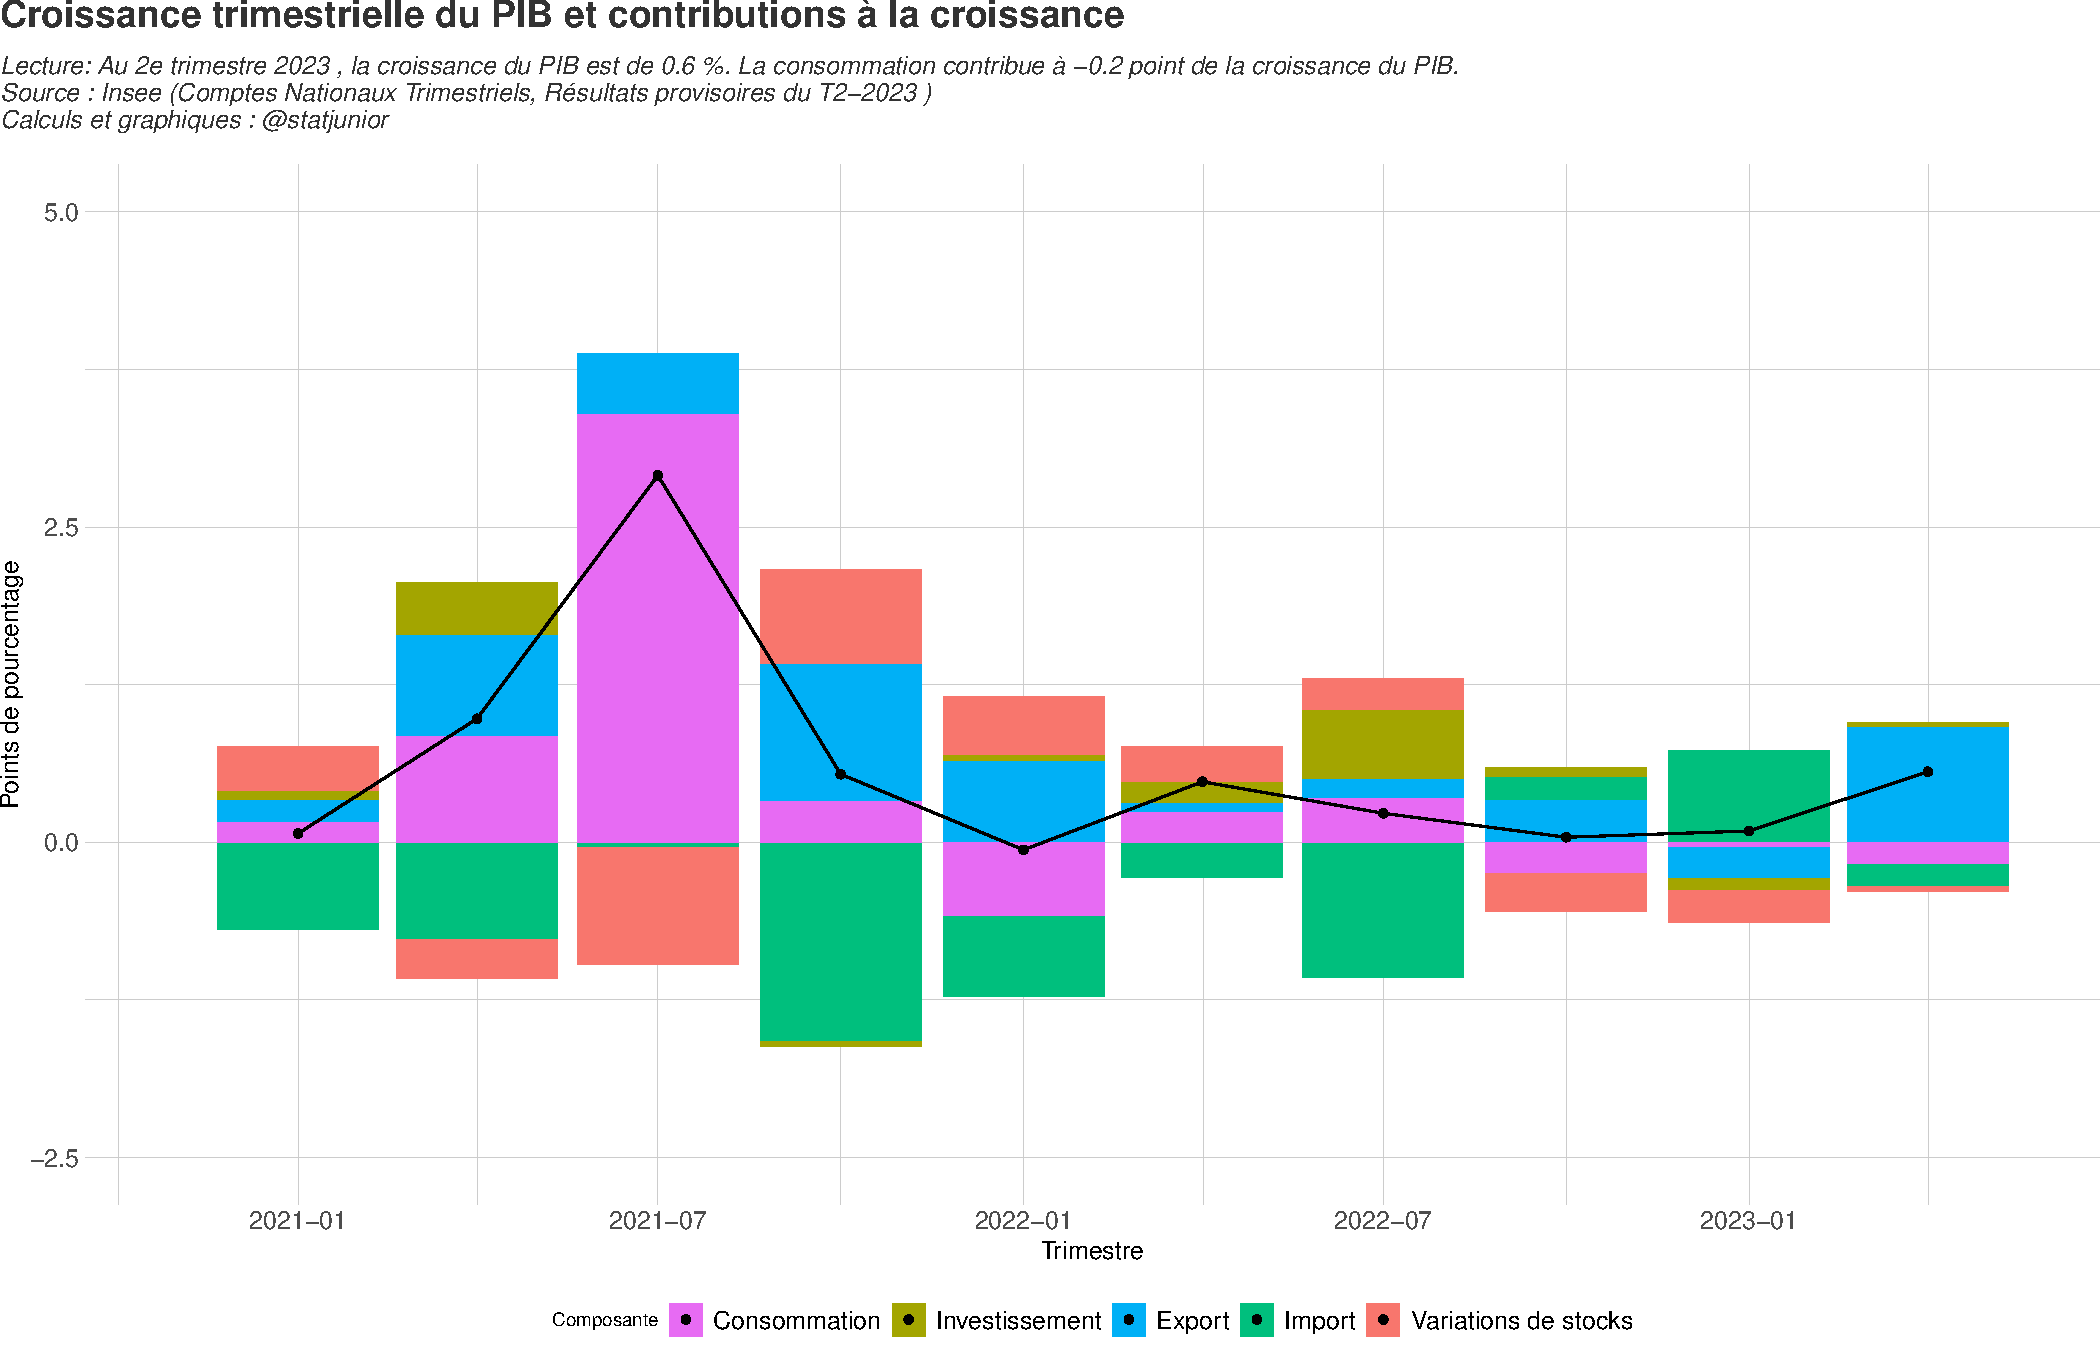
\includegraphics{rapport_pdf_compte_branche_files/figure-latex/unnamed-chunk-2-1.pdf}

\hypertarget{evolution-des-composantes-du-pib-en-volume-par-rapport-au-t4-2019}{%
\subsection{Evolution des composantes du PIB en volume par rapport au
T4-2019}\label{evolution-des-composantes-du-pib-en-volume-par-rapport-au-t4-2019}}

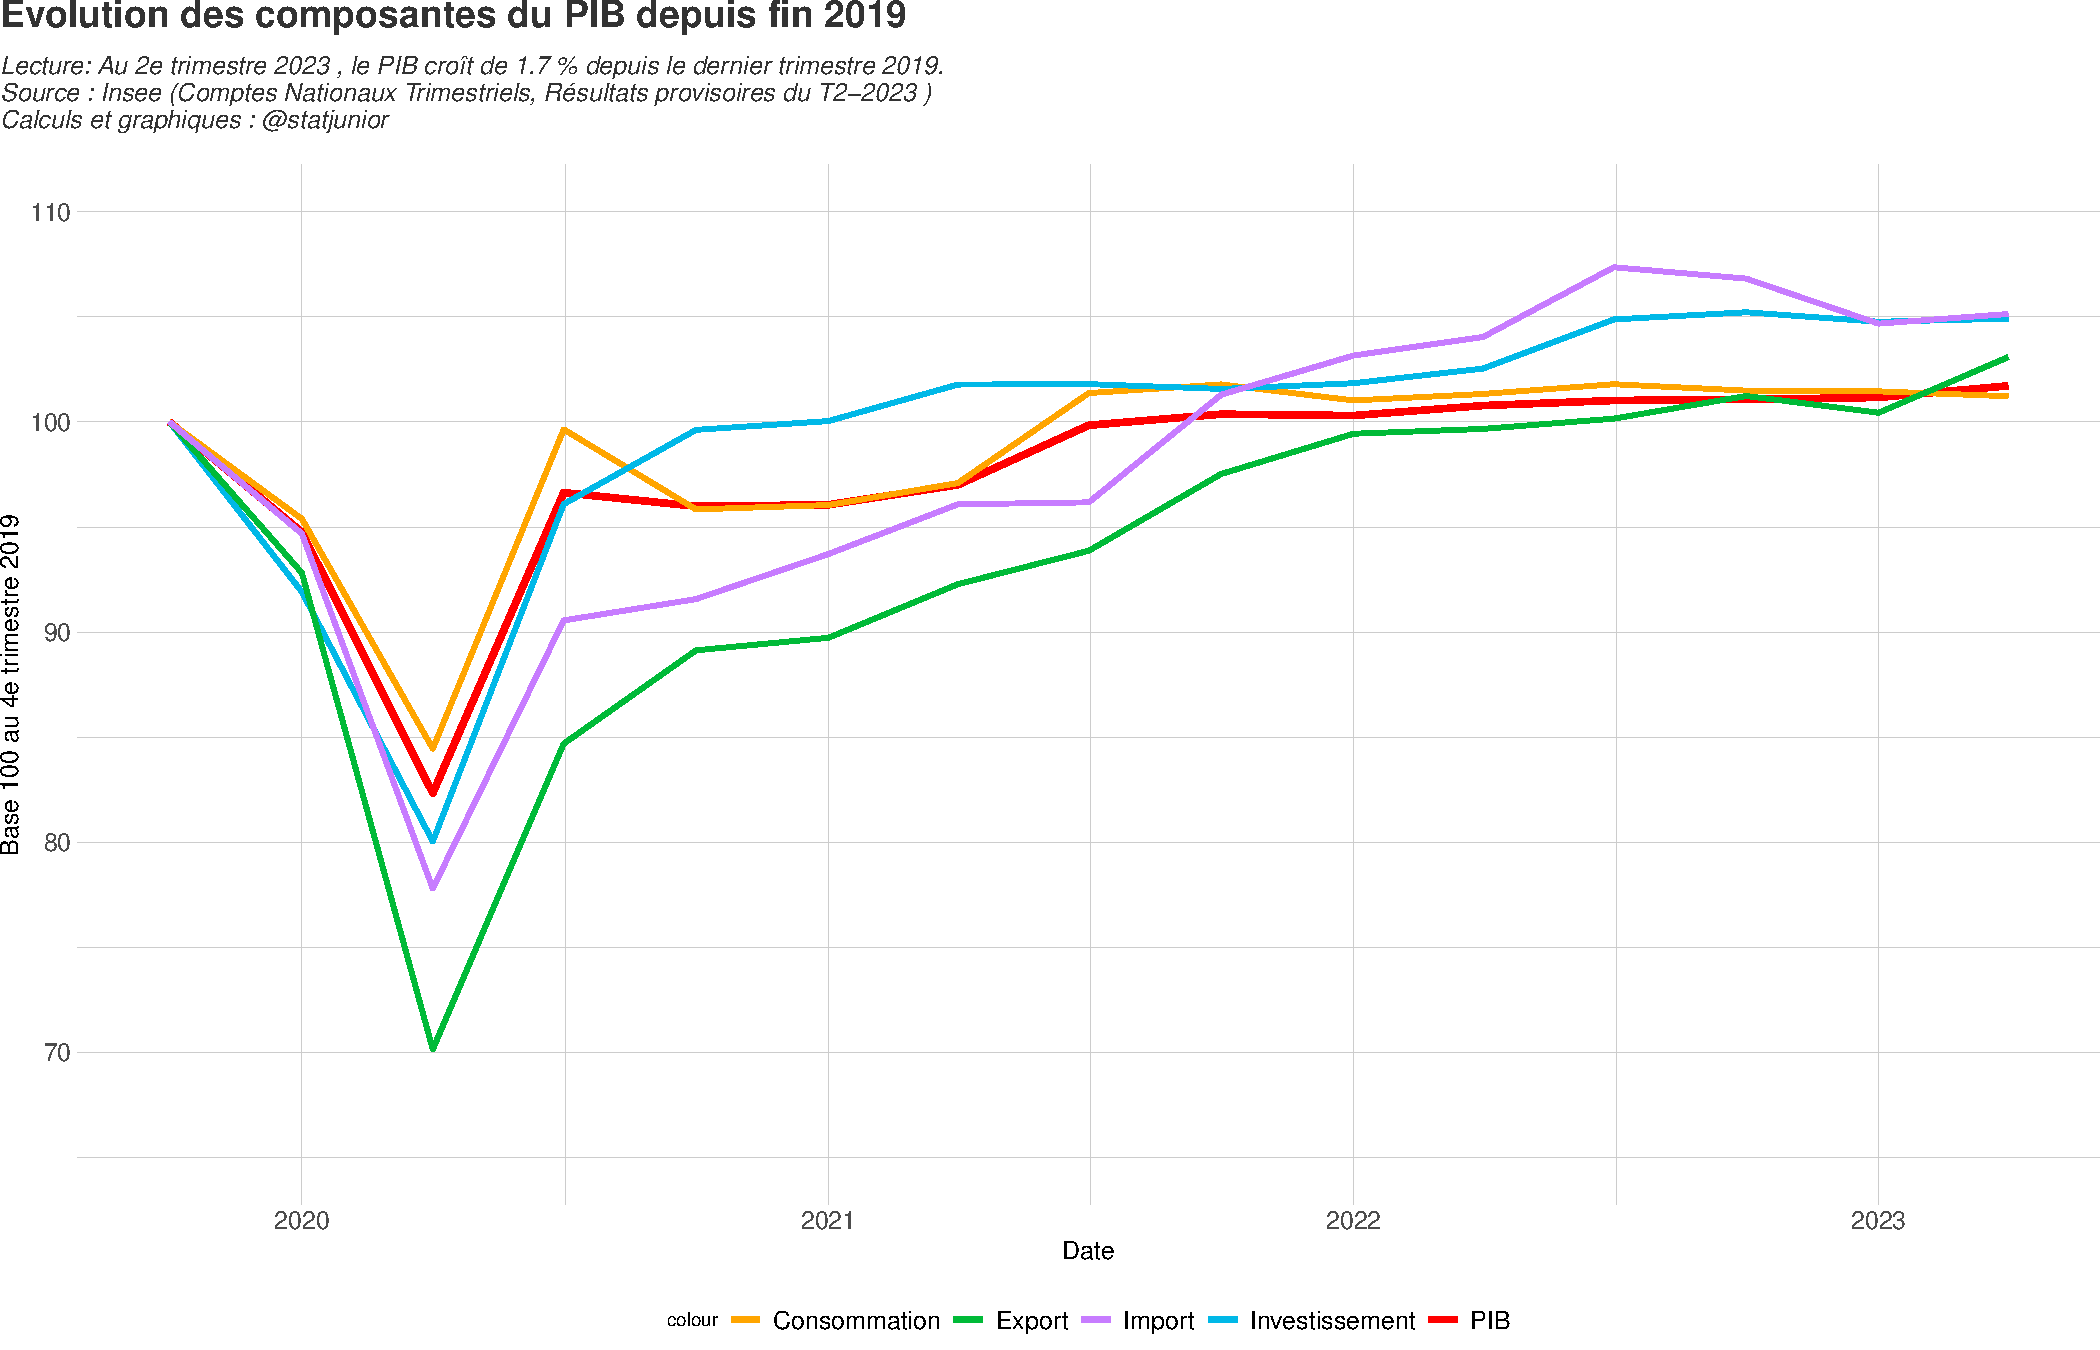
\includegraphics{rapport_pdf_compte_branche_files/figure-latex/unnamed-chunk-3-1.pdf}

\hypertarget{inflation-des-composantes-du-pib-au-dernier-trimestre-connu}{%
\subsection{Inflation des composantes du PIB au dernier trimestre
connu}\label{inflation-des-composantes-du-pib-au-dernier-trimestre-connu}}

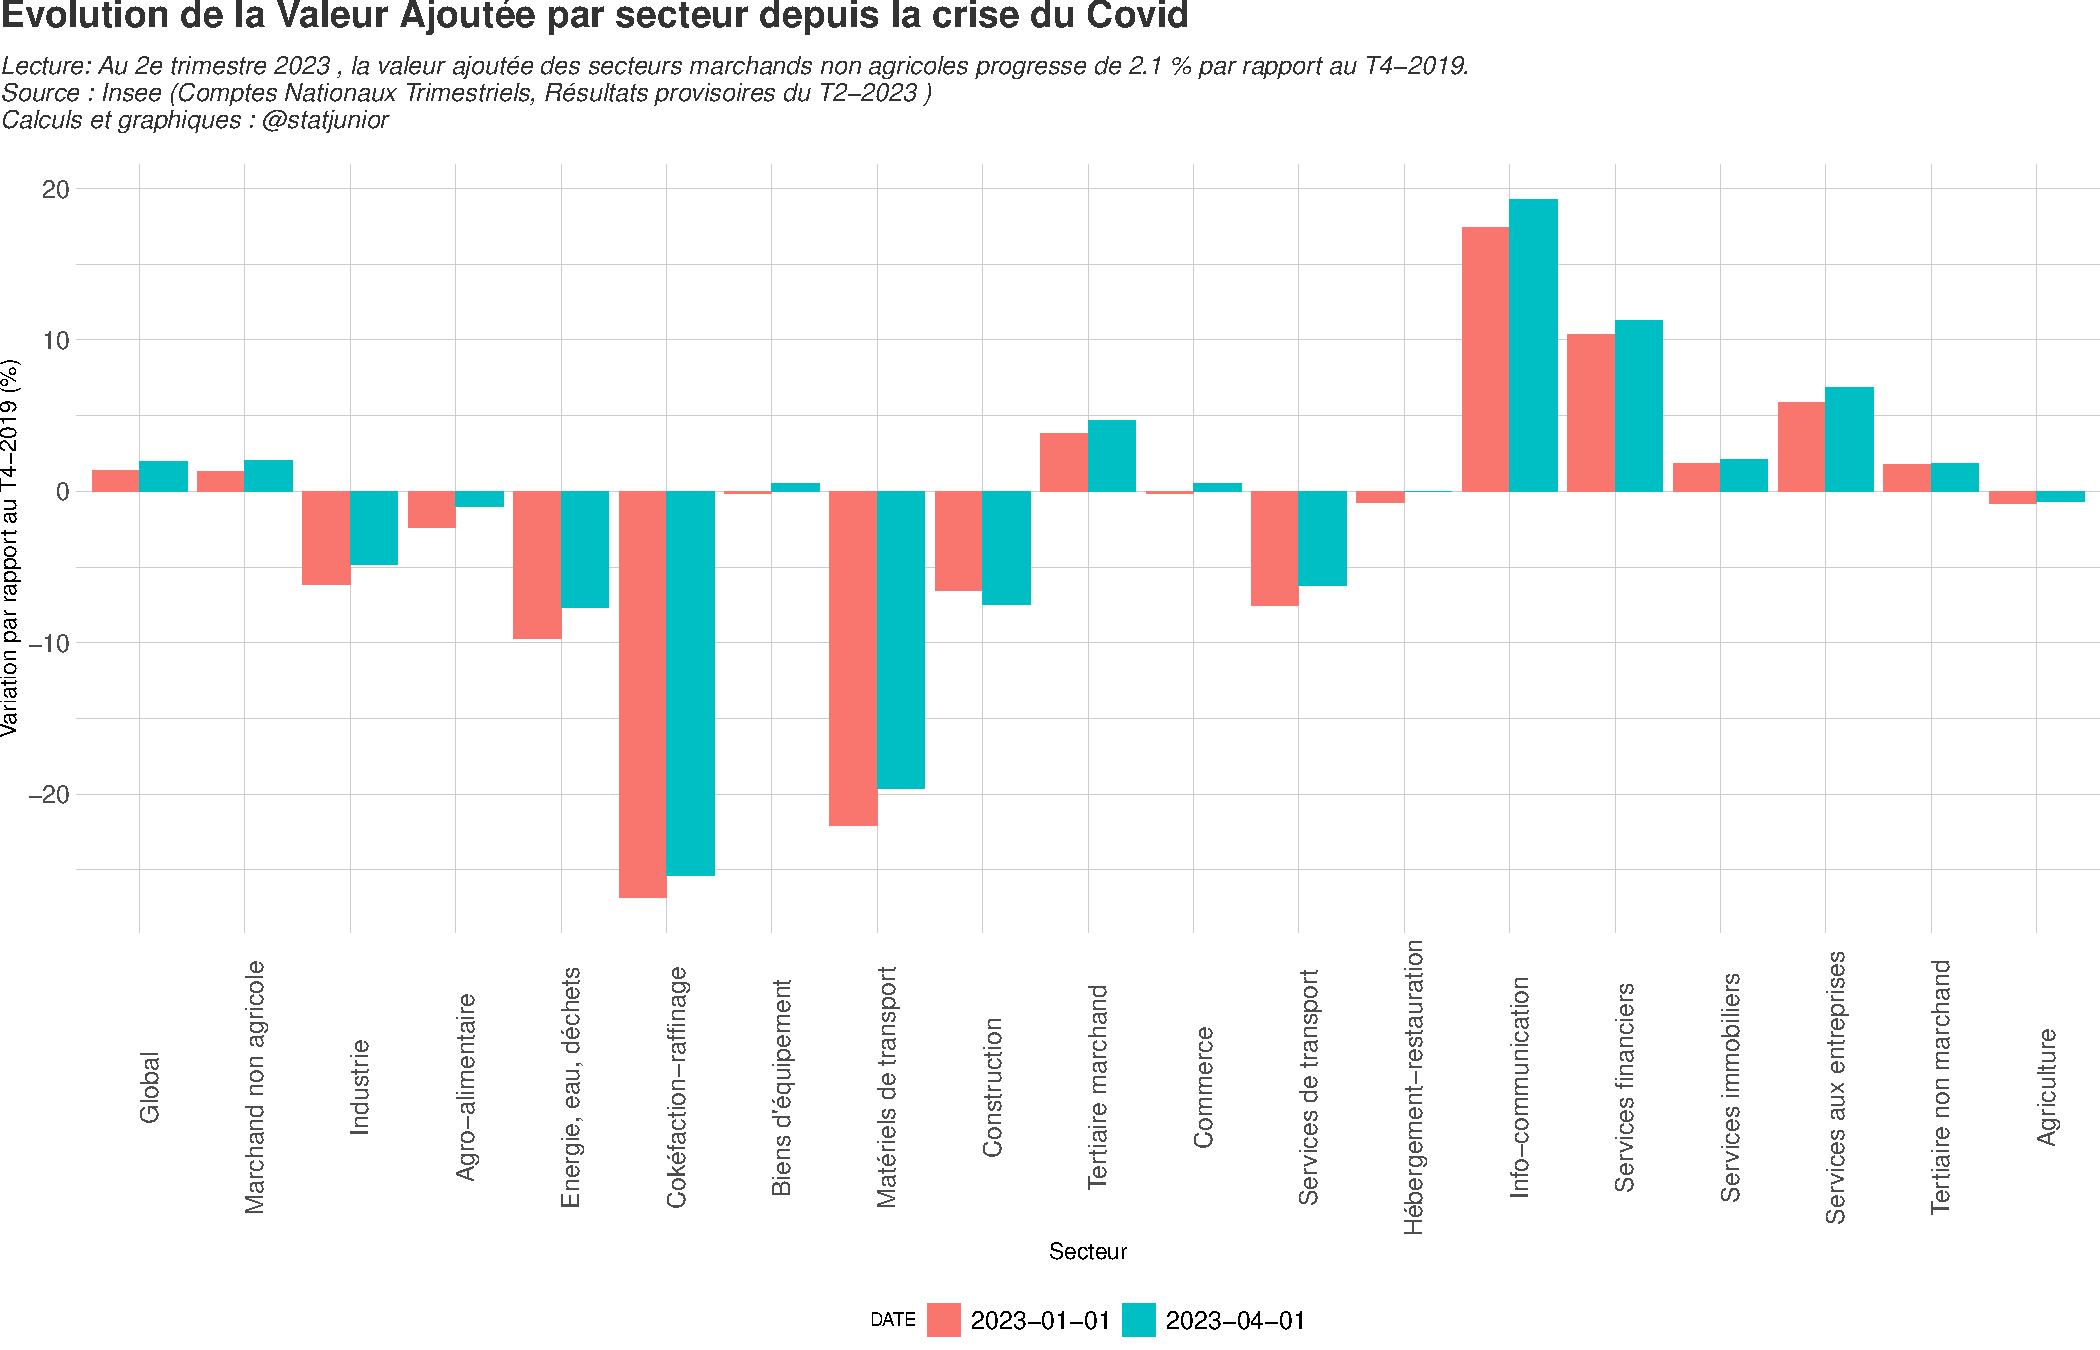
\includegraphics{rapport_pdf_compte_branche_files/figure-latex/unnamed-chunk-4-1.pdf}

\hypertarget{prix-des-composantes-du-pib-depuis-la-fin-2019}{%
\subsection{Prix des composantes du PIB depuis la fin
2019}\label{prix-des-composantes-du-pib-depuis-la-fin-2019}}

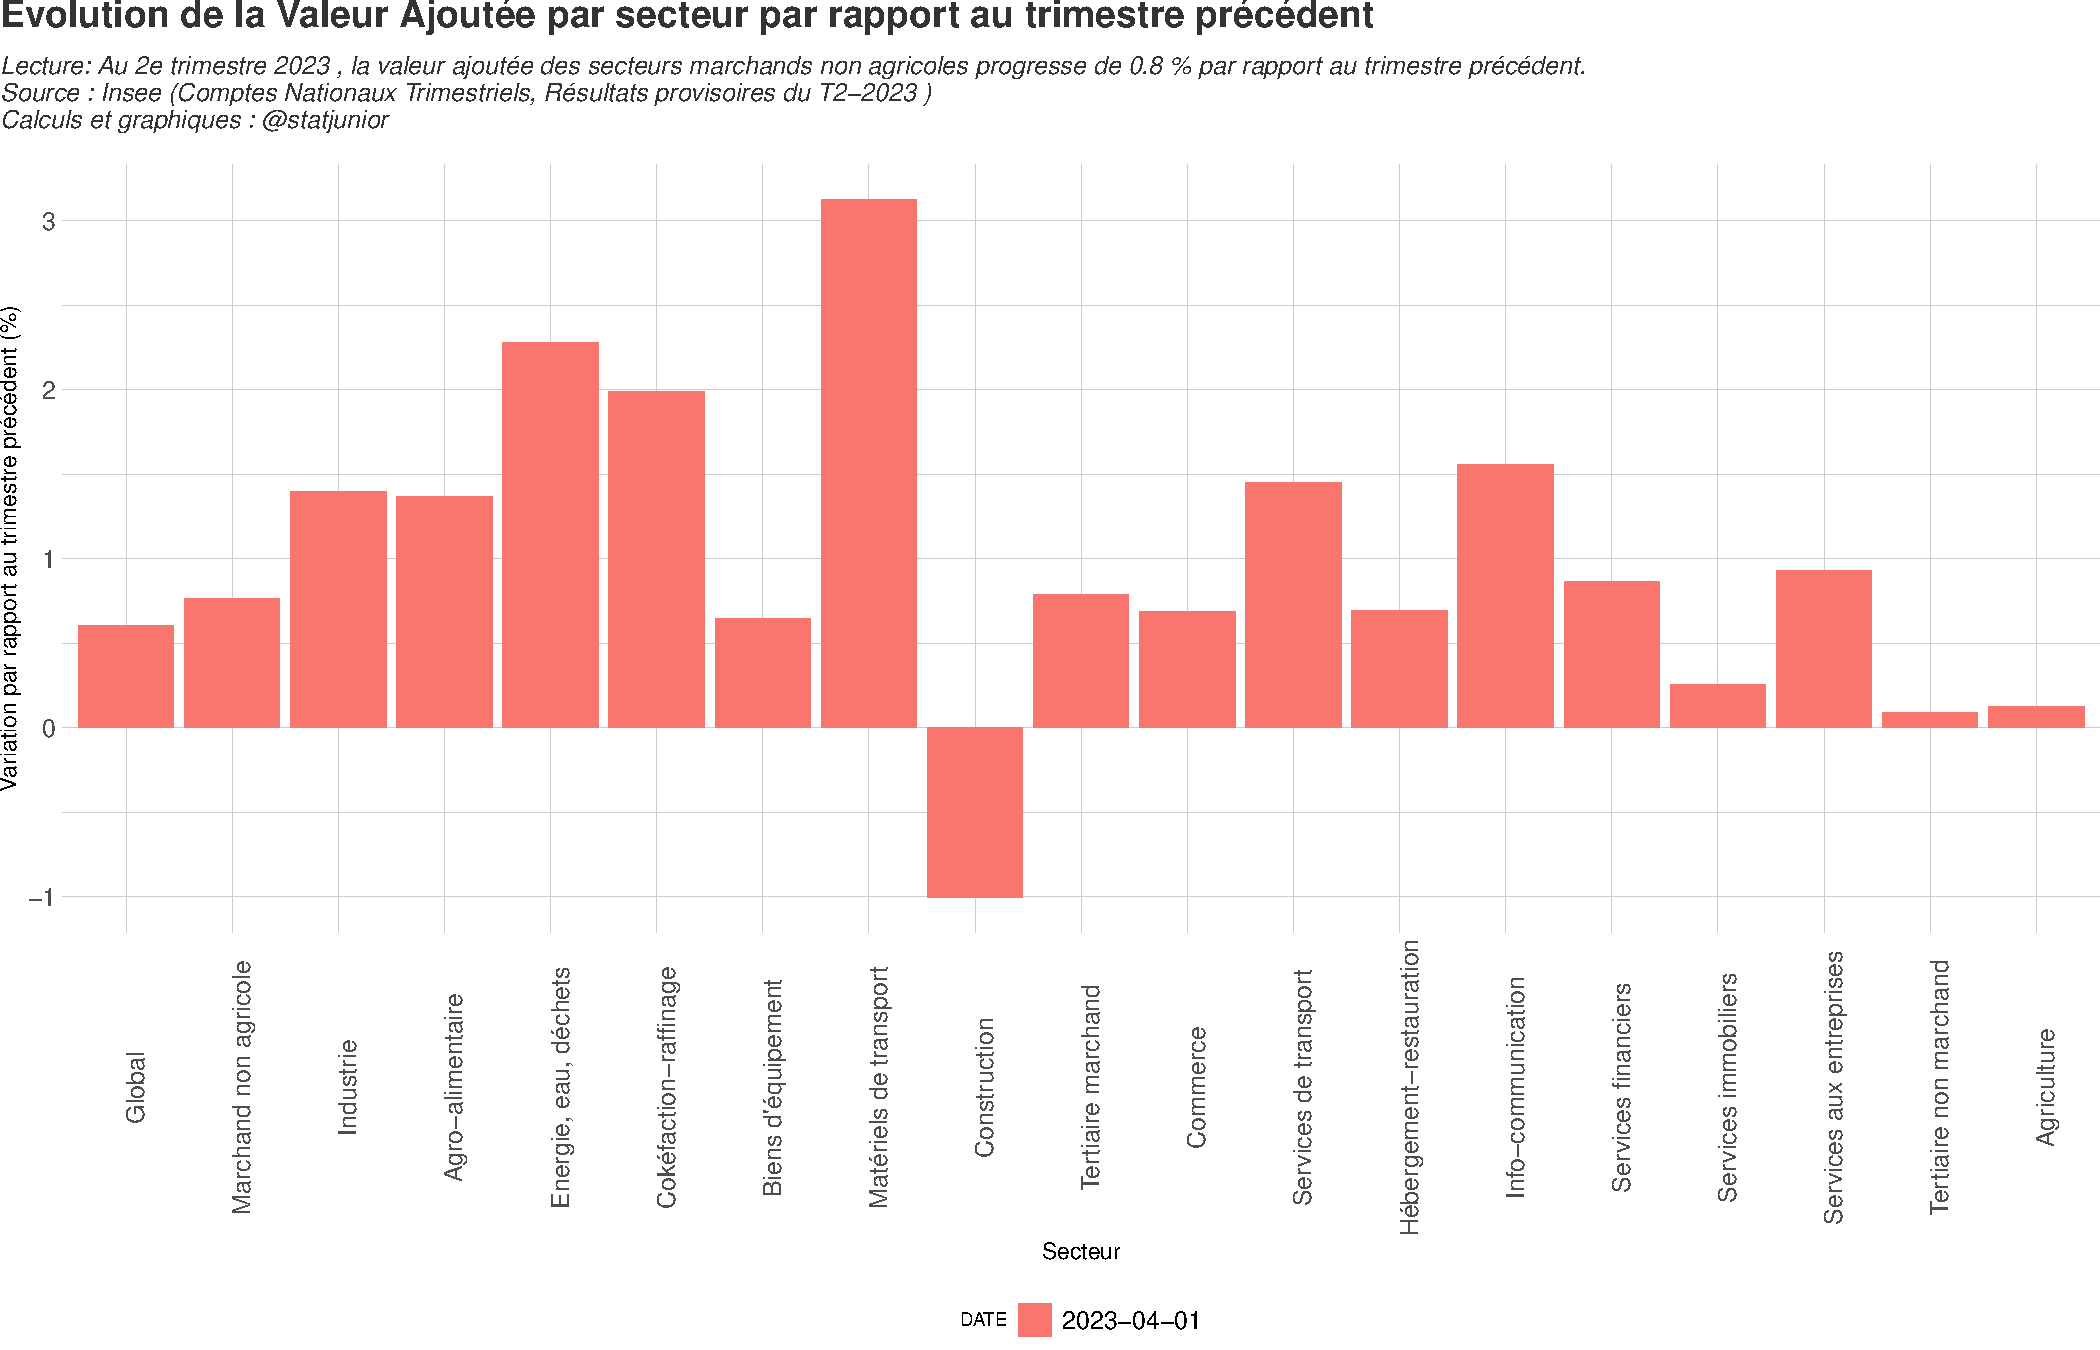
\includegraphics{rapport_pdf_compte_branche_files/figure-latex/unnamed-chunk-5-1.pdf}

\newpage

\hypertarget{solde-des-uxe9changes-extuxe9rieurs-de-la-france}{%
\section{Solde des échanges extérieurs de la
France}\label{solde-des-uxe9changes-extuxe9rieurs-de-la-france}}

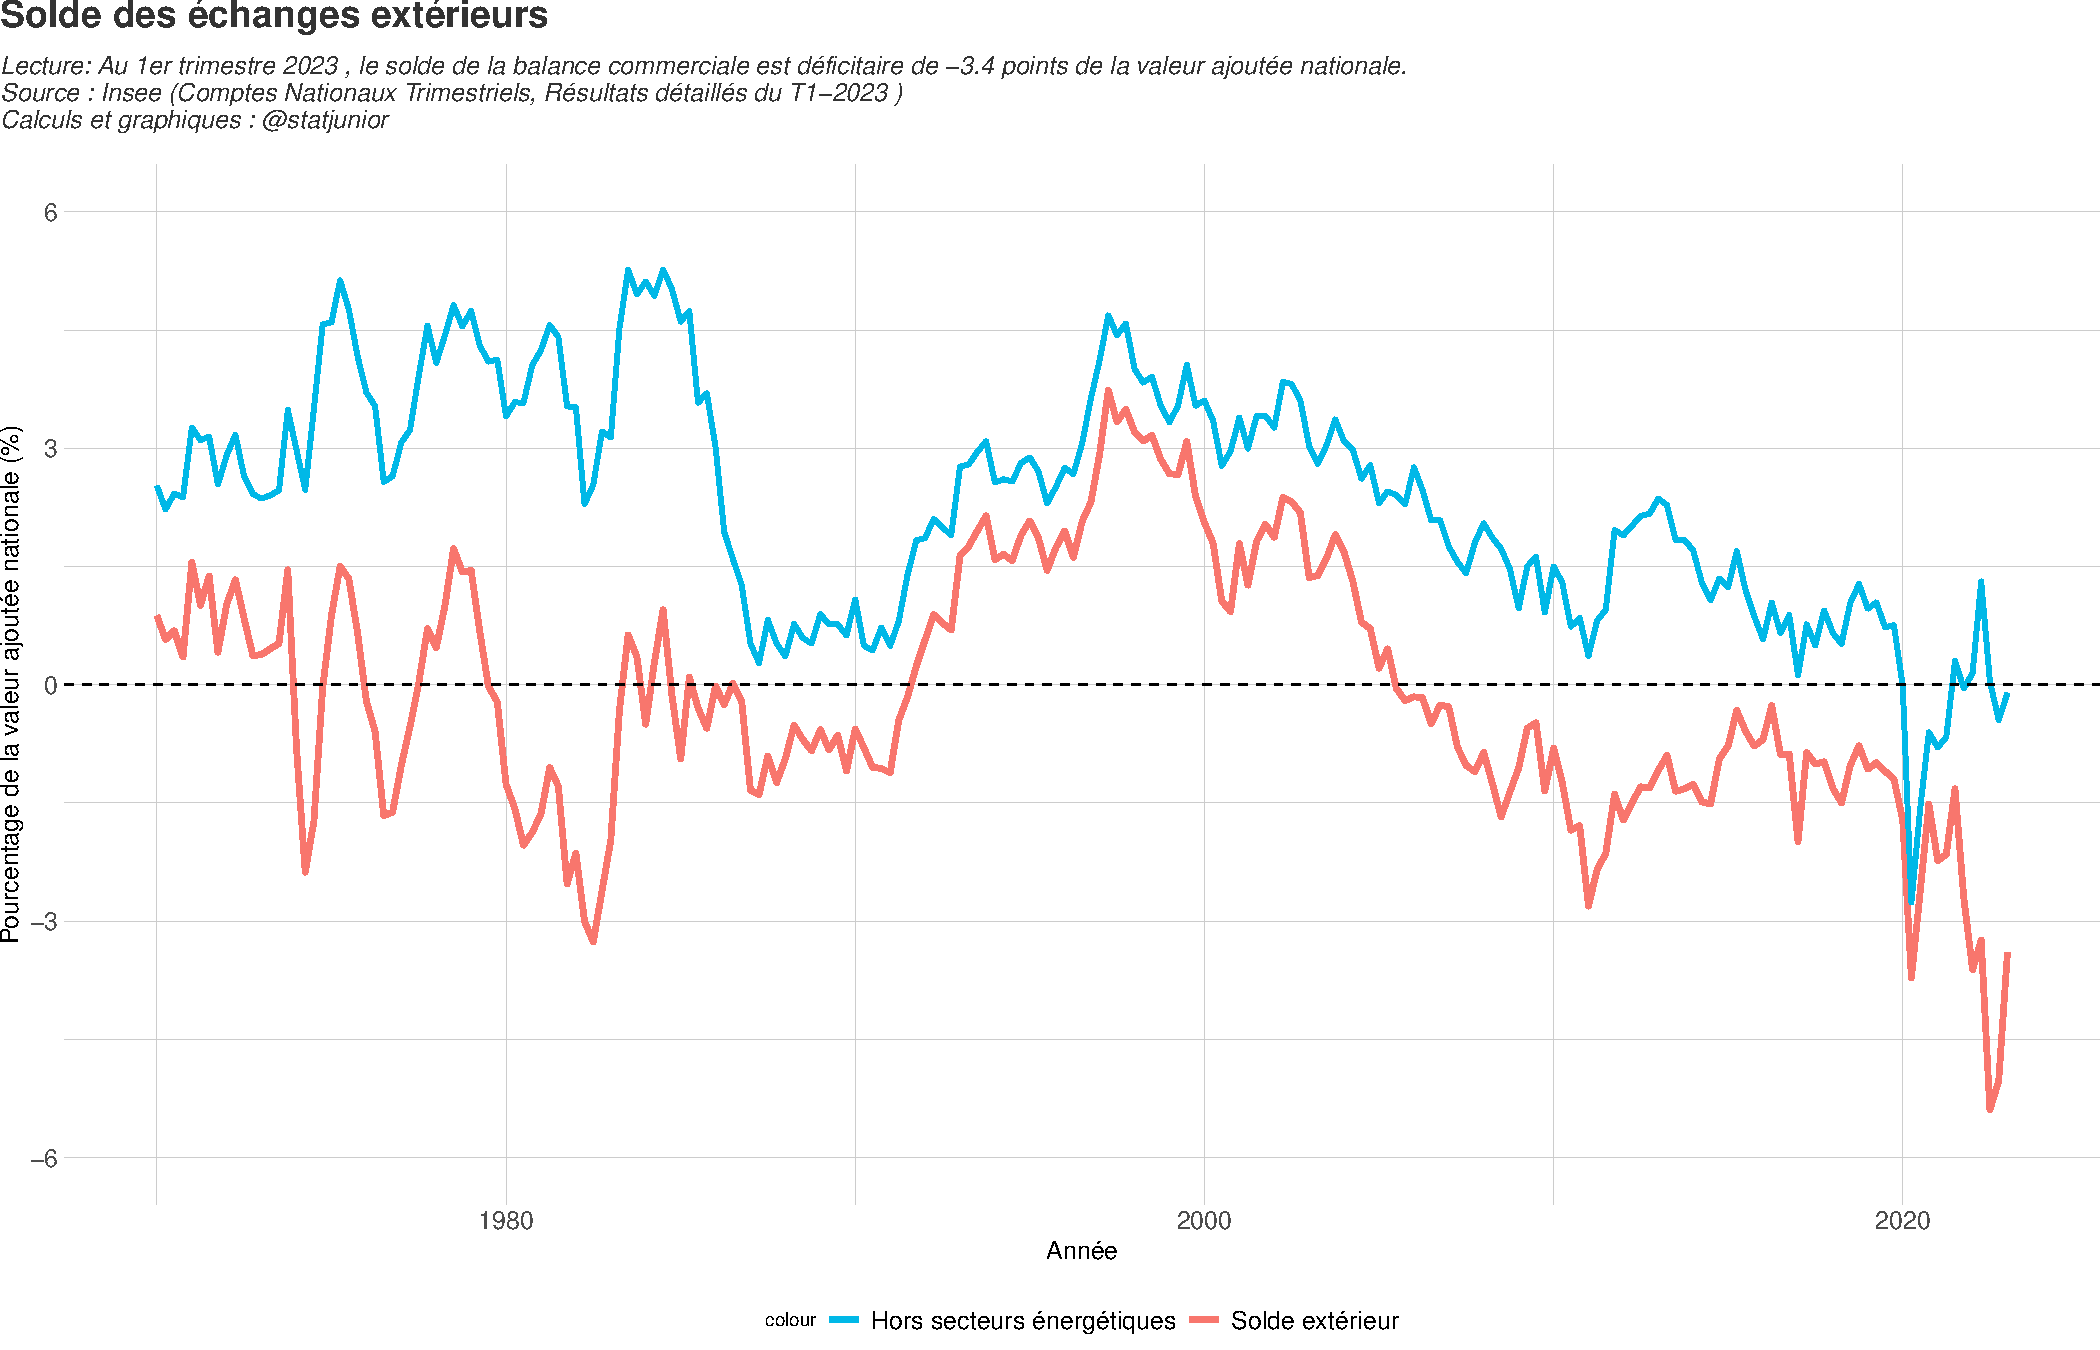
\includegraphics{rapport_pdf_compte_branche_files/figure-latex/unnamed-chunk-6-1.pdf}

\newpage

\hypertarget{consommation}{%
\section{Consommation}\label{consommation}}

\hypertarget{consommation-uxe9nerguxe9tique-et-agro-alimentaire-en-volume-depuis-fin-2019}{%
\subsection{Consommation énergétique et agro-alimentaire en volume
depuis fin
2019}\label{consommation-uxe9nerguxe9tique-et-agro-alimentaire-en-volume-depuis-fin-2019}}

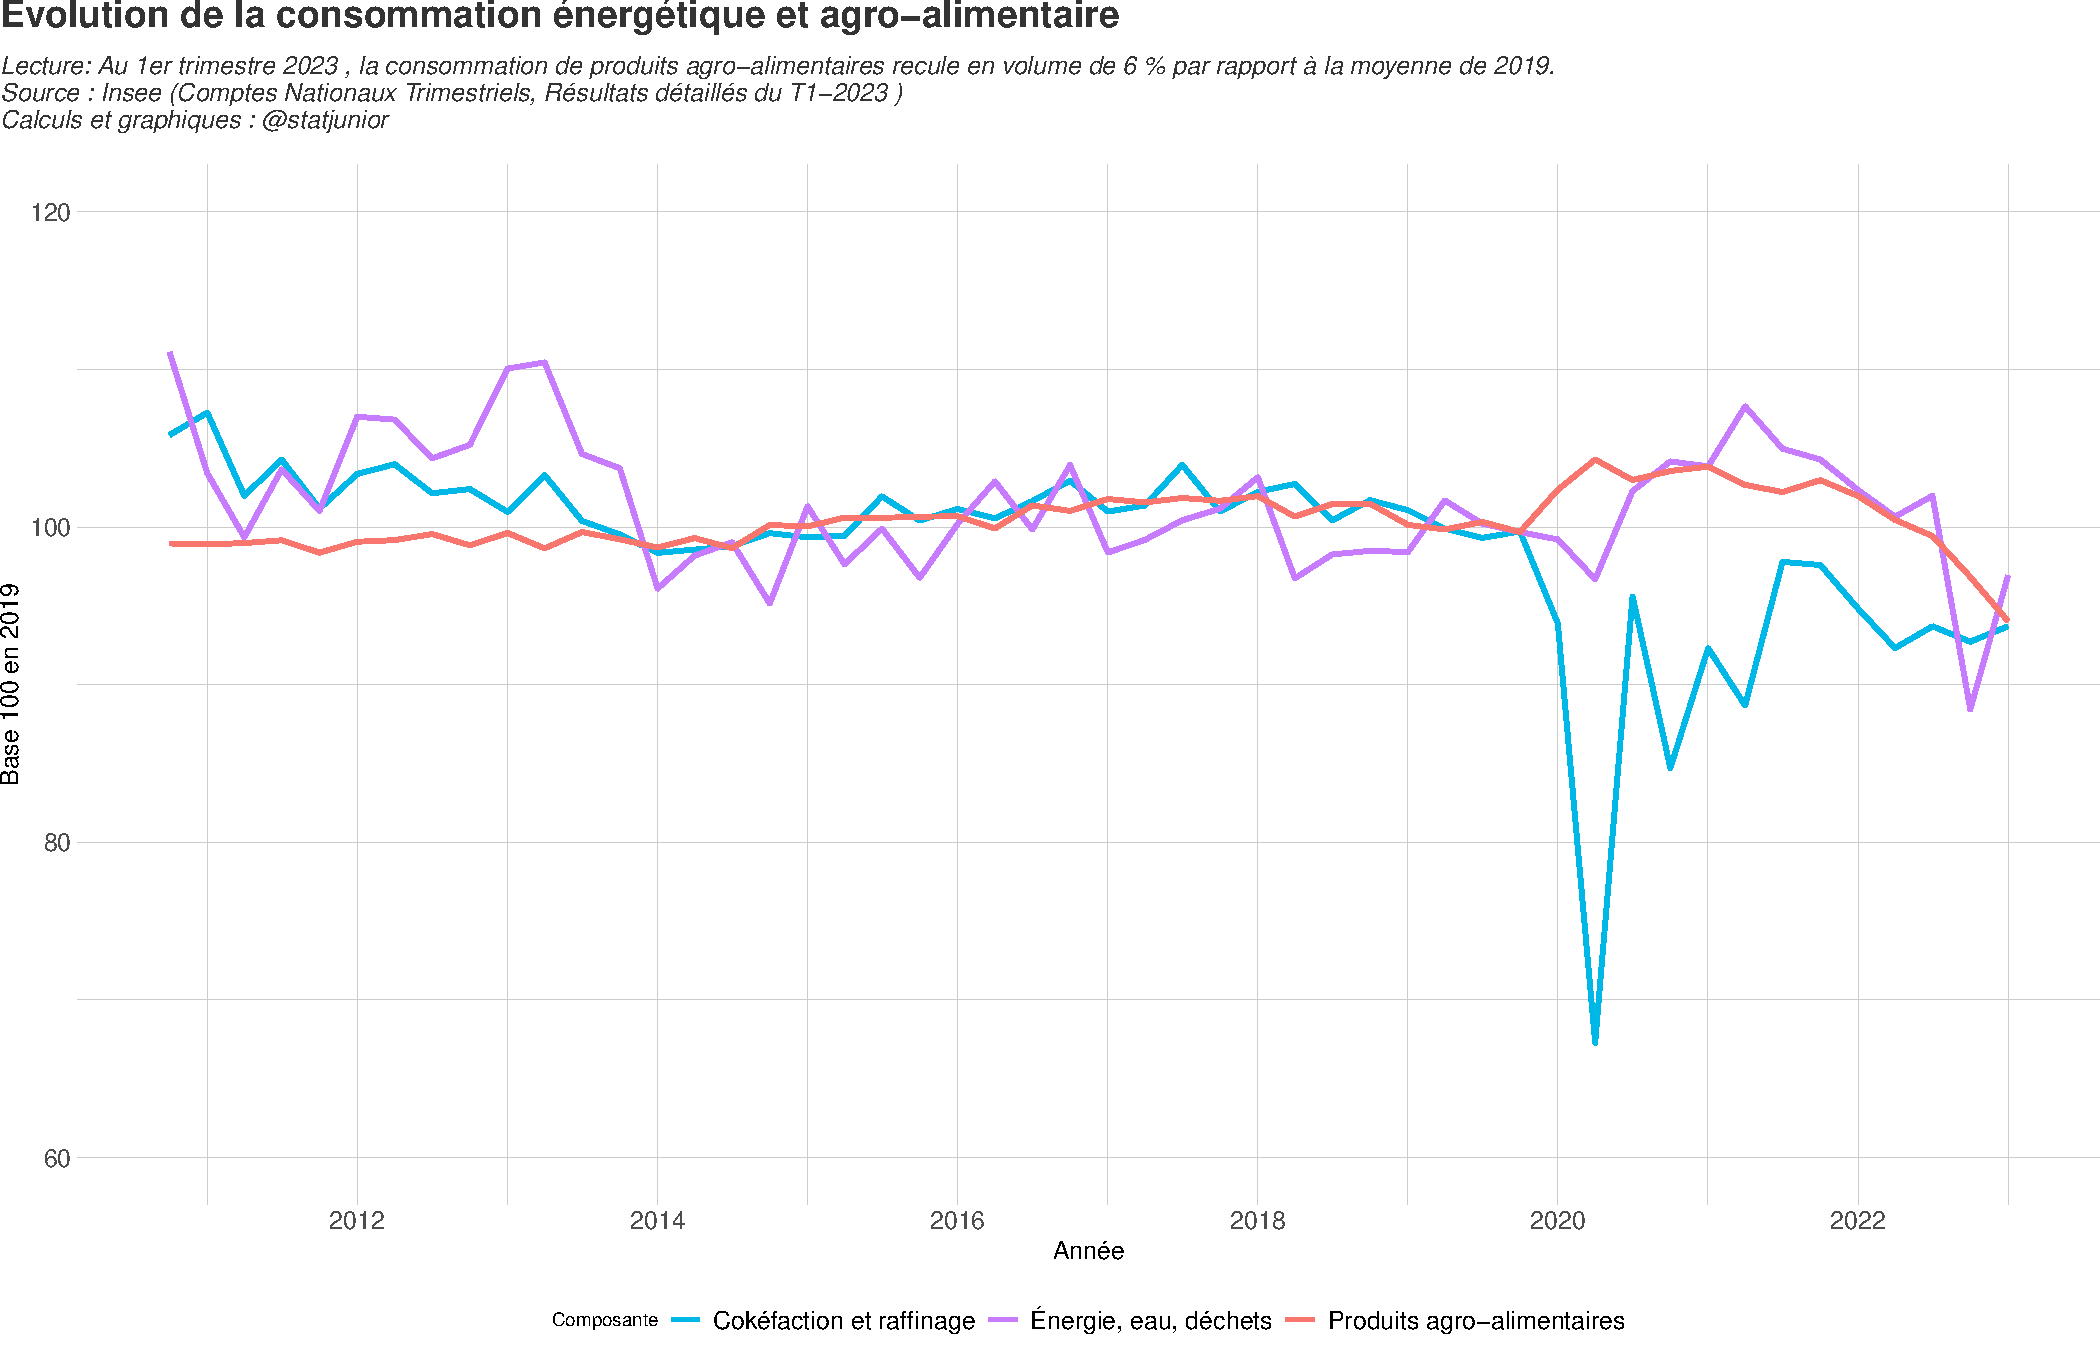
\includegraphics{rapport_pdf_compte_branche_files/figure-latex/unnamed-chunk-8-1.pdf}

\hypertarget{evolution-sur-longue-puxe9riode-de-la-consommation-alimentaire-en-volume}{%
\subsection{Evolution sur longue période de la consommation alimentaire
en
volume}\label{evolution-sur-longue-puxe9riode-de-la-consommation-alimentaire-en-volume}}

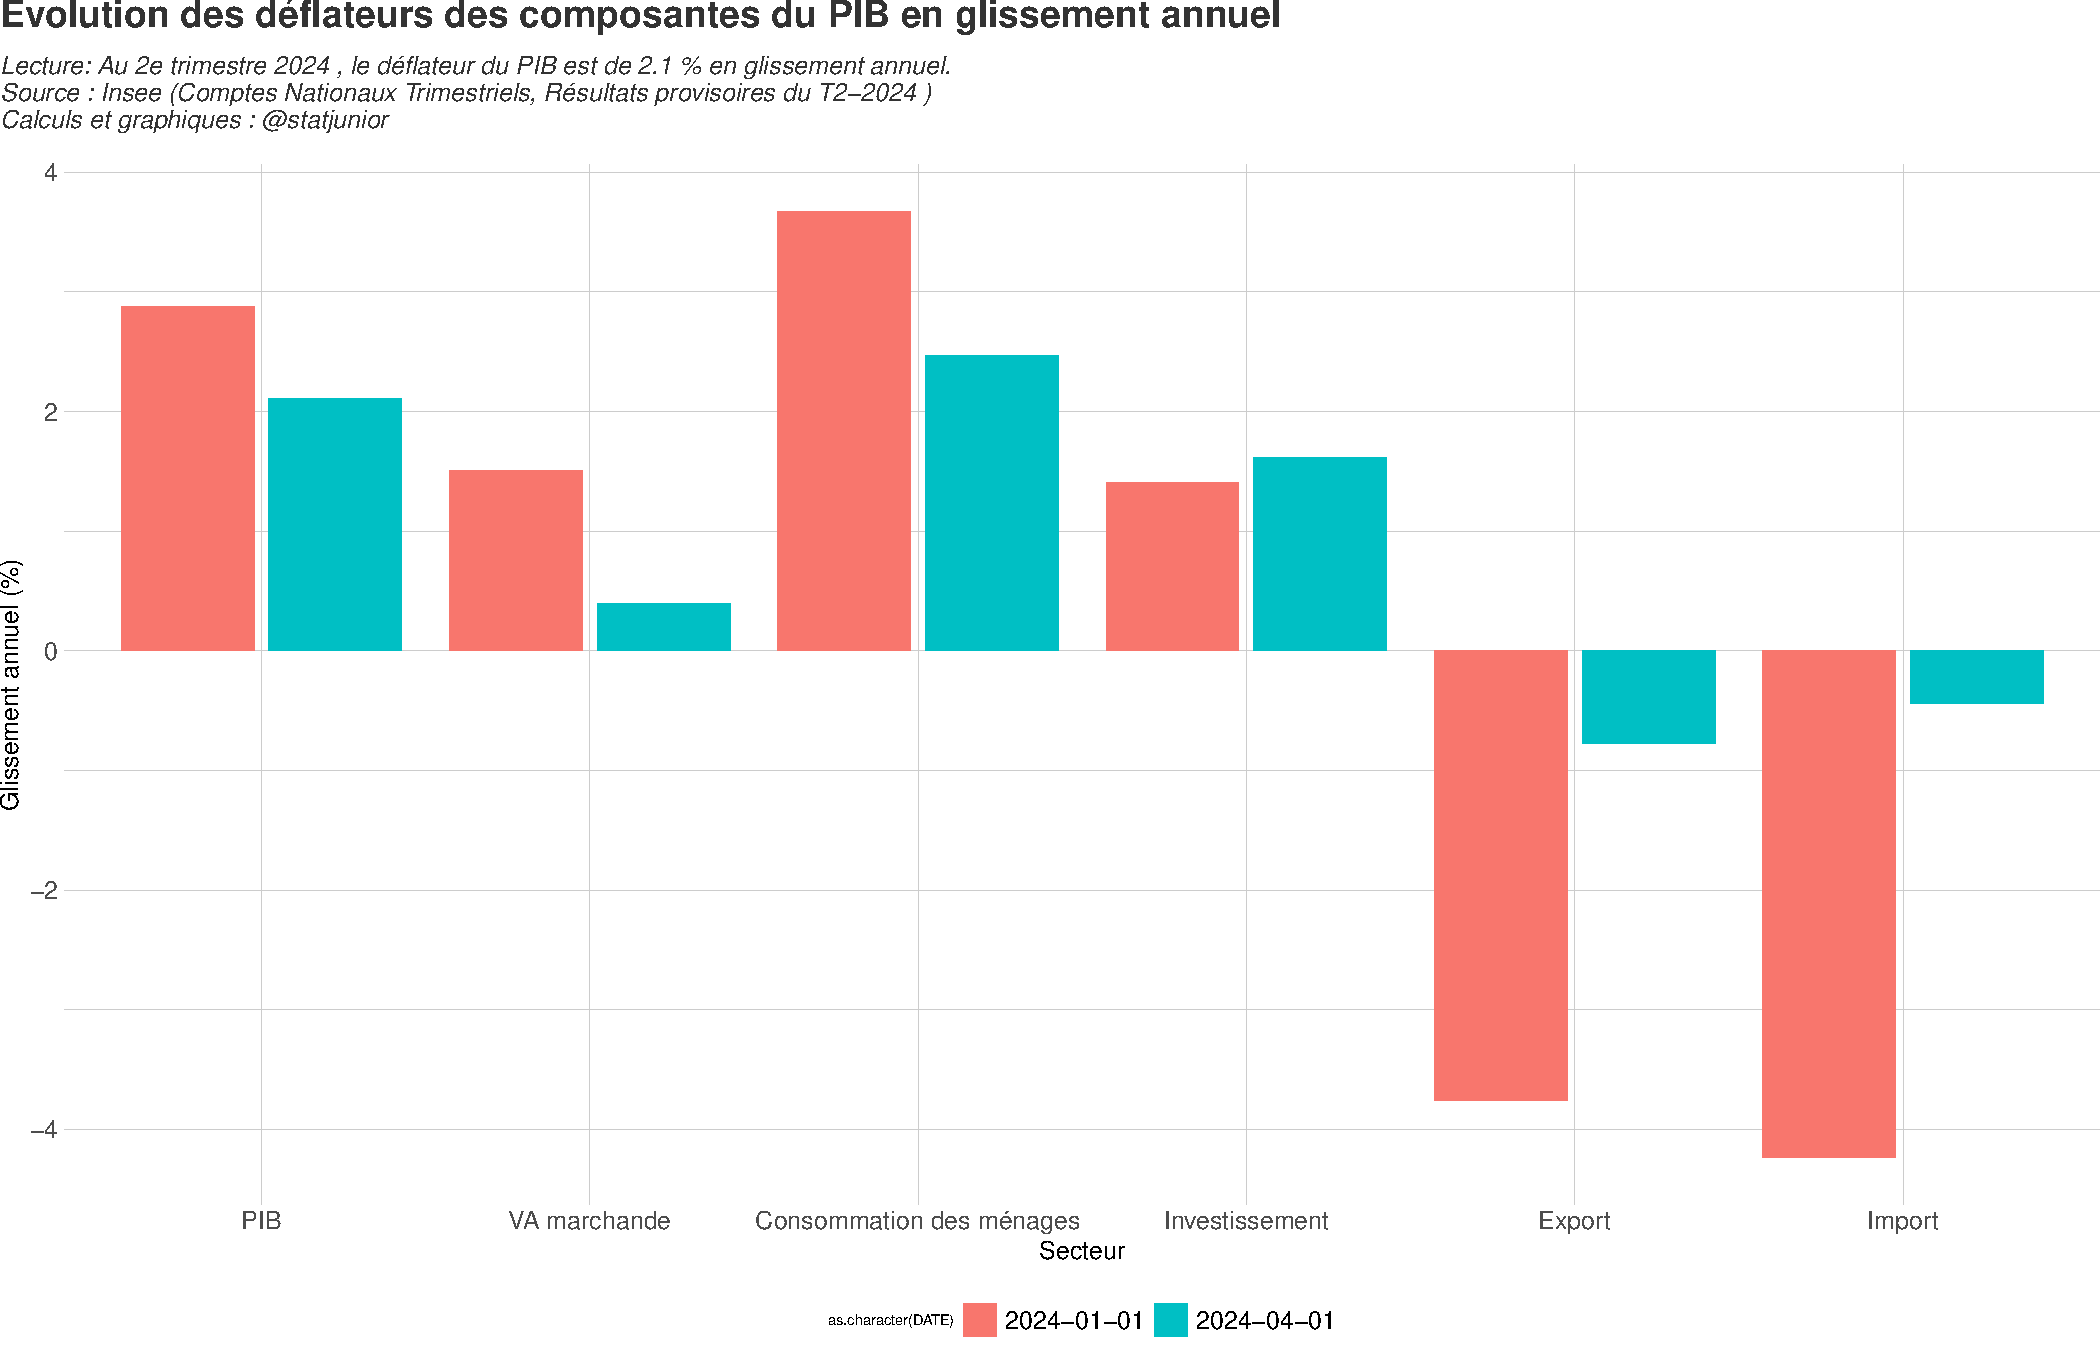
\includegraphics{rapport_pdf_compte_branche_files/figure-latex/unnamed-chunk-9-1.pdf}

\newpage

\hypertarget{salaires-masse-salariale-et-productivituxe9-du-travail}{%
\section{Salaires, Masse salariale et Productivité du
travail}\label{salaires-masse-salariale-et-productivituxe9-du-travail}}

\hypertarget{evolution-de-la-valeur-ajoutuxe9e-et-de-la-productivituxe9-du-travail-depuis-2000}{%
\subsection{Evolution de la valeur ajoutée et de la productivité du
travail depuis
2000}\label{evolution-de-la-valeur-ajoutuxe9e-et-de-la-productivituxe9-du-travail-depuis-2000}}

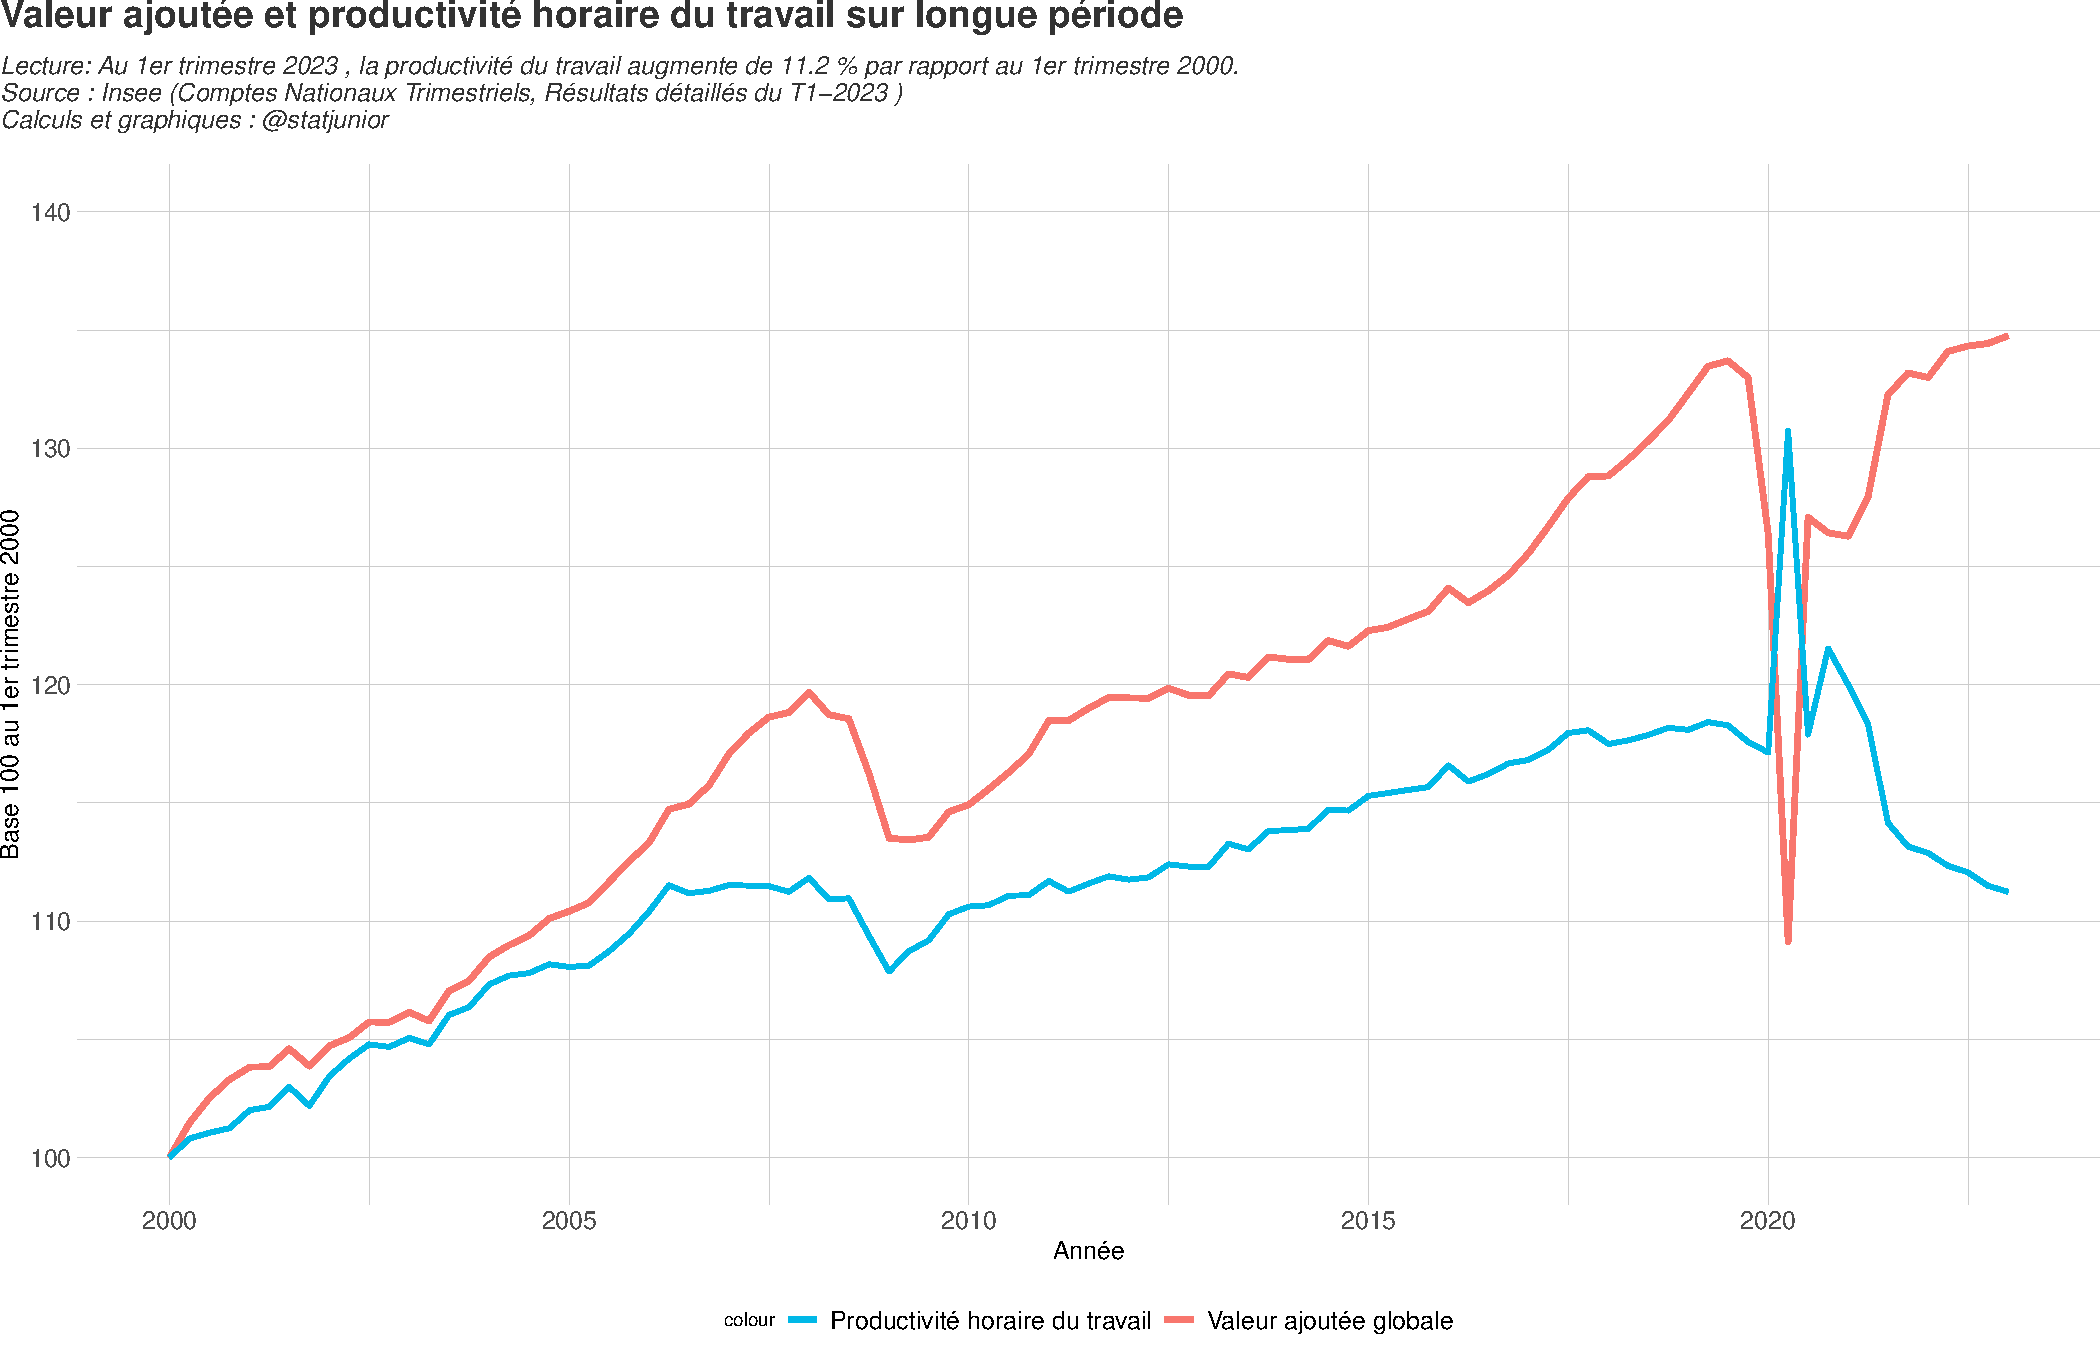
\includegraphics{rapport_pdf_compte_branche_files/figure-latex/unnamed-chunk-10-1.pdf}

\hypertarget{evolution-de-la-valeur-ajoutuxe9e-et-de-la-productivituxe9-du-travail-depuis-2019}{%
\subsection{Evolution de la valeur ajoutée et de la productivité du
travail depuis
2019}\label{evolution-de-la-valeur-ajoutuxe9e-et-de-la-productivituxe9-du-travail-depuis-2019}}

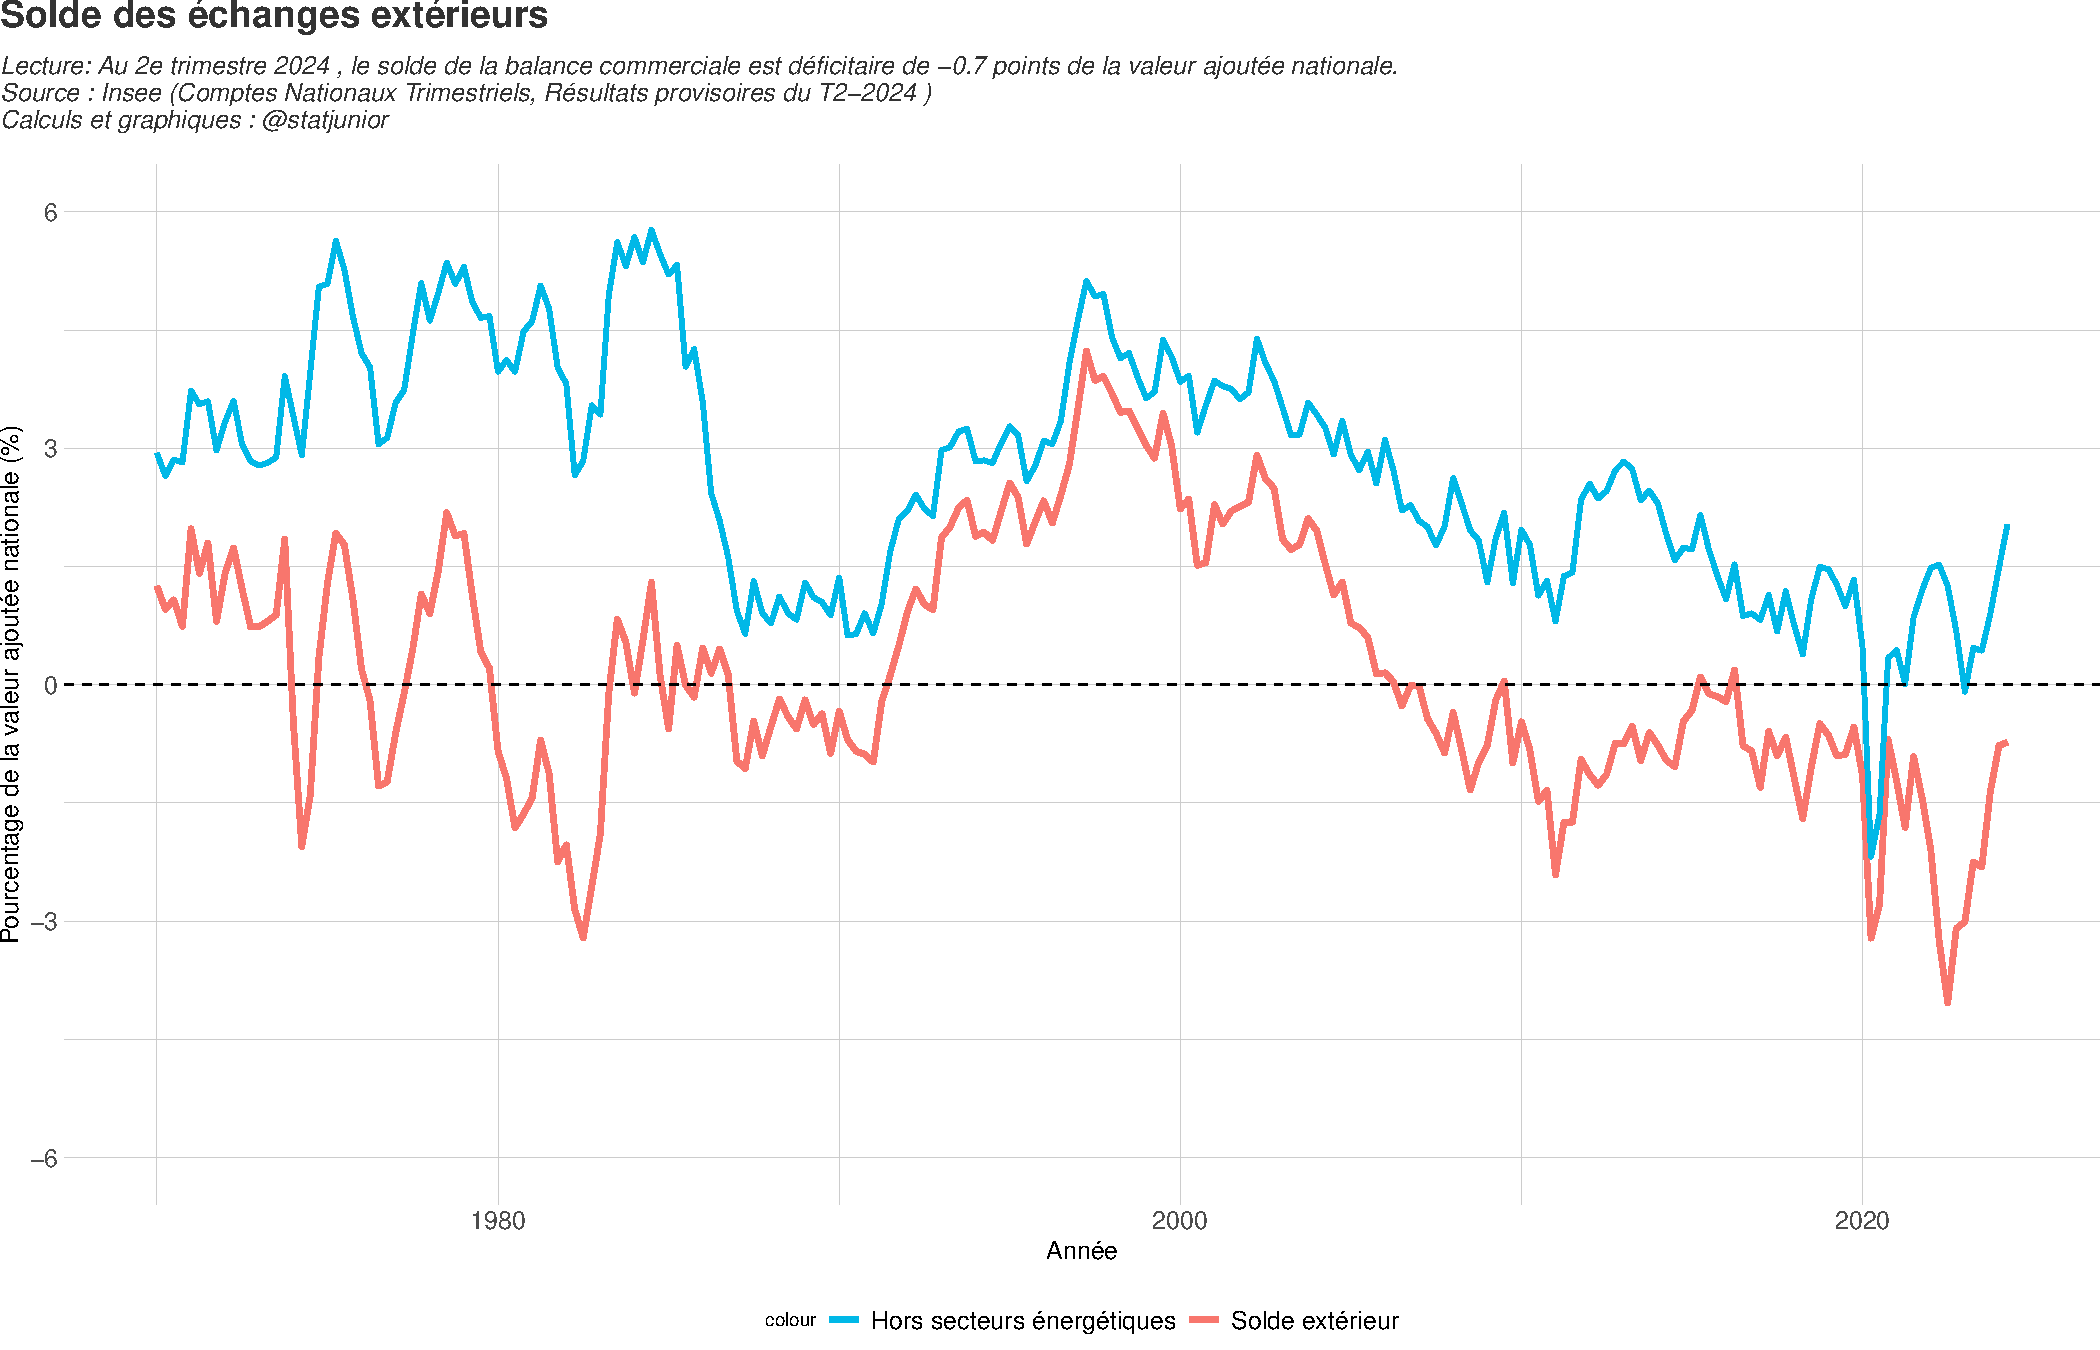
\includegraphics{rapport_pdf_compte_branche_files/figure-latex/unnamed-chunk-11-1.pdf}

\hypertarget{evolution-de-la-productivituxe9-par-tuxeate-et-de-la-productivituxe9-apparente-du-travail-depuis-2019}{%
\subsection{Evolution de la Productivité par Tête et de la Productivité
apparente du travail depuis
2019}\label{evolution-de-la-productivituxe9-par-tuxeate-et-de-la-productivituxe9-apparente-du-travail-depuis-2019}}

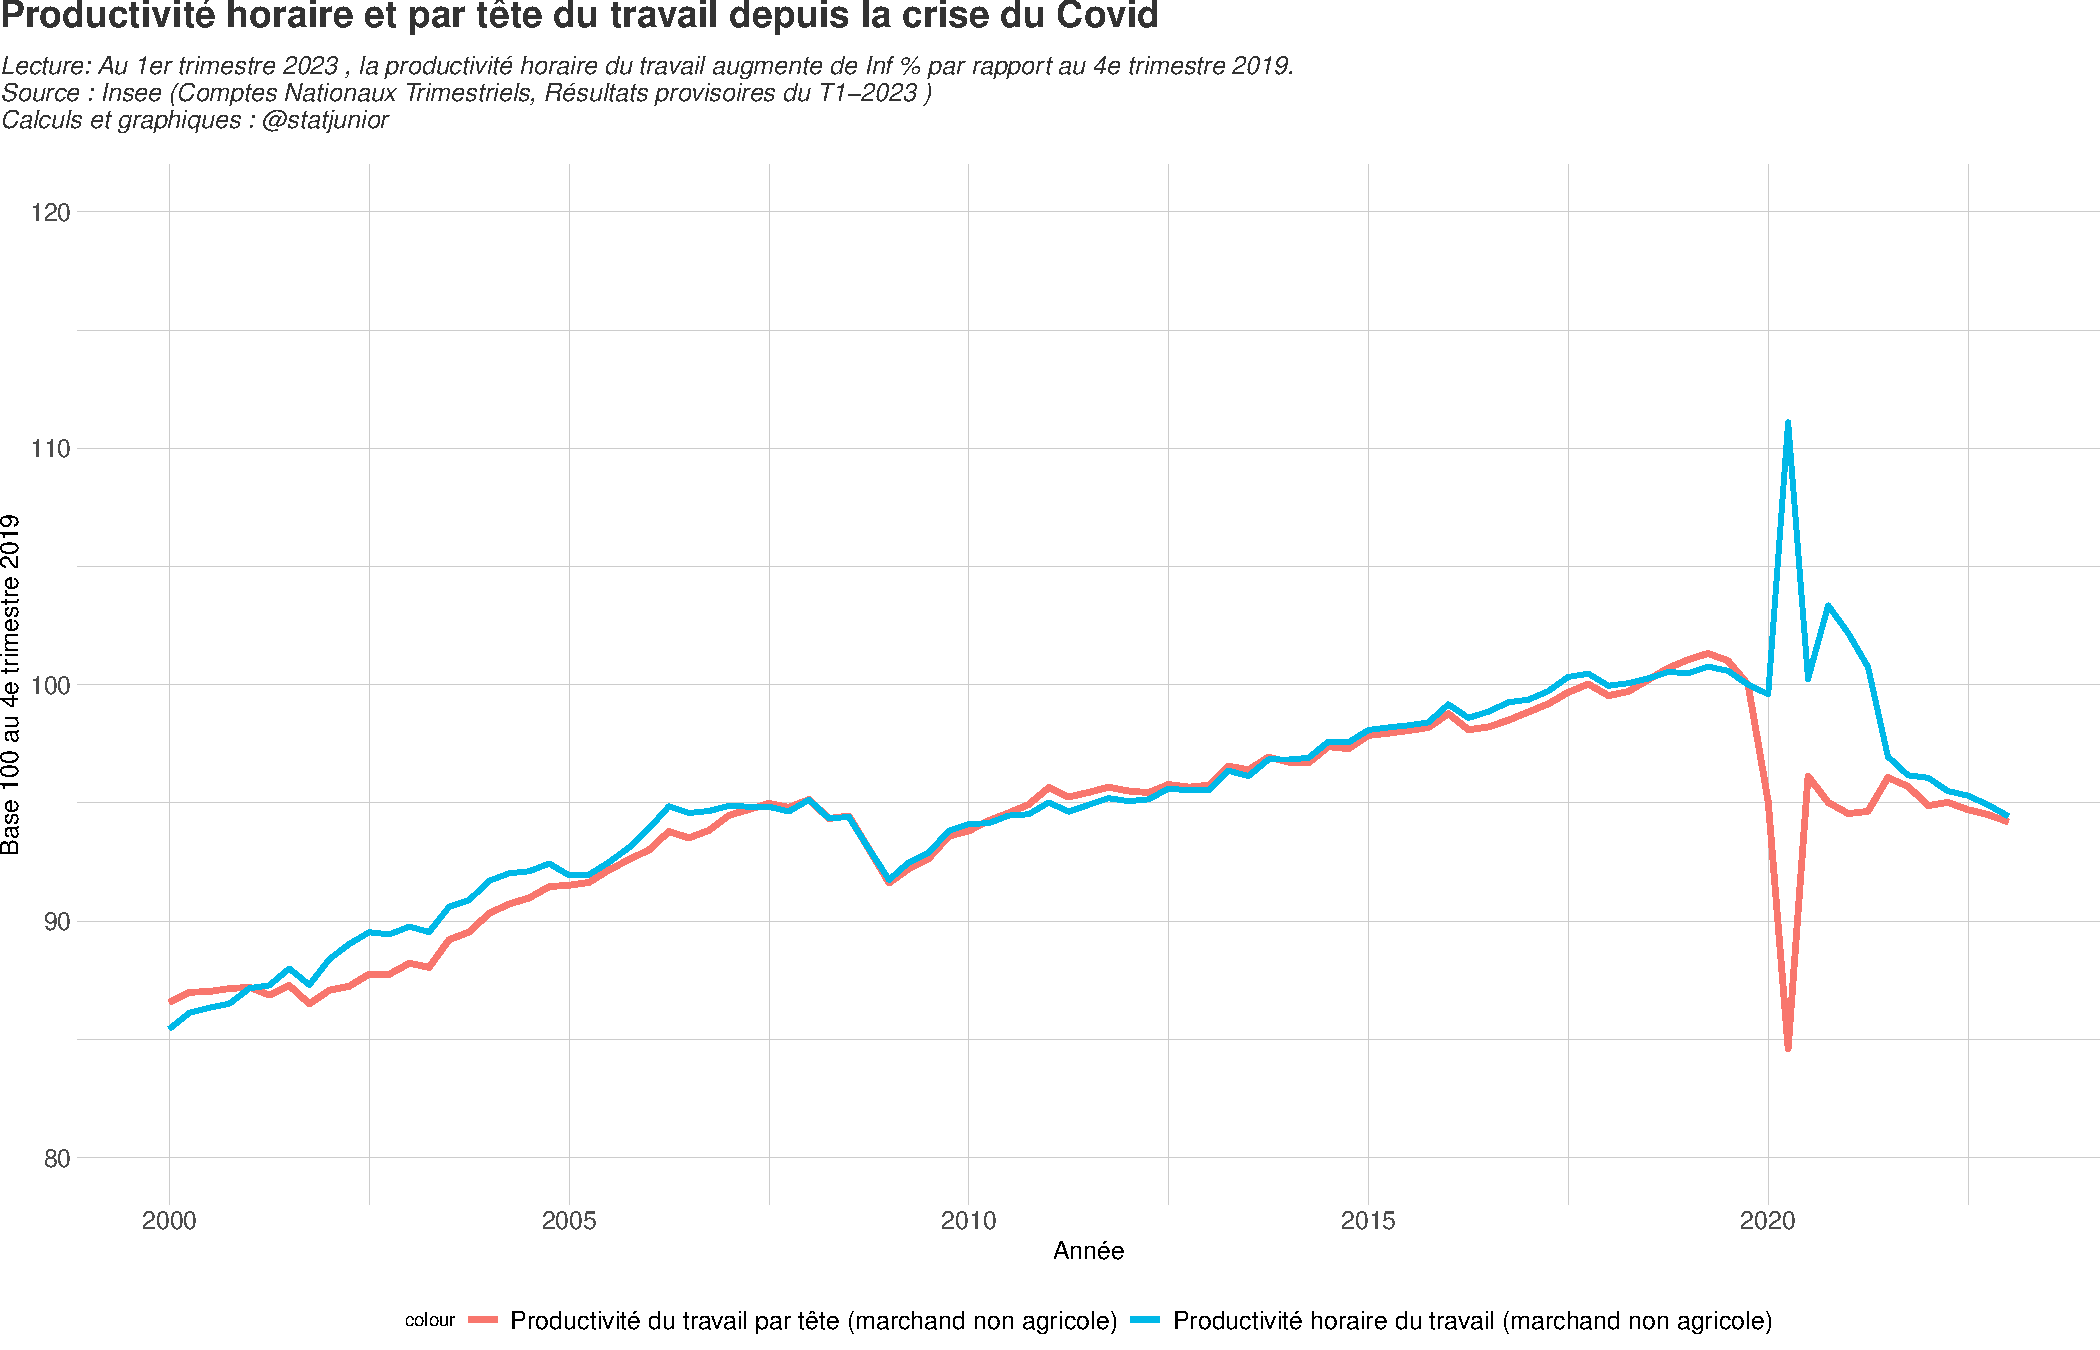
\includegraphics{rapport_pdf_compte_branche_files/figure-latex/unnamed-chunk-12-1.pdf}

\hypertarget{evolution-de-la-masse-salariale-ruxe9elle-et-de-lemploi-depuis-2017}{%
\subsection{Evolution de la masse salariale réelle et de l'emploi depuis
2017}\label{evolution-de-la-masse-salariale-ruxe9elle-et-de-lemploi-depuis-2017}}

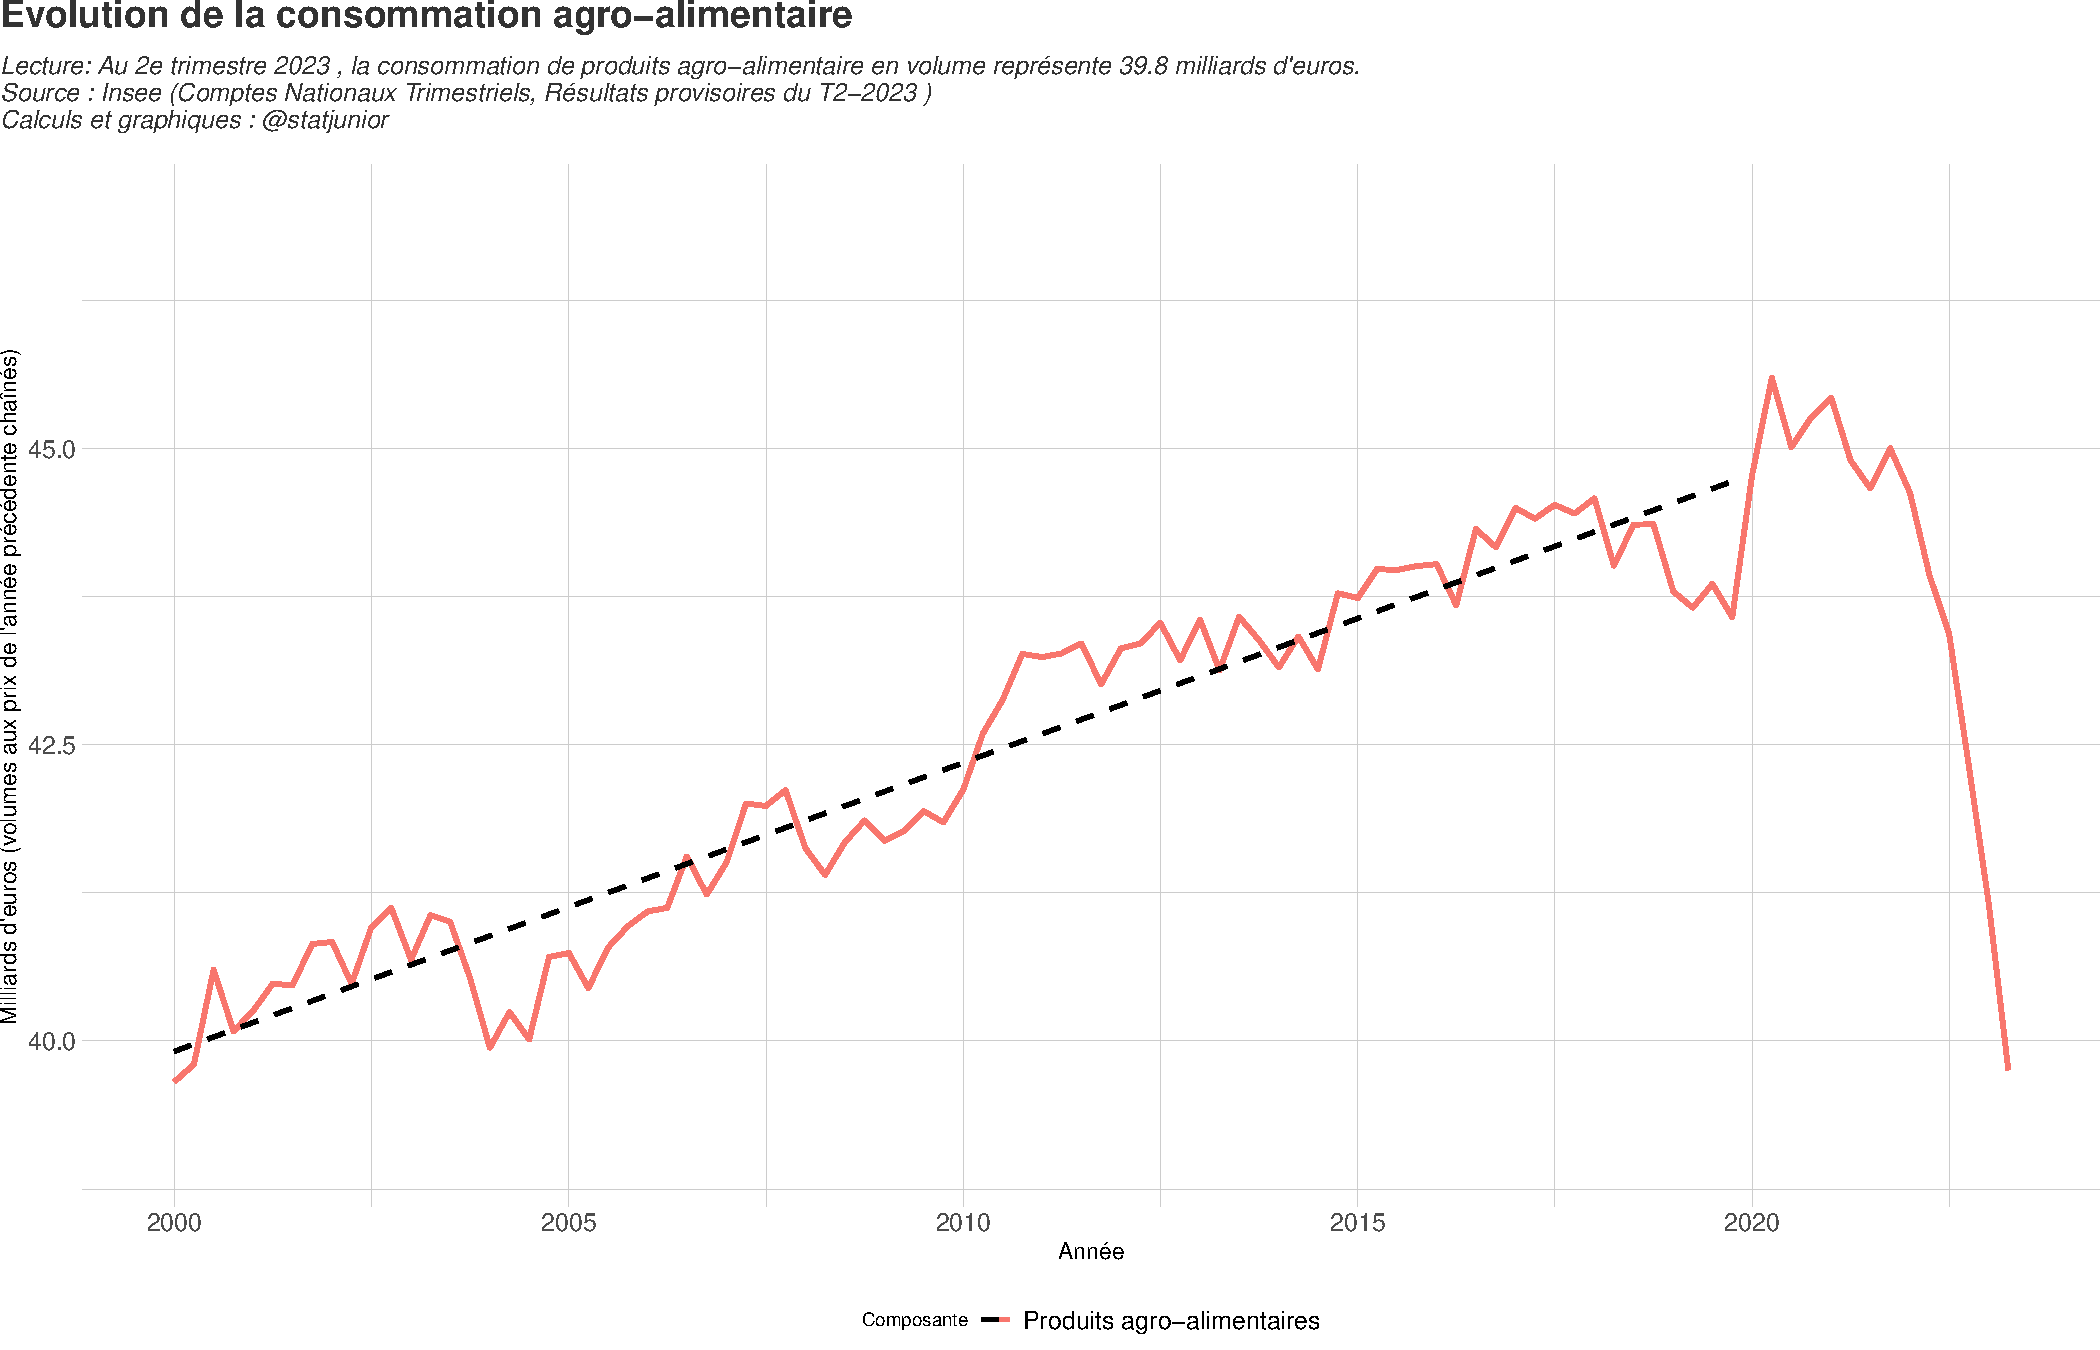
\includegraphics{rapport_pdf_compte_branche_files/figure-latex/unnamed-chunk-13-1.pdf}

\hypertarget{volume-de-travail-global-et-productivituxe9-du-travail-depuis-1990}{%
\subsection{Volume de travail global et productivité du travail depuis
1990}\label{volume-de-travail-global-et-productivituxe9-du-travail-depuis-1990}}

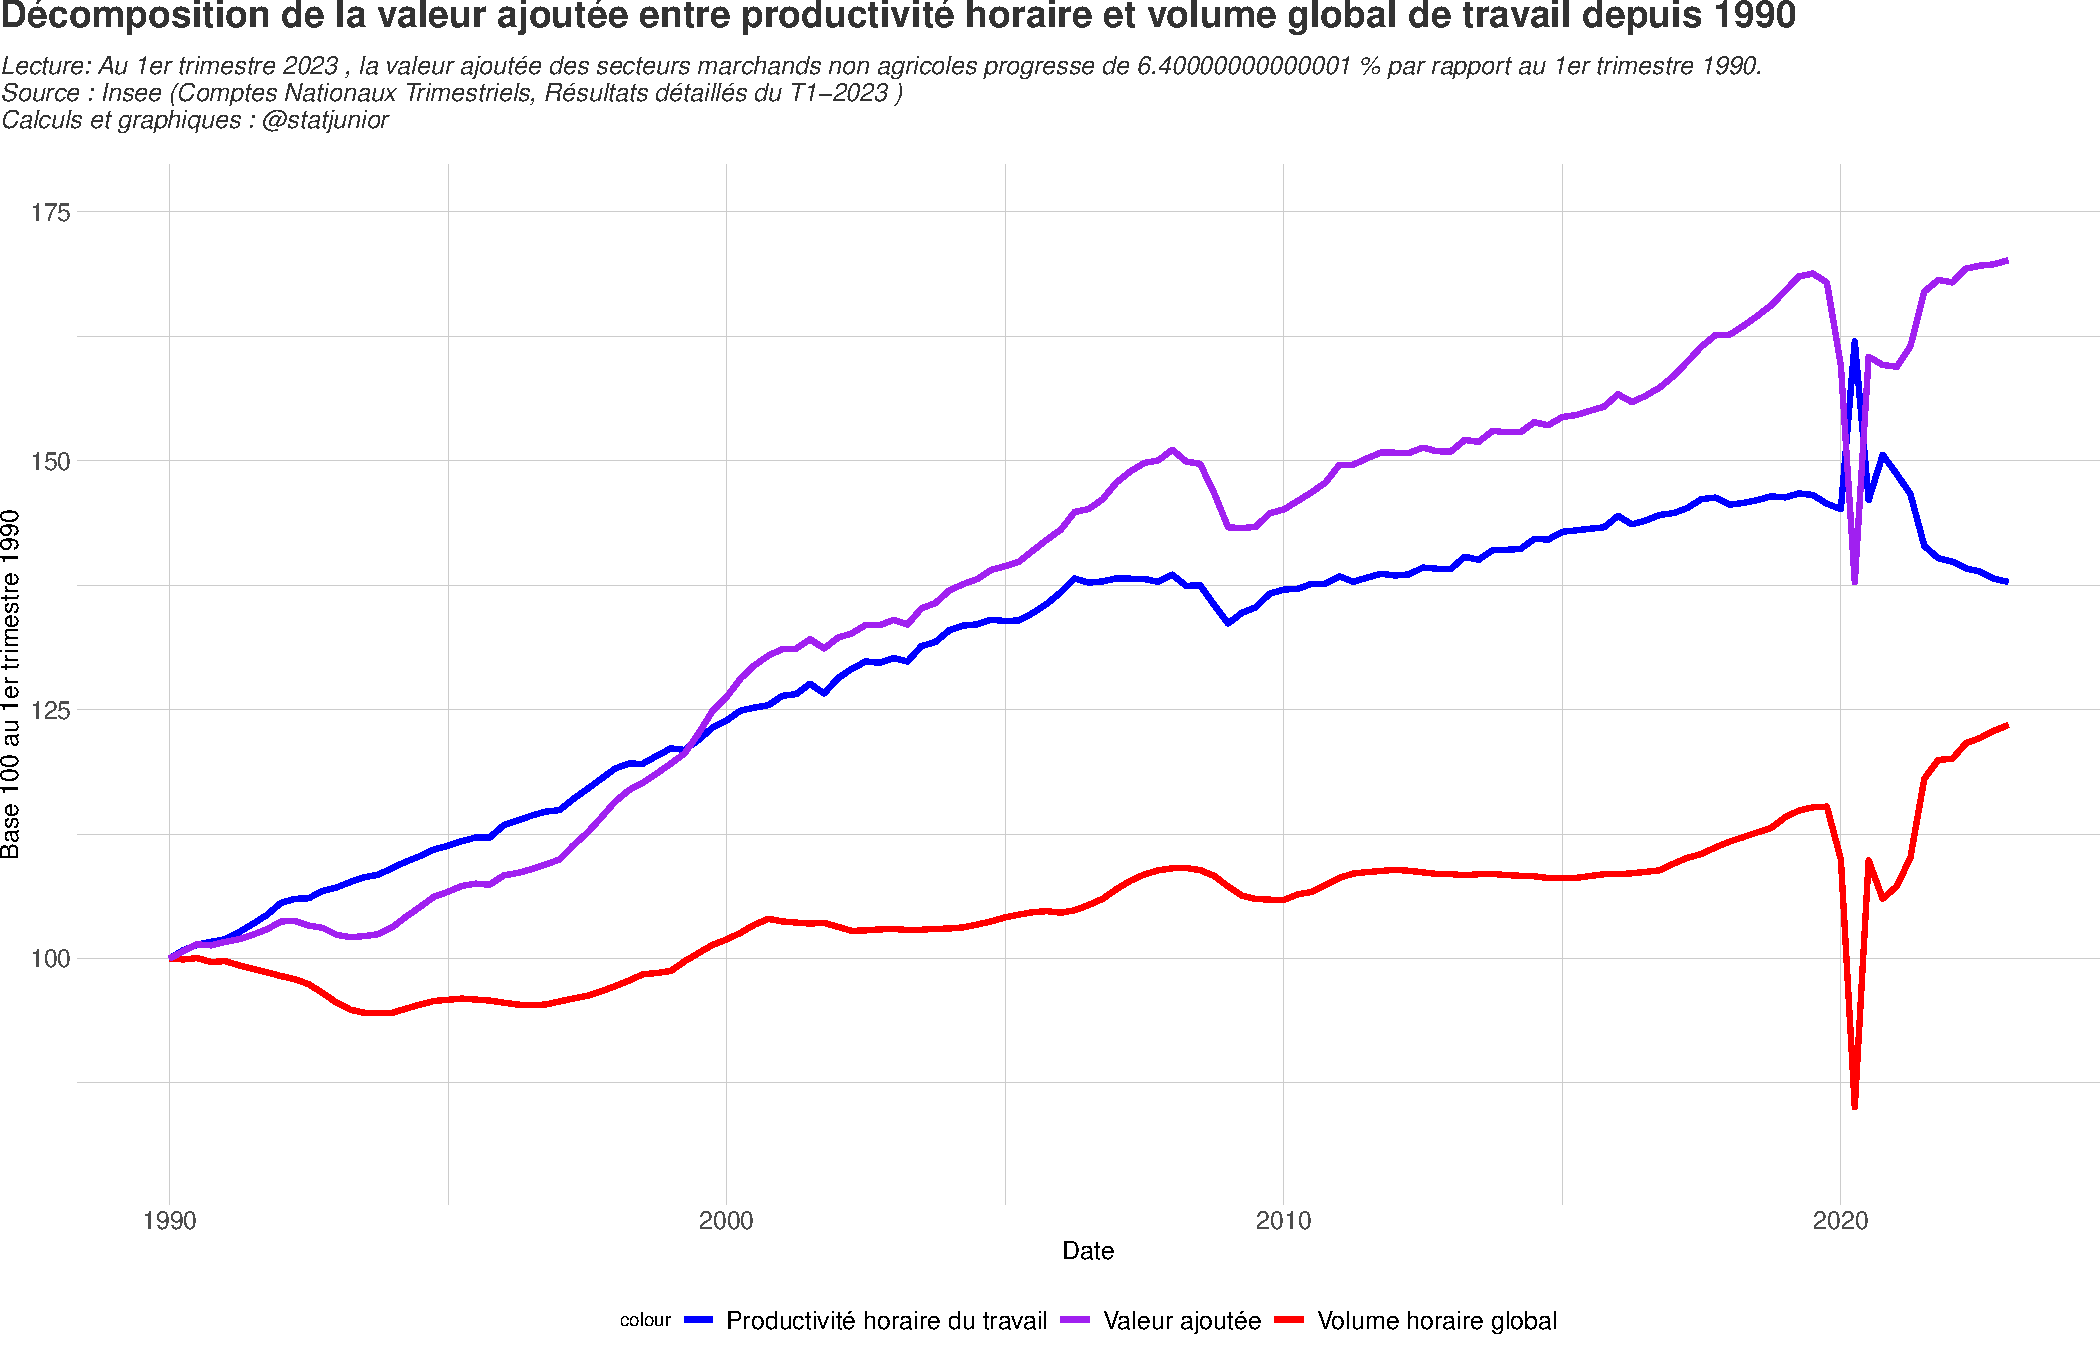
\includegraphics{rapport_pdf_compte_branche_files/figure-latex/unnamed-chunk-14-1.pdf}

\hypertarget{evolution-du-salaire-moyen-par-tuxeate-et-de-la-productivituxe9-par-tuxeate-depuis-1990}{%
\subsection{Evolution du Salaire Moyen par Tête et de la Productivité
par tête depuis
1990}\label{evolution-du-salaire-moyen-par-tuxeate-et-de-la-productivituxe9-par-tuxeate-depuis-1990}}

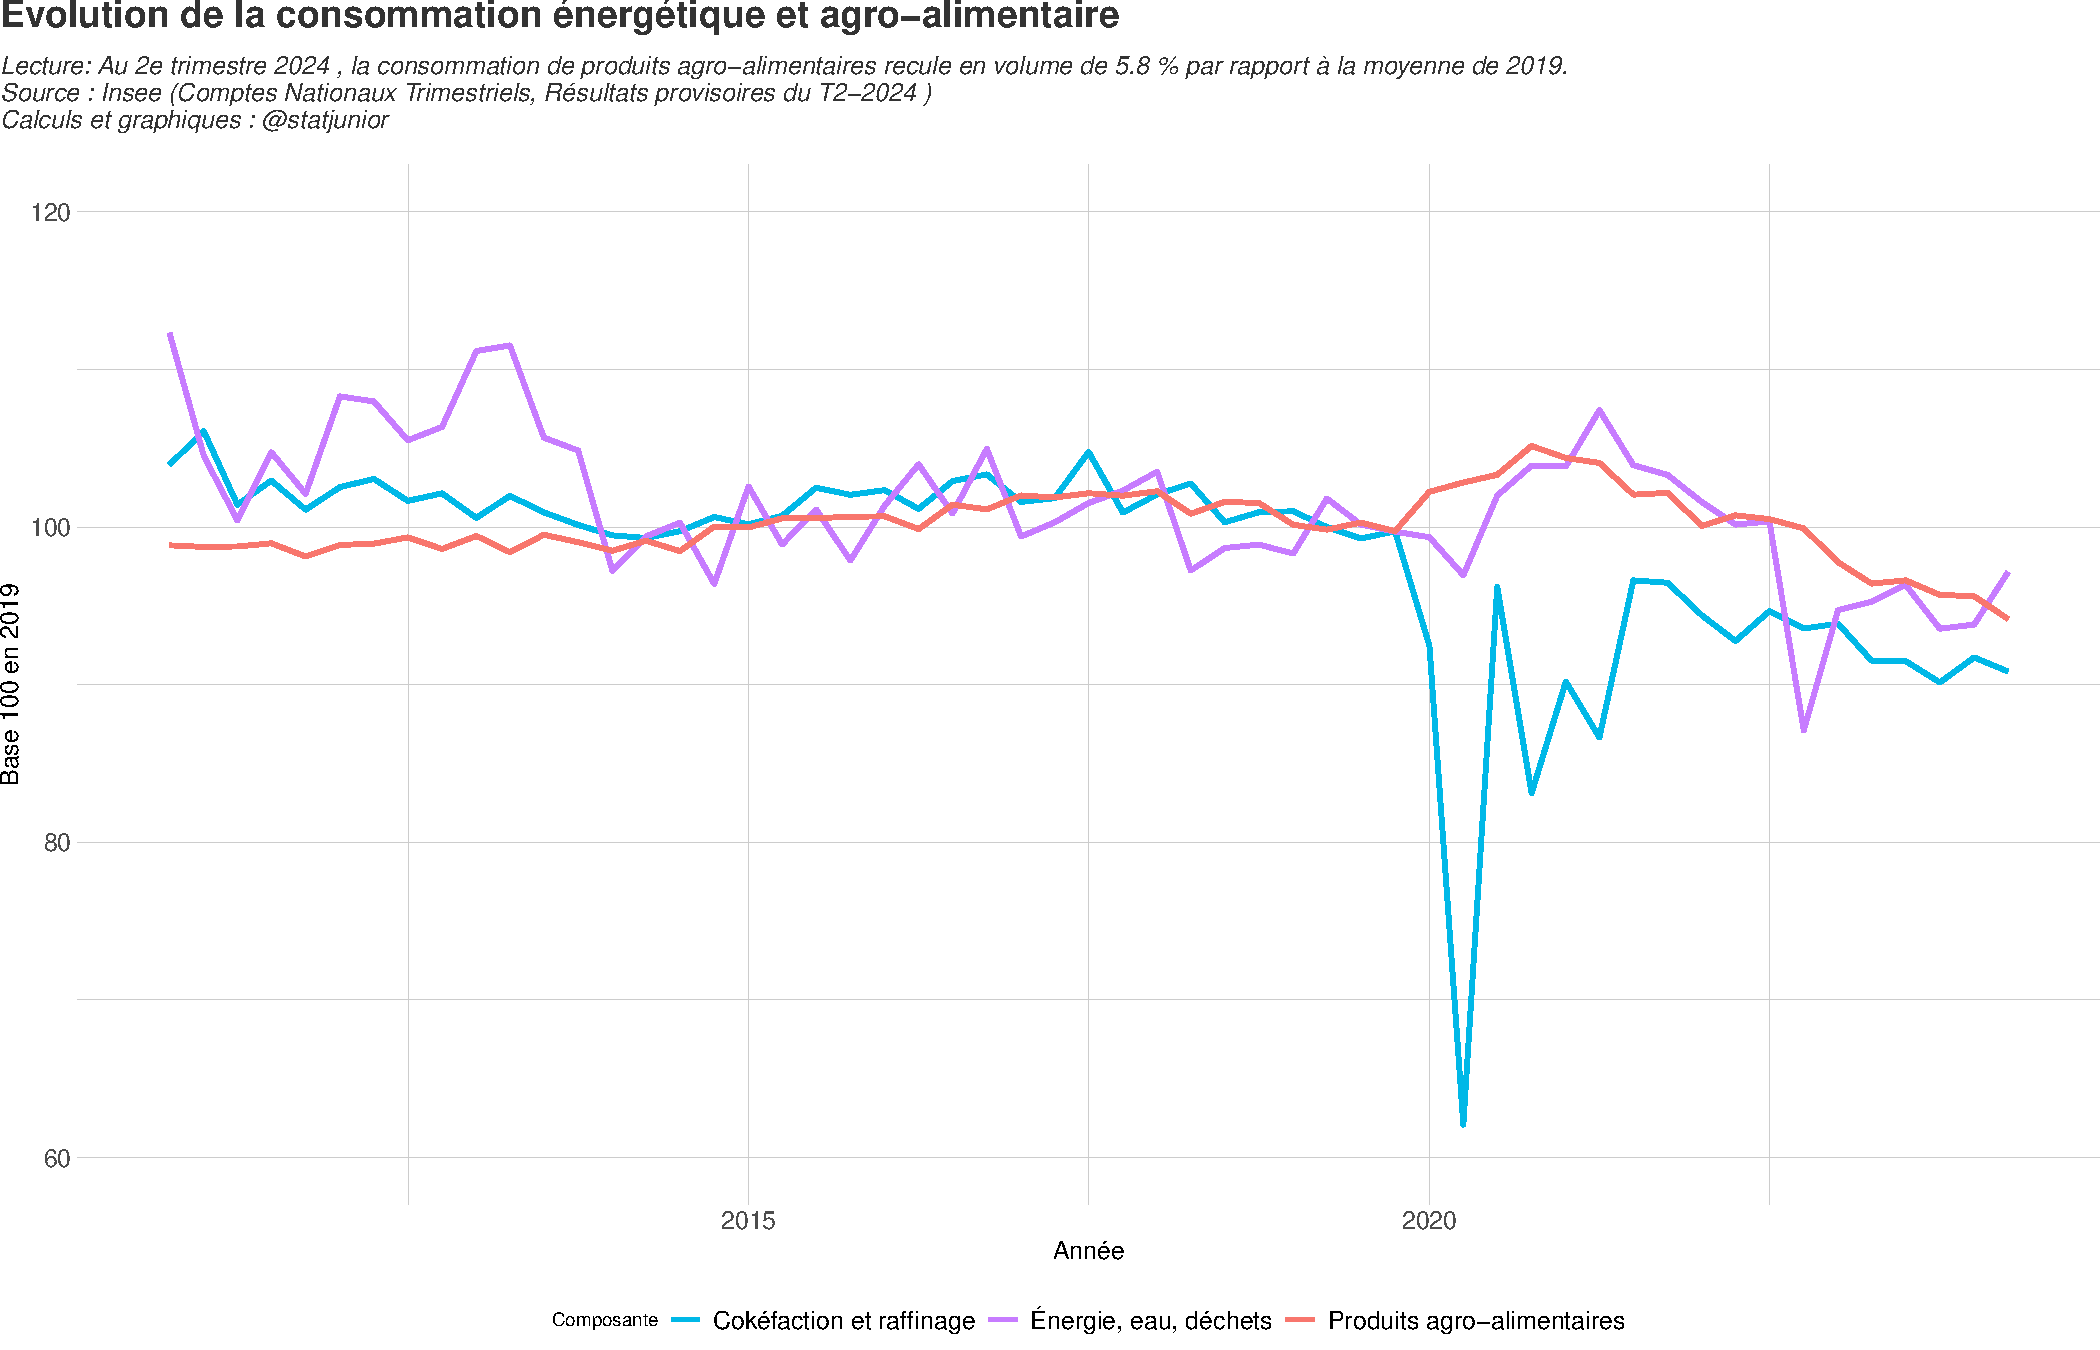
\includegraphics{rapport_pdf_compte_branche_files/figure-latex/unnamed-chunk-15-1.pdf}

\newpage

\hypertarget{duxe9composition-des-agruxe9gats-macoruxe9conomiques-par-branche-dactivituxe9}{%
\section{Décomposition des agrégats macoréconomiques par branche
d'activité}\label{duxe9composition-des-agruxe9gats-macoruxe9conomiques-par-branche-dactivituxe9}}

\hypertarget{valeur-ajoutuxe9e-par-branche-depuis-fin-2019}{%
\subsection{Valeur ajoutée par branche depuis fin
2019}\label{valeur-ajoutuxe9e-par-branche-depuis-fin-2019}}

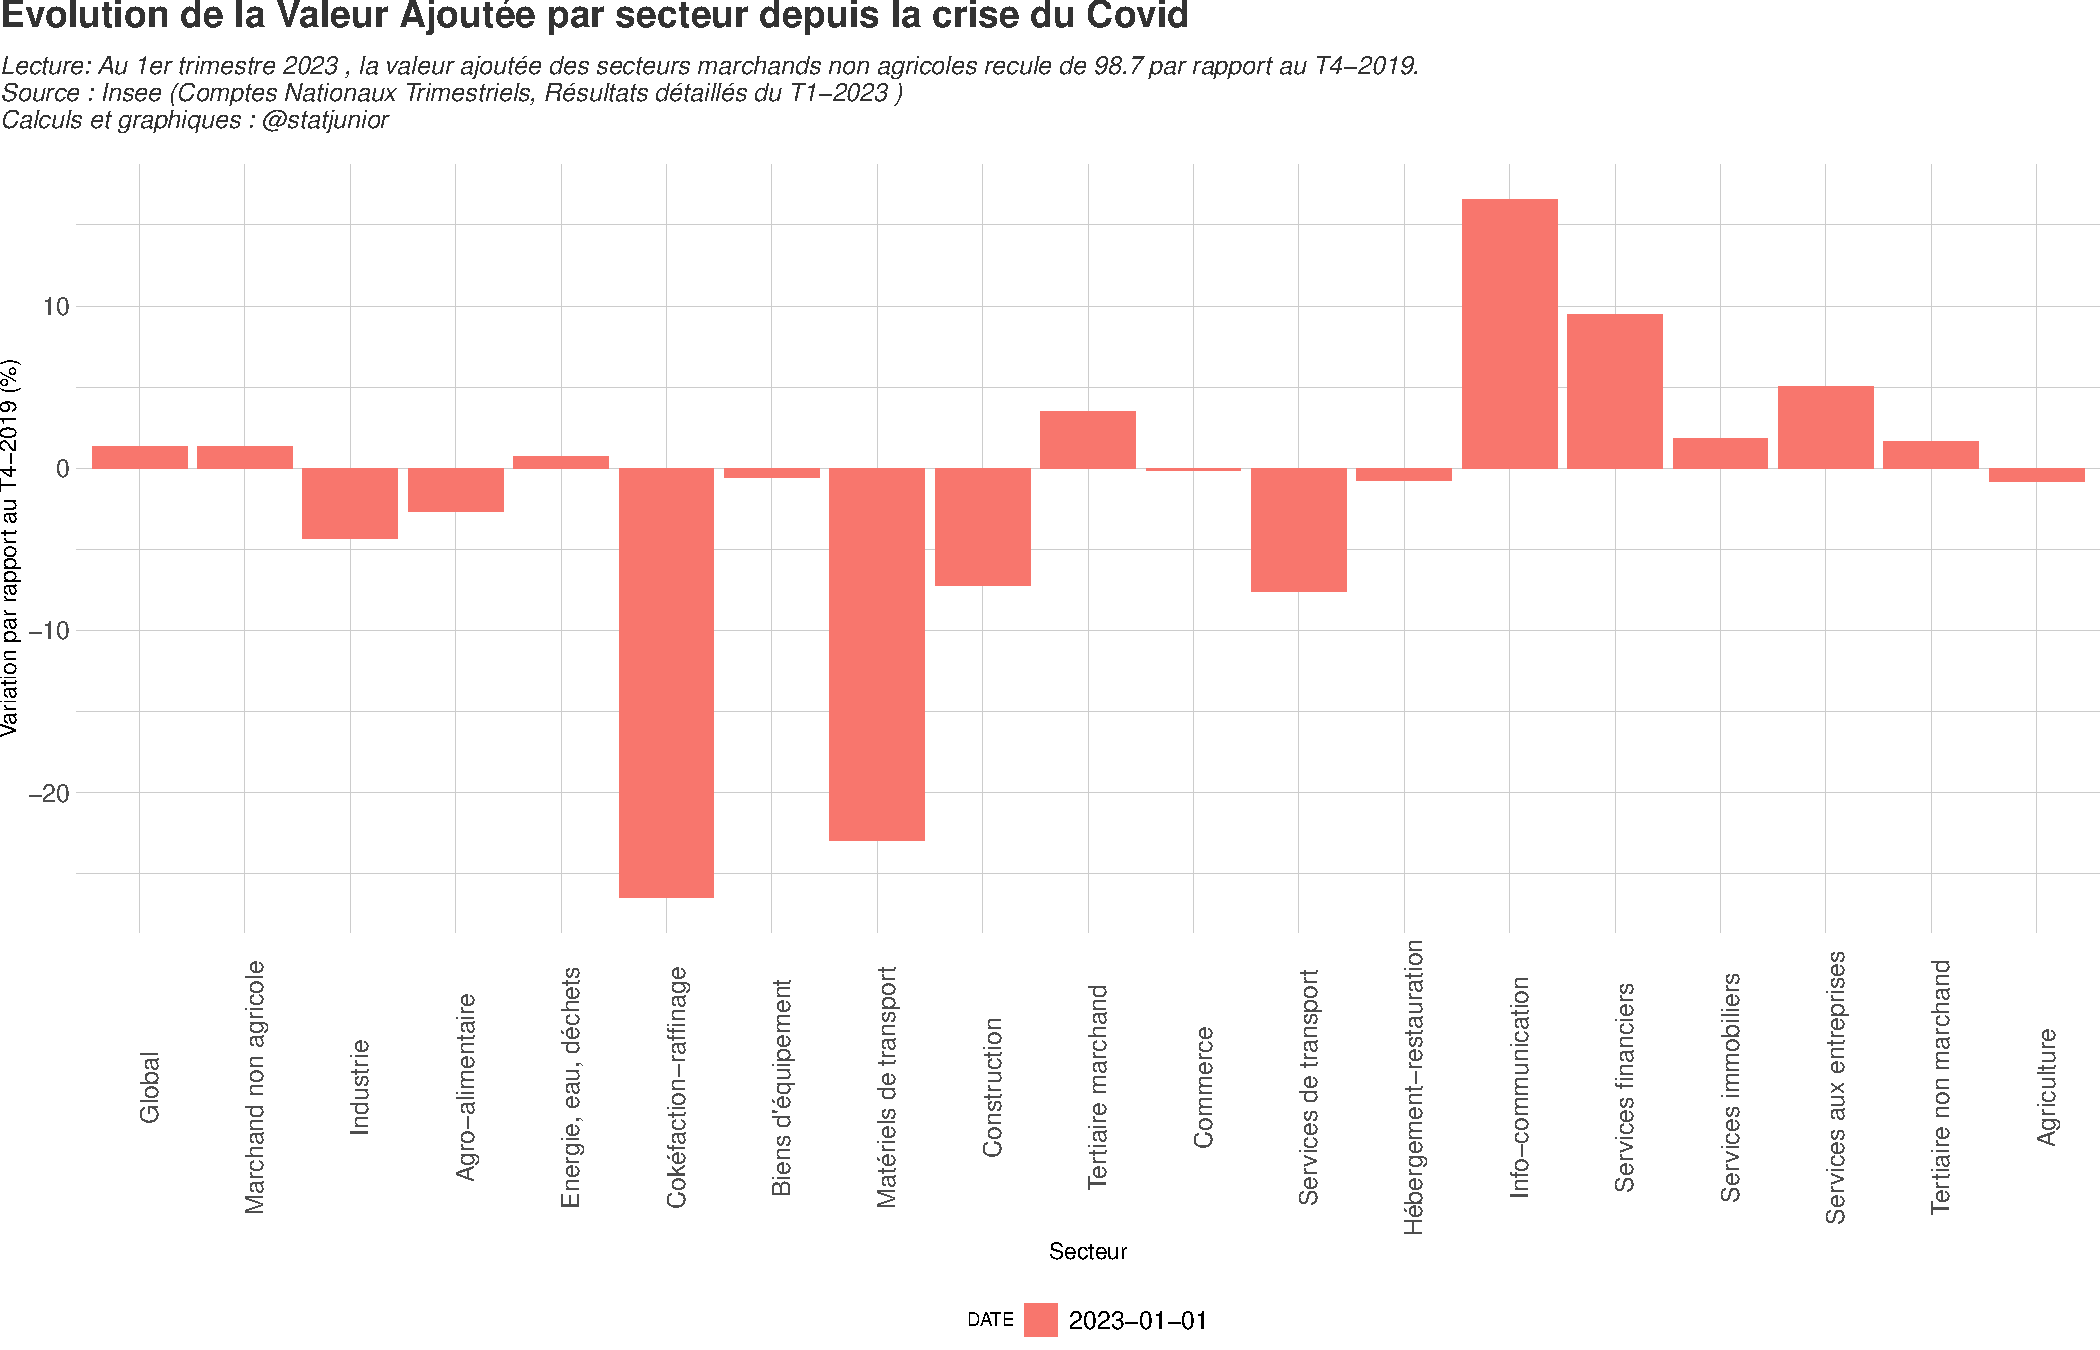
\includegraphics{rapport_pdf_compte_branche_files/figure-latex/unnamed-chunk-16-1.pdf}

\hypertarget{progression-de-la-valeur-ajoutuxe9e-par-rapport-au-dernier-trimestre}{%
\subsection{Progression de la valeur ajoutée par rapport au dernier
trimestre}\label{progression-de-la-valeur-ajoutuxe9e-par-rapport-au-dernier-trimestre}}

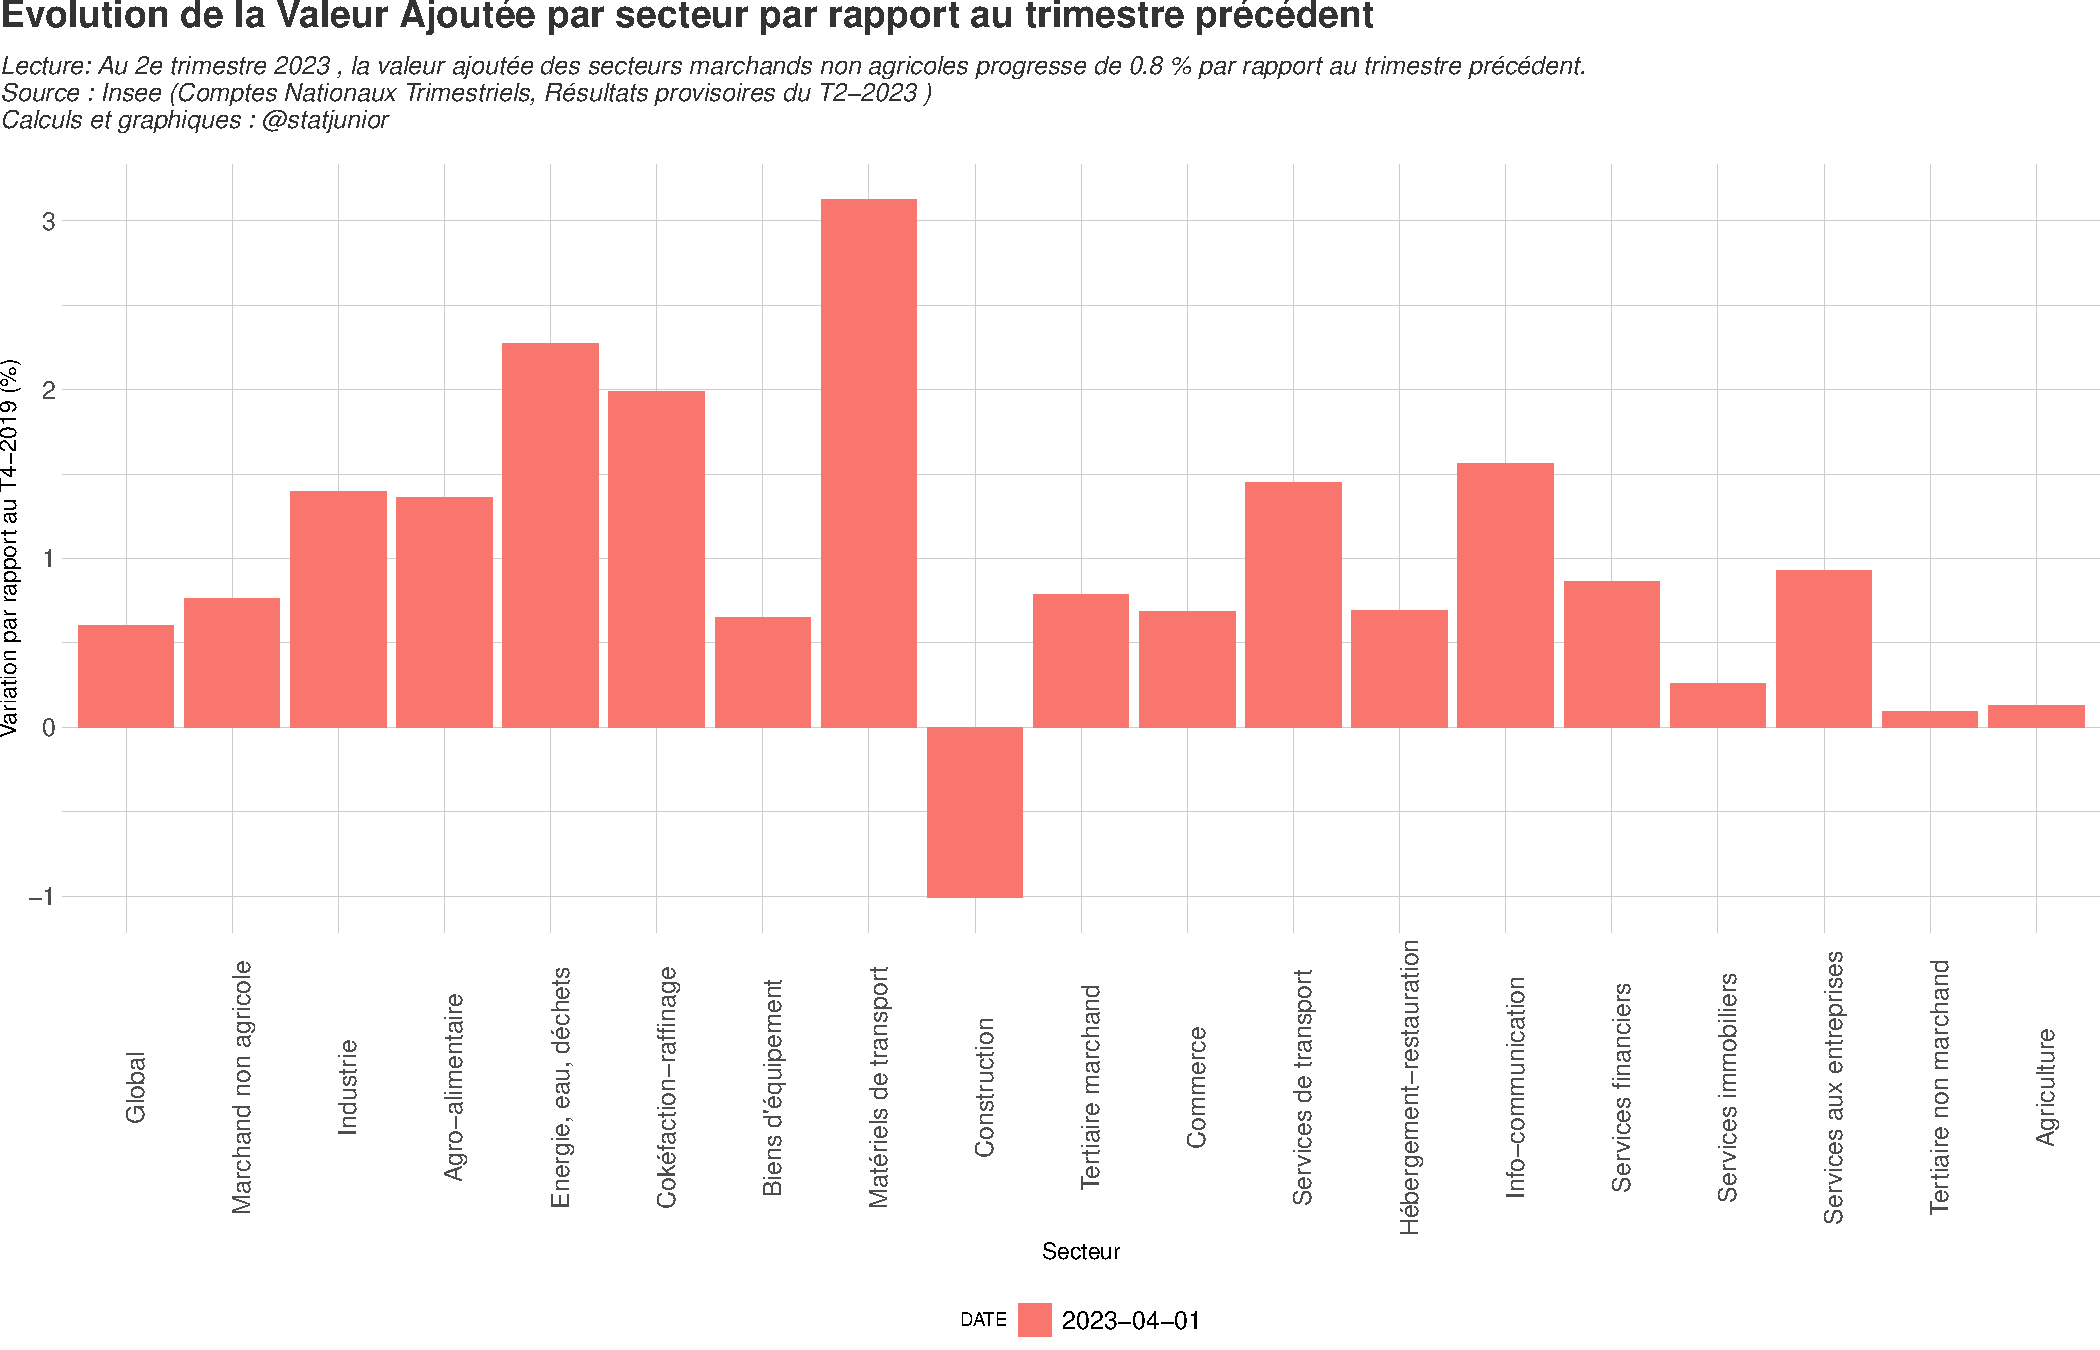
\includegraphics{rapport_pdf_compte_branche_files/figure-latex/unnamed-chunk-17-1.pdf}

\hypertarget{productivituxe9-du-travail-sectorielle-depuis-2019}{%
\subsection{Productivité du travail sectorielle depuis
2019}\label{productivituxe9-du-travail-sectorielle-depuis-2019}}

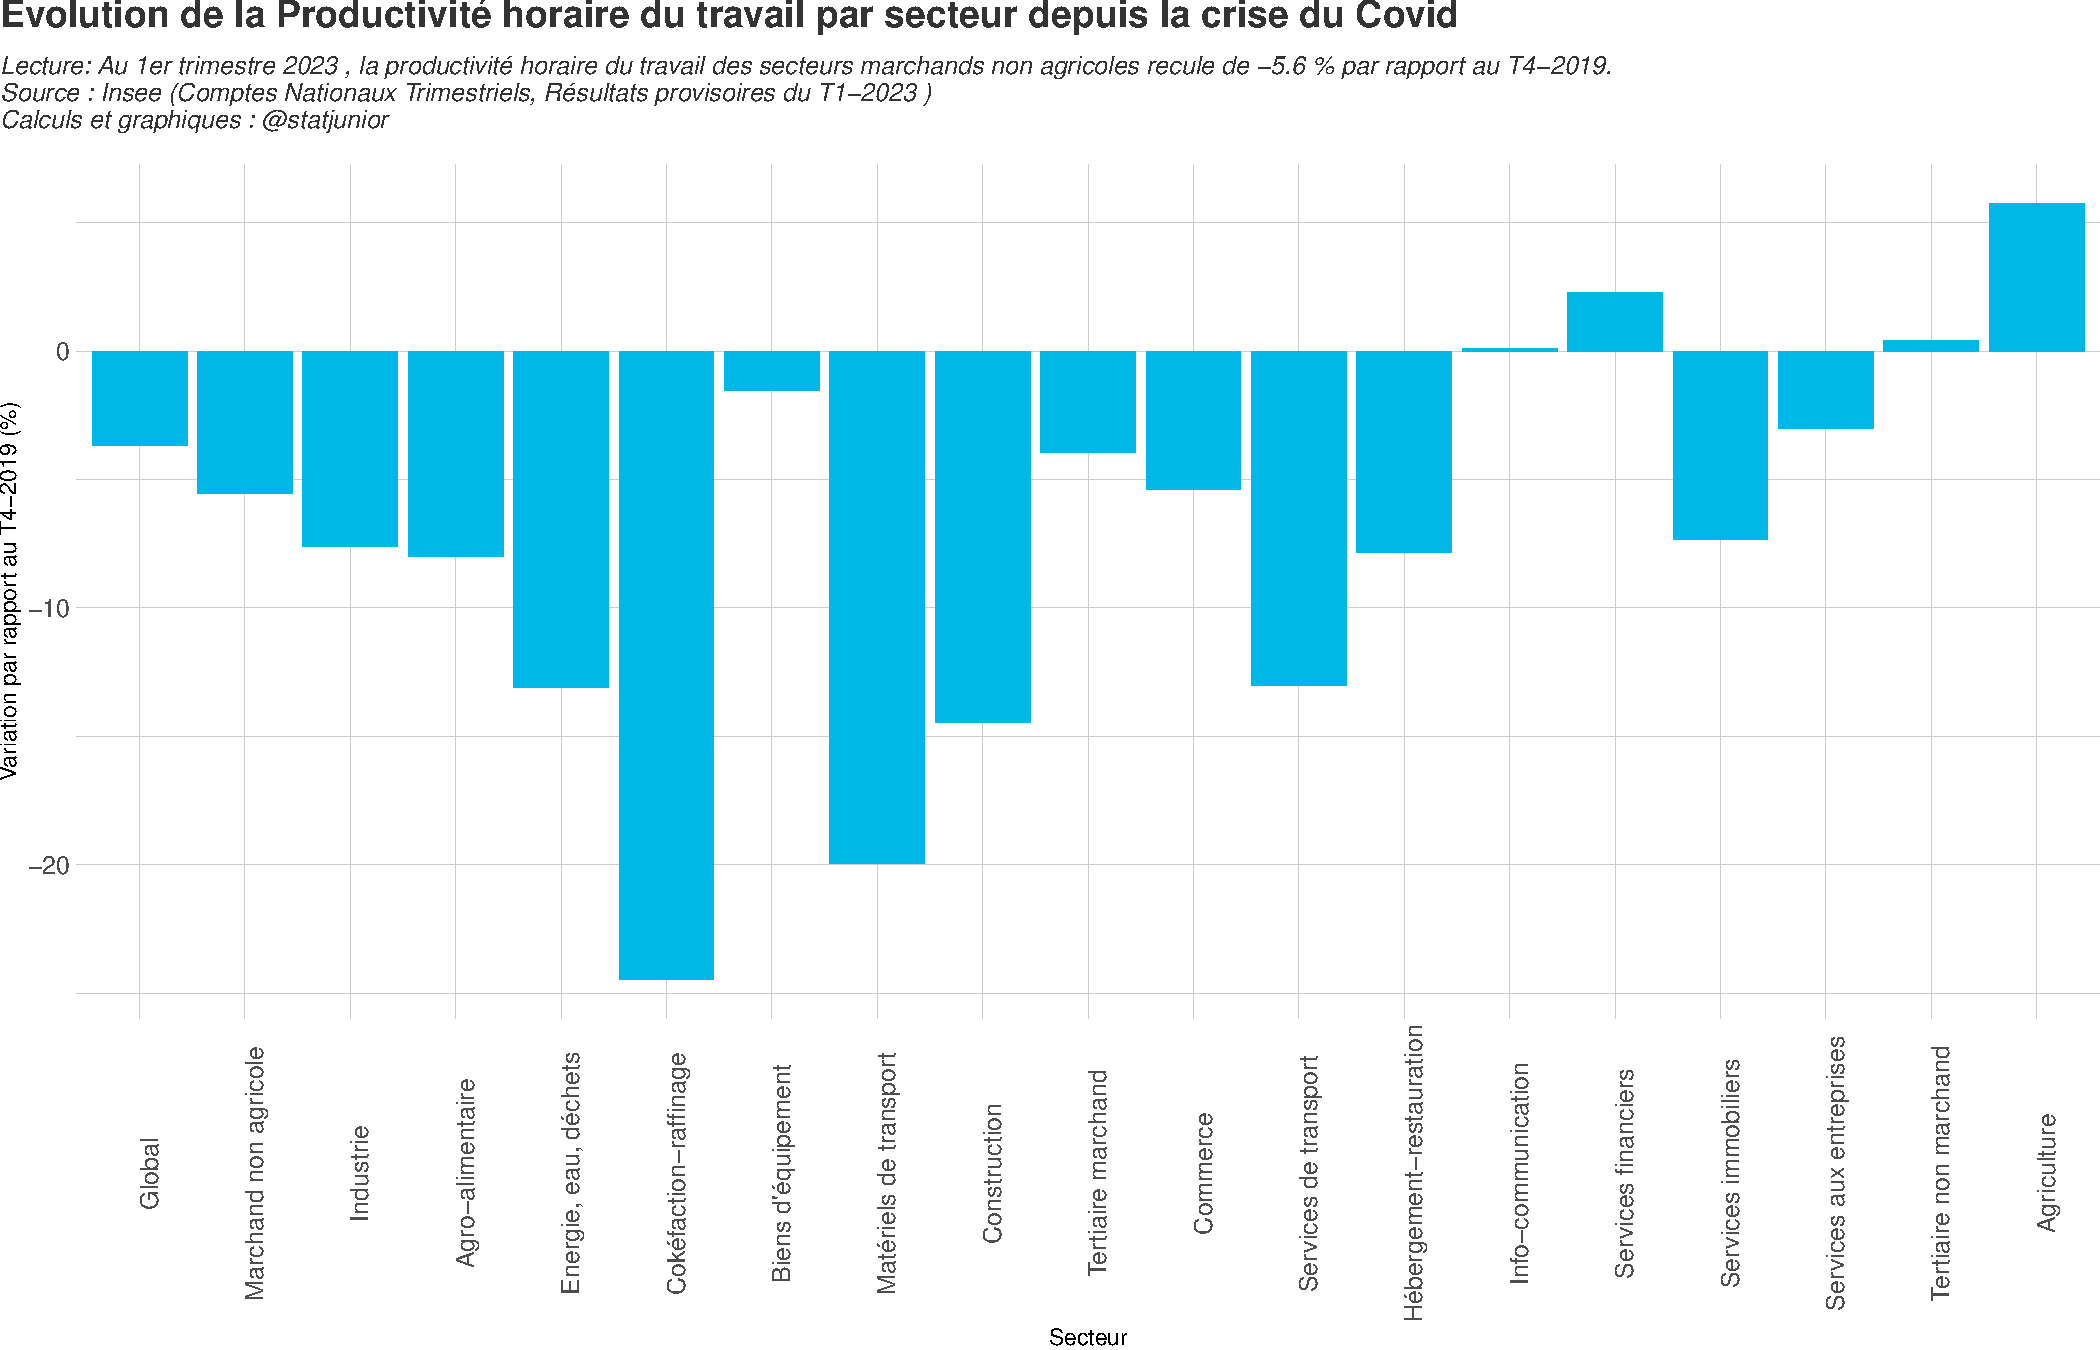
\includegraphics{rapport_pdf_compte_branche_files/figure-latex/unnamed-chunk-18-1.pdf}

\hypertarget{evolution-du-volume-dheures-travailluxe9es-par-branche-depuis-2019}{%
\subsection{Evolution du volume d'heures travaillées par branche depuis
2019}\label{evolution-du-volume-dheures-travailluxe9es-par-branche-depuis-2019}}

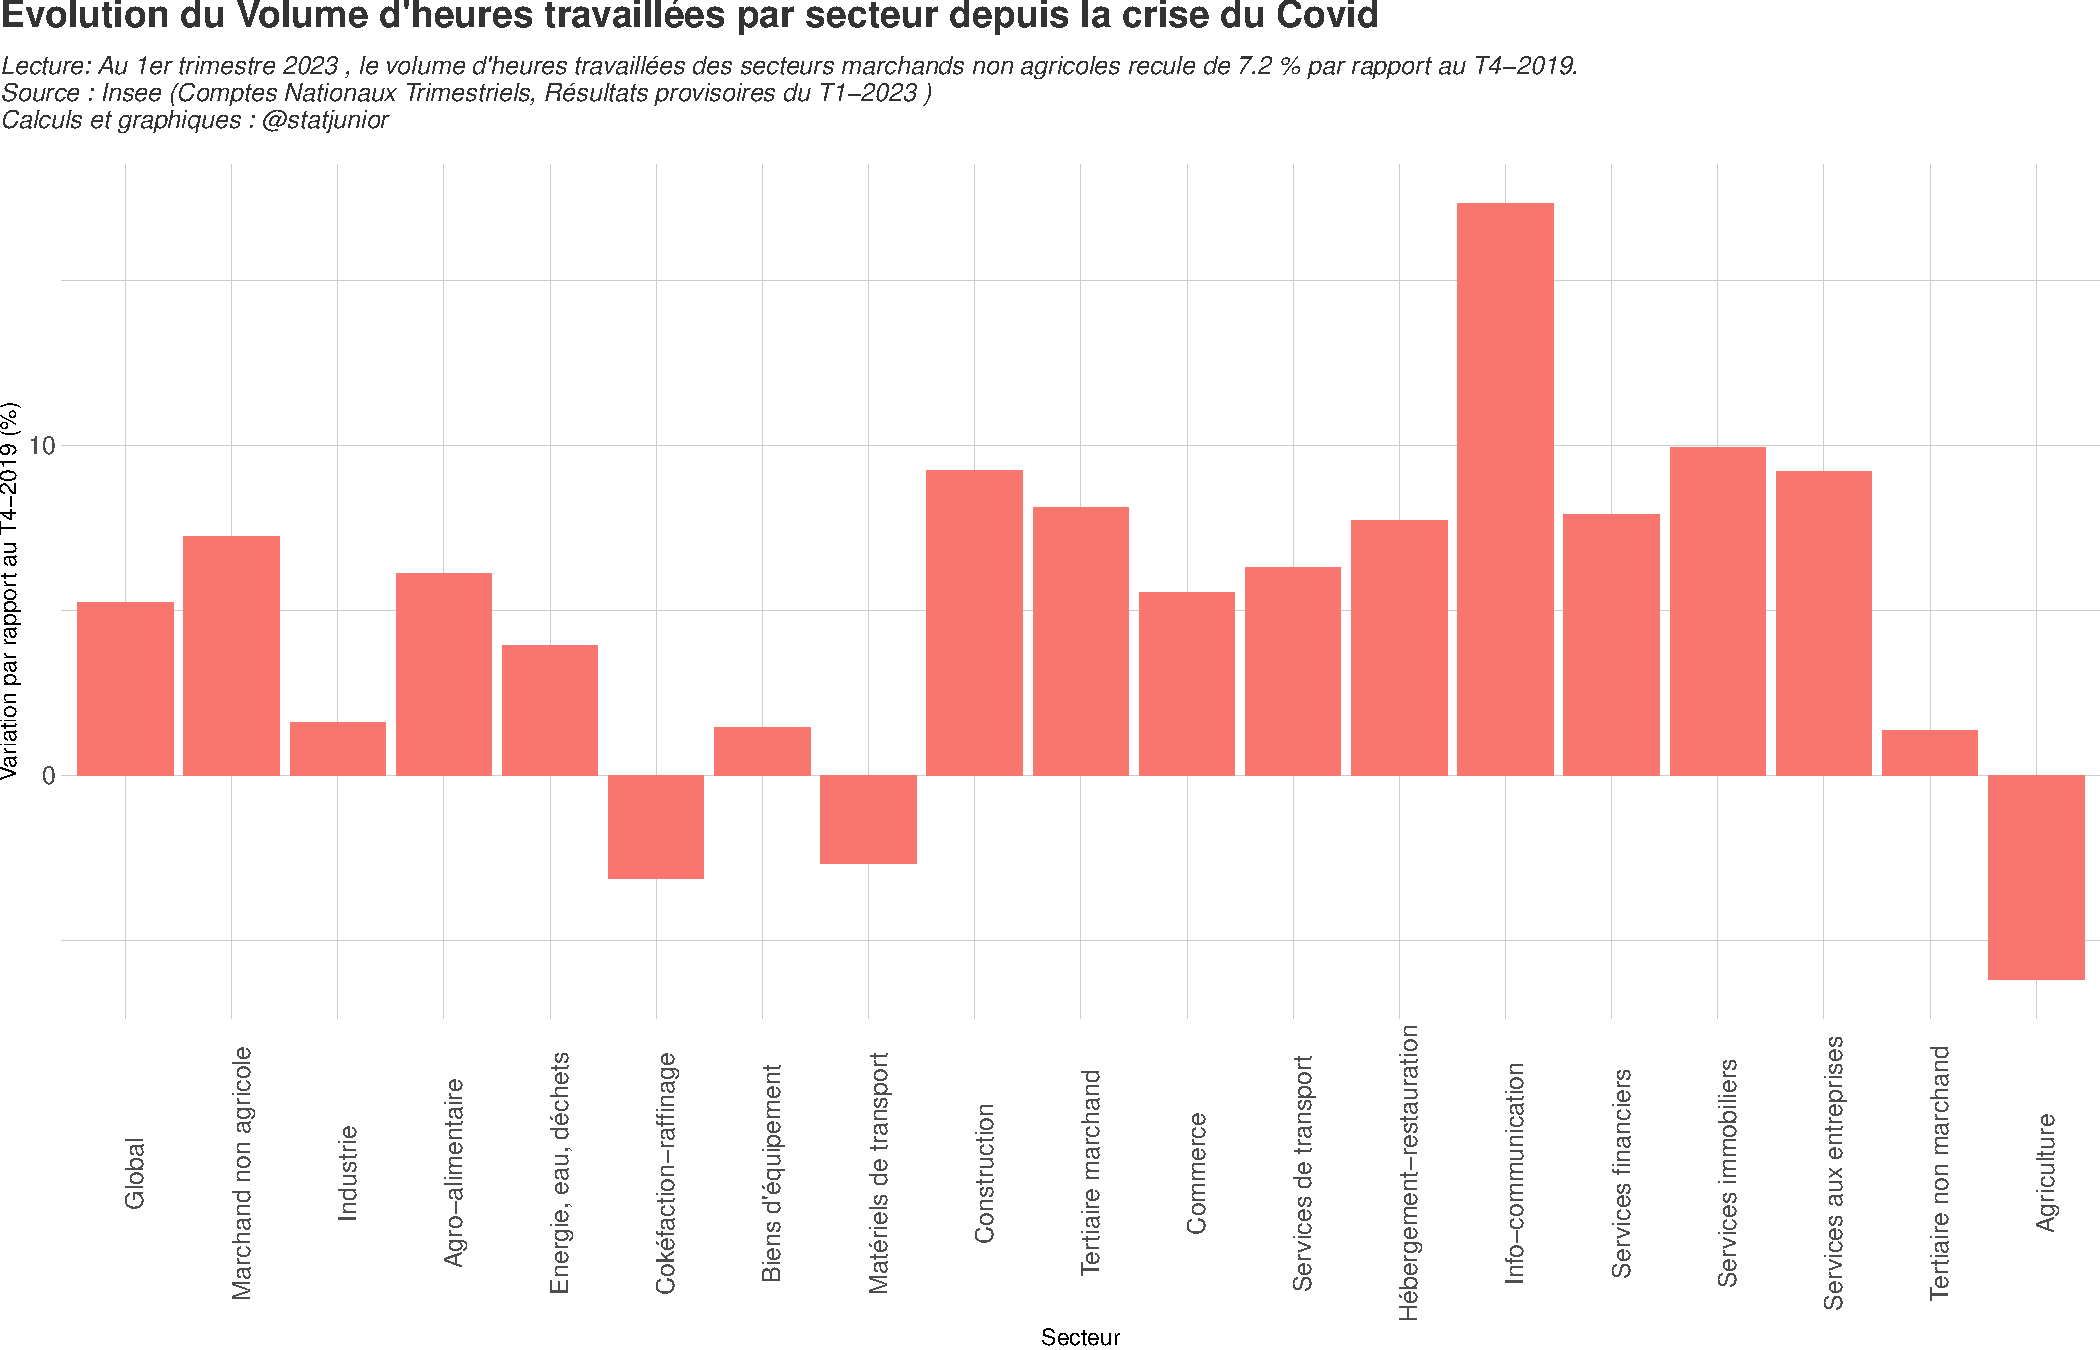
\includegraphics{rapport_pdf_compte_branche_files/figure-latex/unnamed-chunk-19-1.pdf}

\hypertarget{duxe9composition-de-la-productivituxe9-contribution-de-la-valeur-ajoutuxe9e-et-du-volume-dheures-travailluxe9es-par-secteur}{%
\subsection{Décomposition de la Productivité : contribution de la valeur
ajoutée et du volume d'heures travaillées par
secteur}\label{duxe9composition-de-la-productivituxe9-contribution-de-la-valeur-ajoutuxe9e-et-du-volume-dheures-travailluxe9es-par-secteur}}

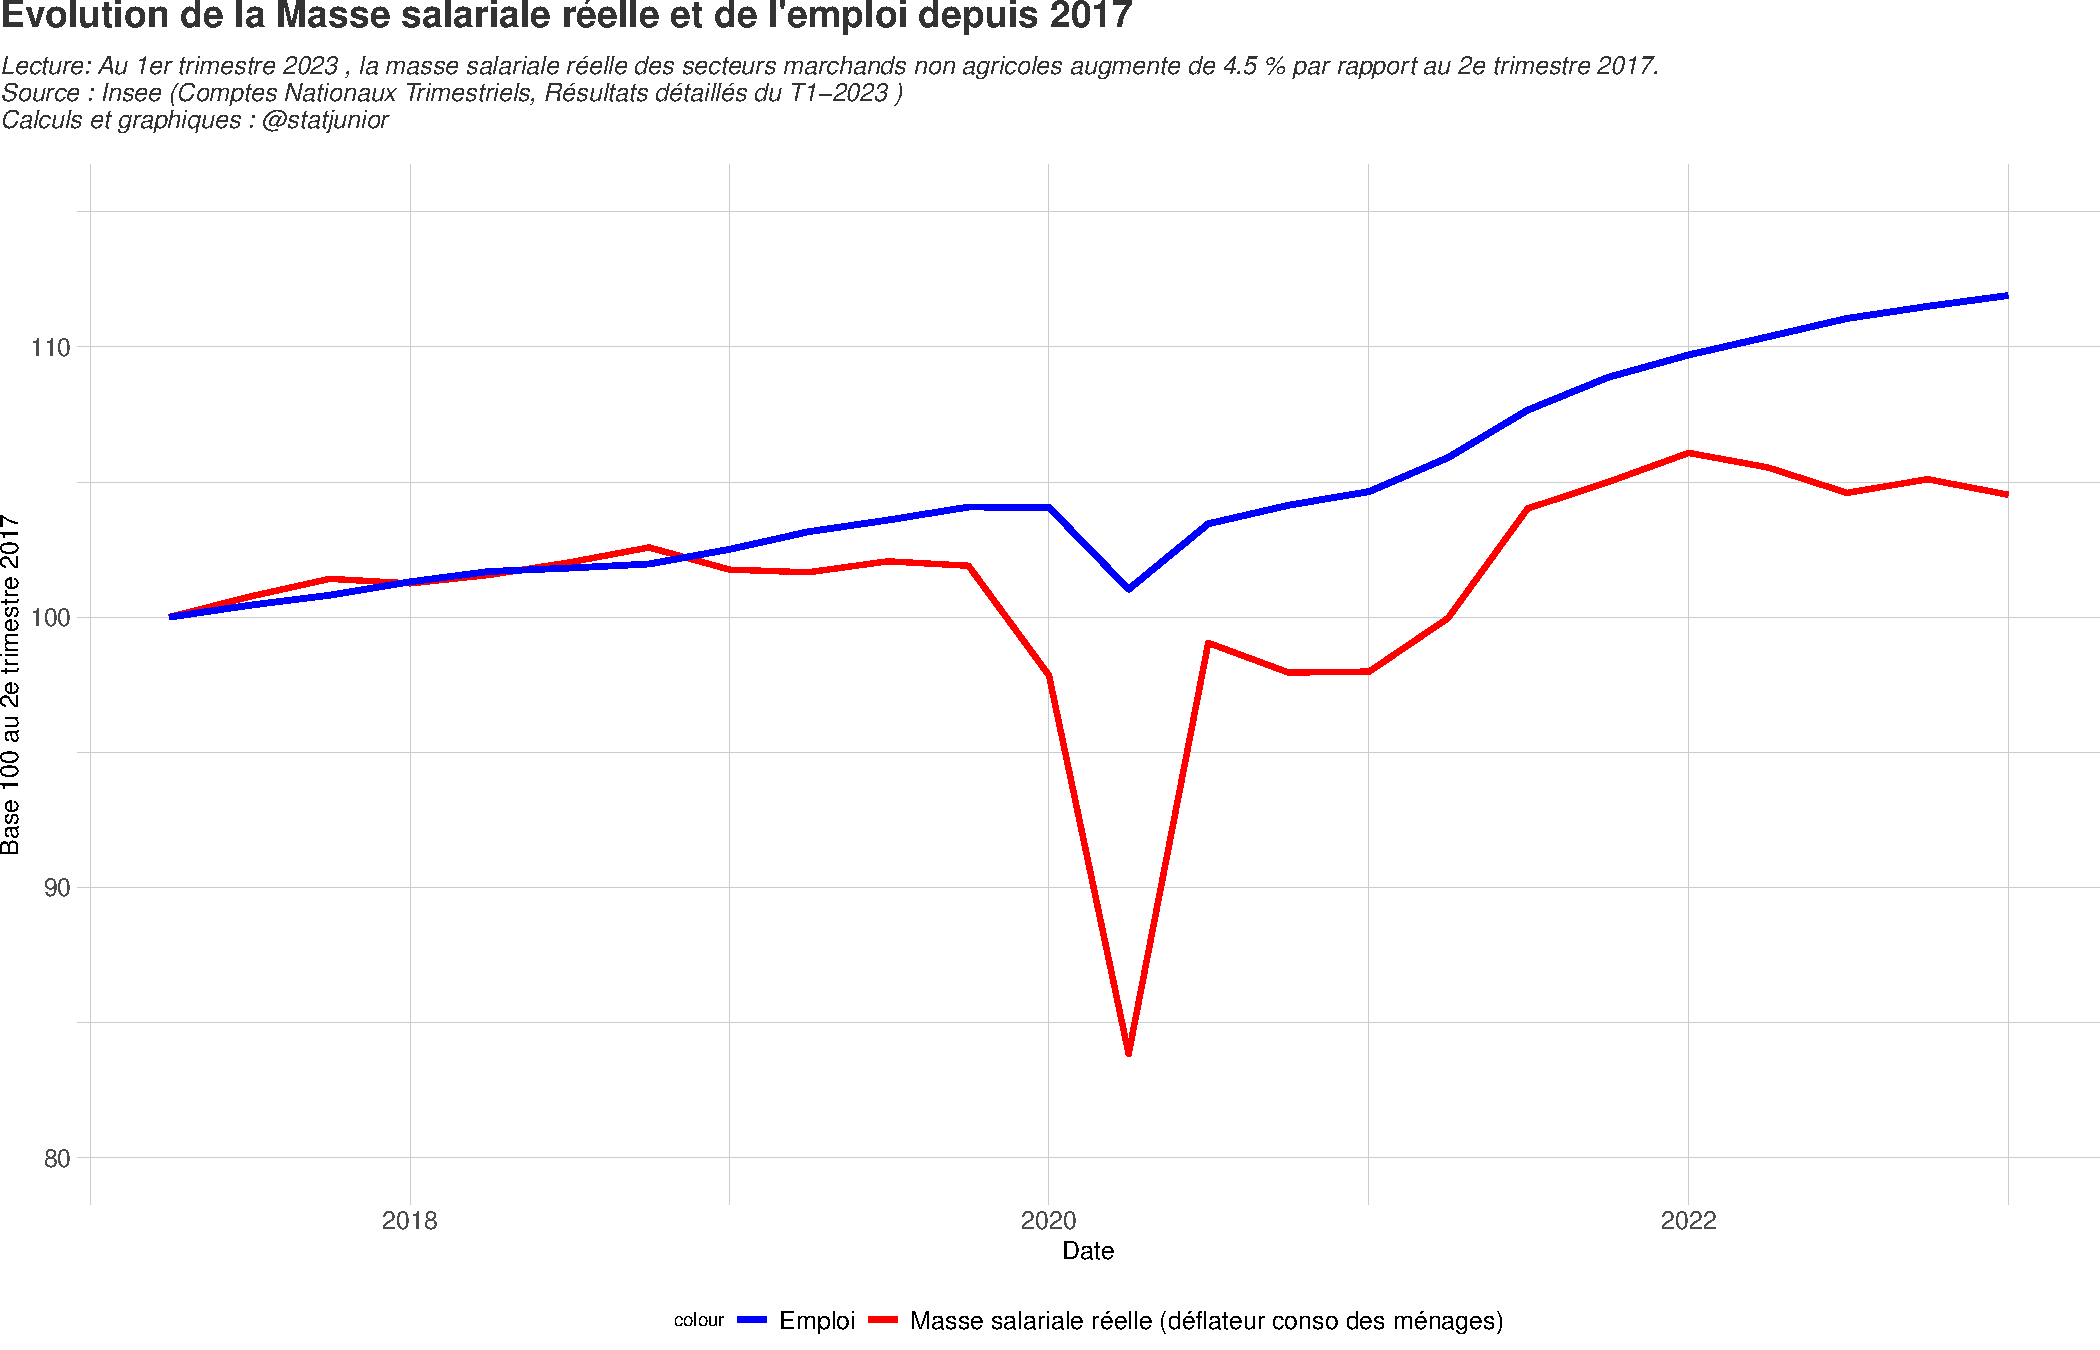
\includegraphics{rapport_pdf_compte_branche_files/figure-latex/unnamed-chunk-20-1.pdf}

\newpage

\hypertarget{taux-de-marge}{%
\section{Taux de marge}\label{taux-de-marge}}

\hypertarget{evolution-du-taux-de-marge-sur-longue-puxe9riode}{%
\subsection{Evolution du taux de marge sur longue
période}\label{evolution-du-taux-de-marge-sur-longue-puxe9riode}}

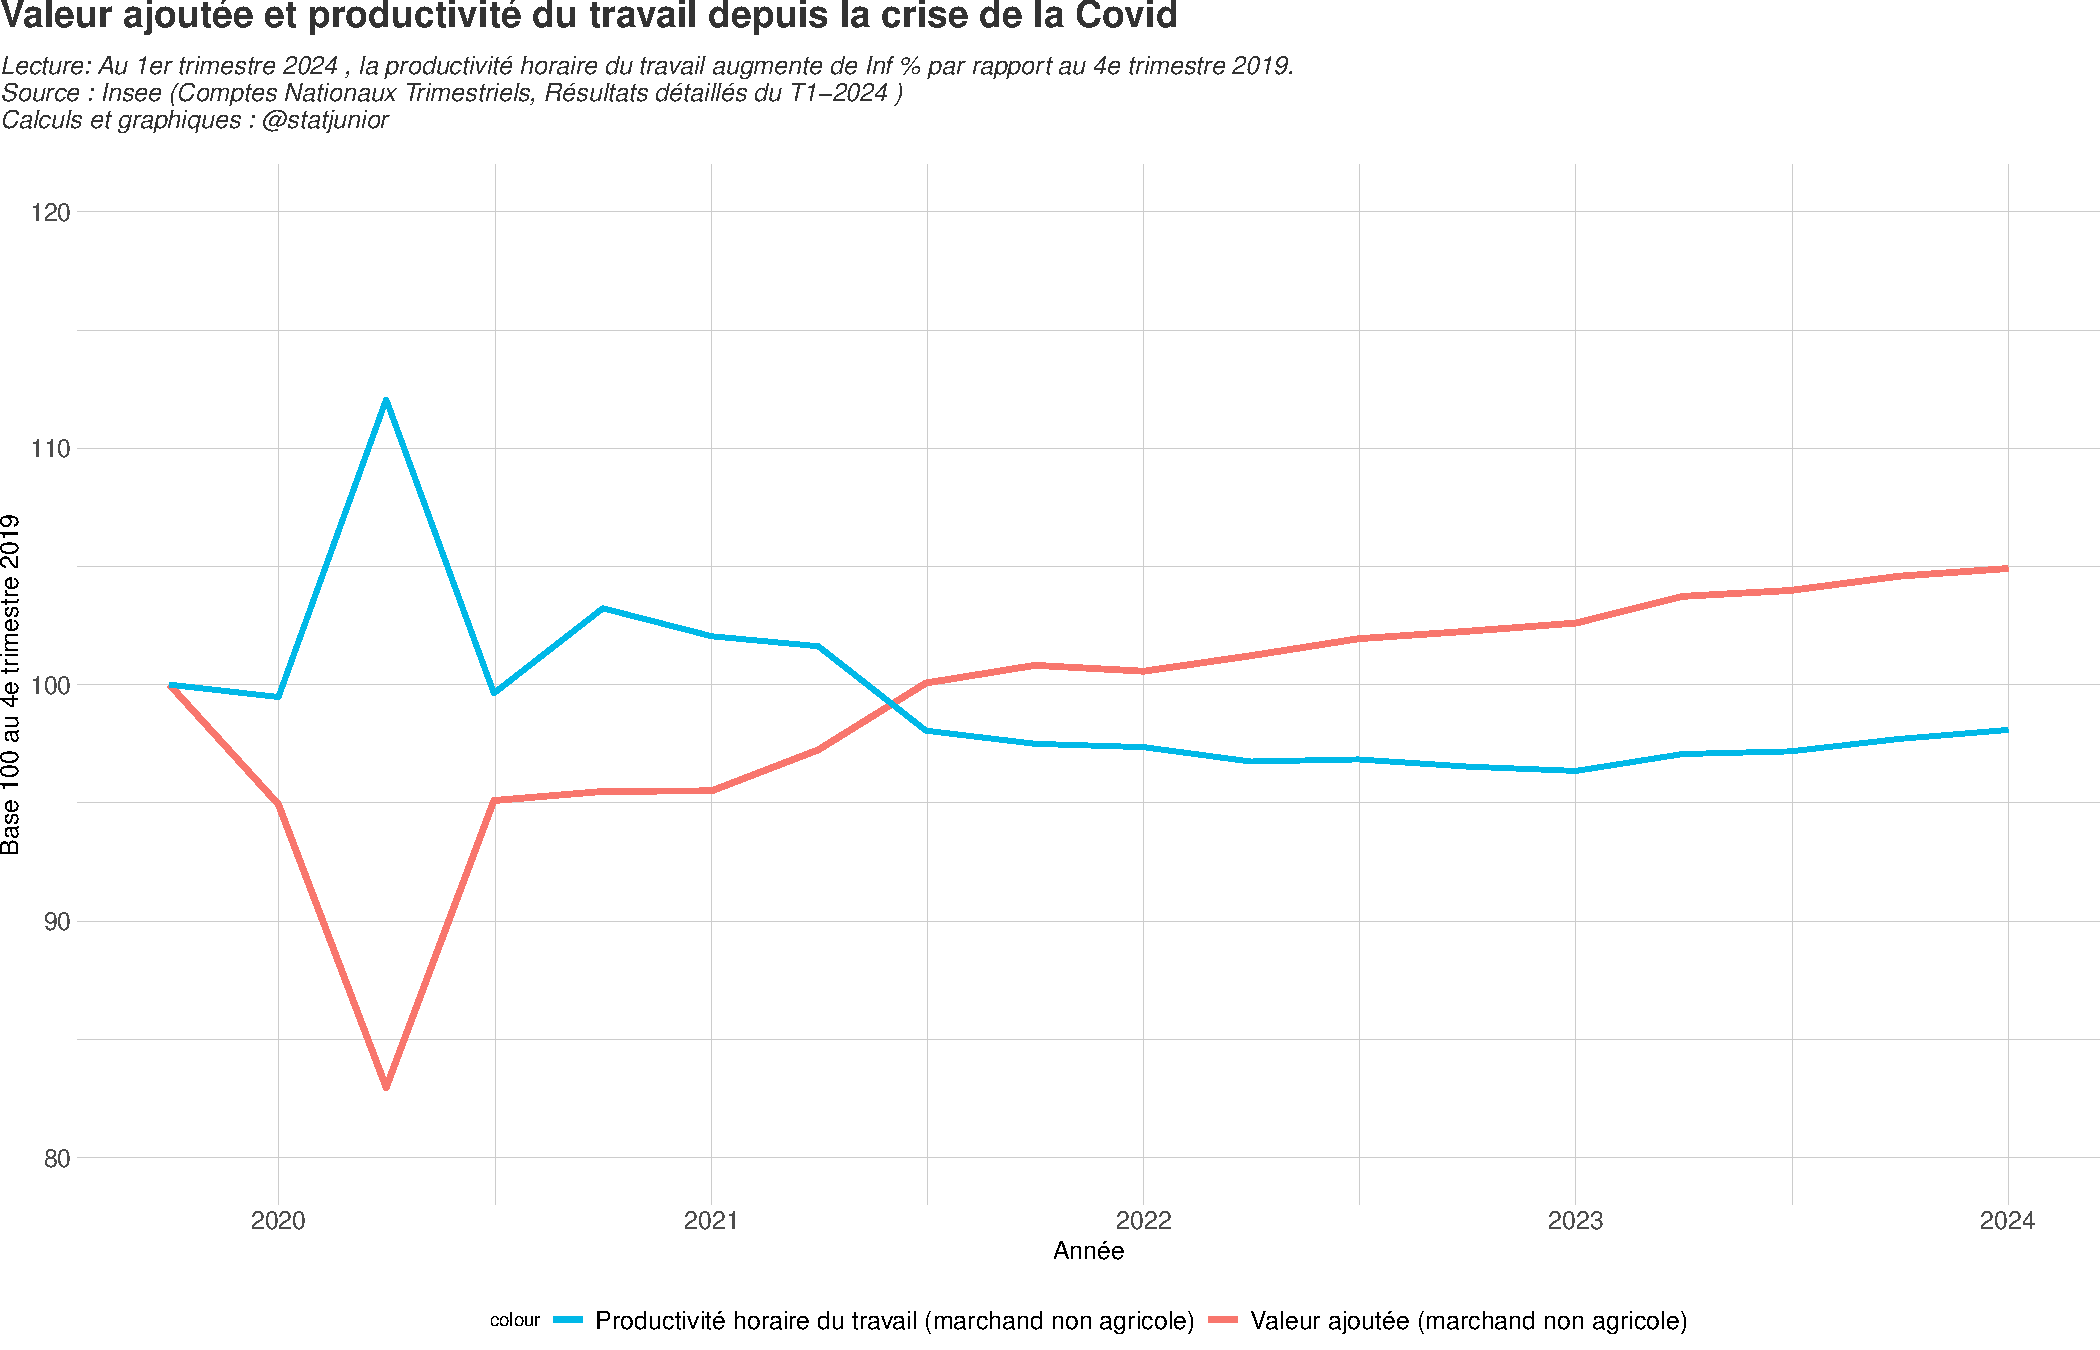
\includegraphics{rapport_pdf_compte_branche_files/figure-latex/unnamed-chunk-21-1.pdf}

\hypertarget{duxe9composition-du-taux-de-marge-par-contribution-productivituxe9-masse-salariale-cotisations-sociales-termes-de-luxe9change-autres-facteurs}{%
\subsection{Décomposition du taux de marge par contribution
(productivité, masse salariale, cotisations sociales, termes de
l'échange, autres
facteurs)}\label{duxe9composition-du-taux-de-marge-par-contribution-productivituxe9-masse-salariale-cotisations-sociales-termes-de-luxe9change-autres-facteurs}}

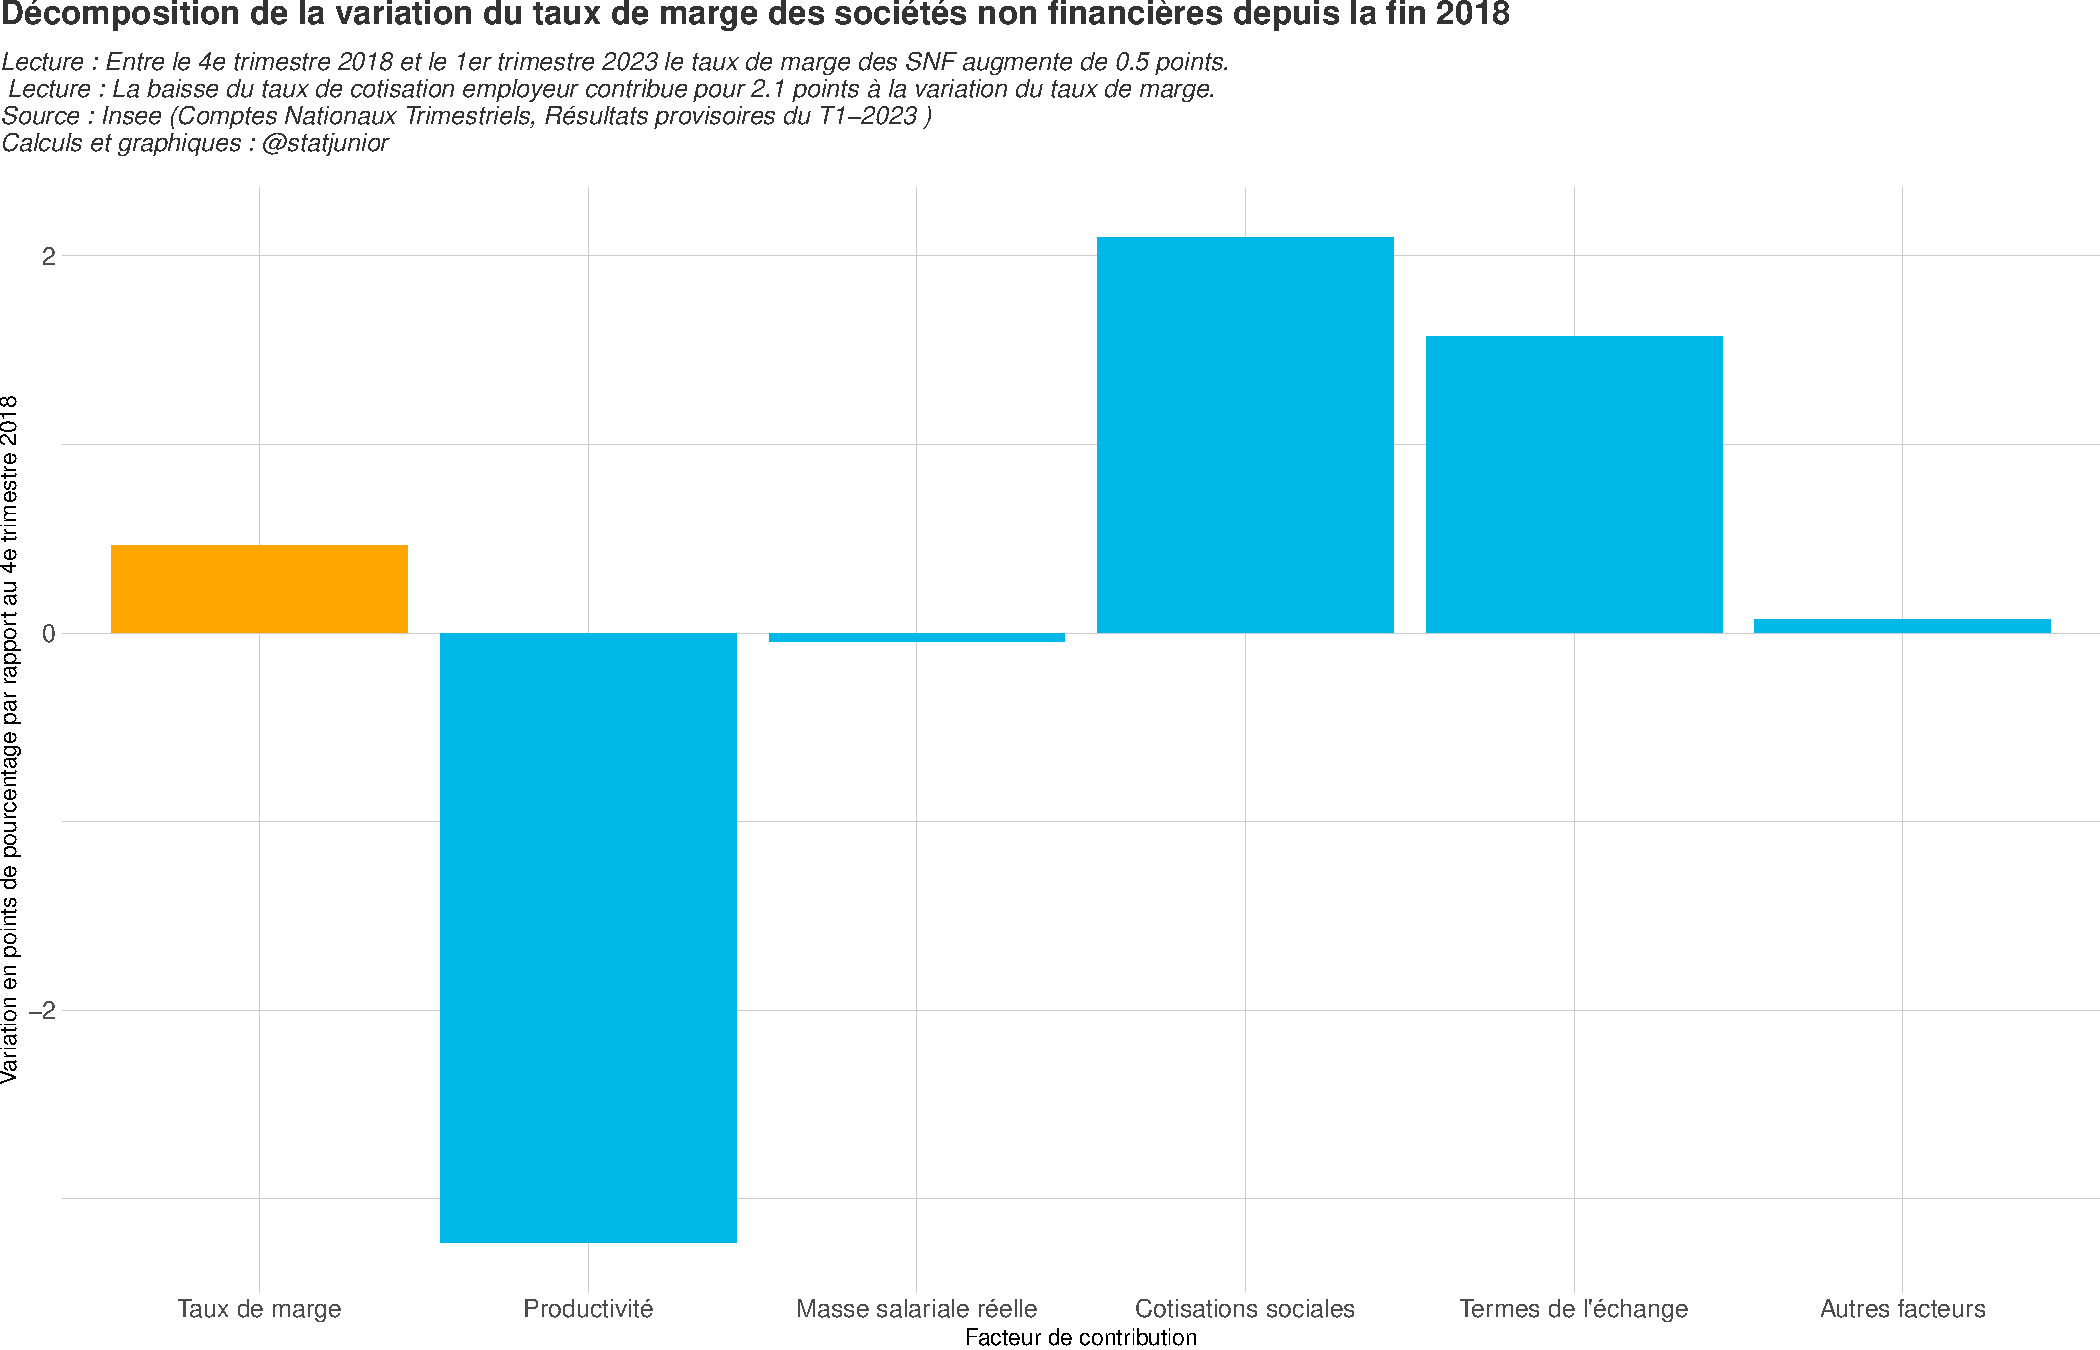
\includegraphics{rapport_pdf_compte_branche_files/figure-latex/unnamed-chunk-22-1.pdf}

\hypertarget{evolution-du-taux-de-marge-par-secteur-par-rapport-uxe0-lannuxe9e-2018}{%
\subsection{Evolution du taux de marge par secteur par rapport à l'année
2018}\label{evolution-du-taux-de-marge-par-secteur-par-rapport-uxe0-lannuxe9e-2018}}

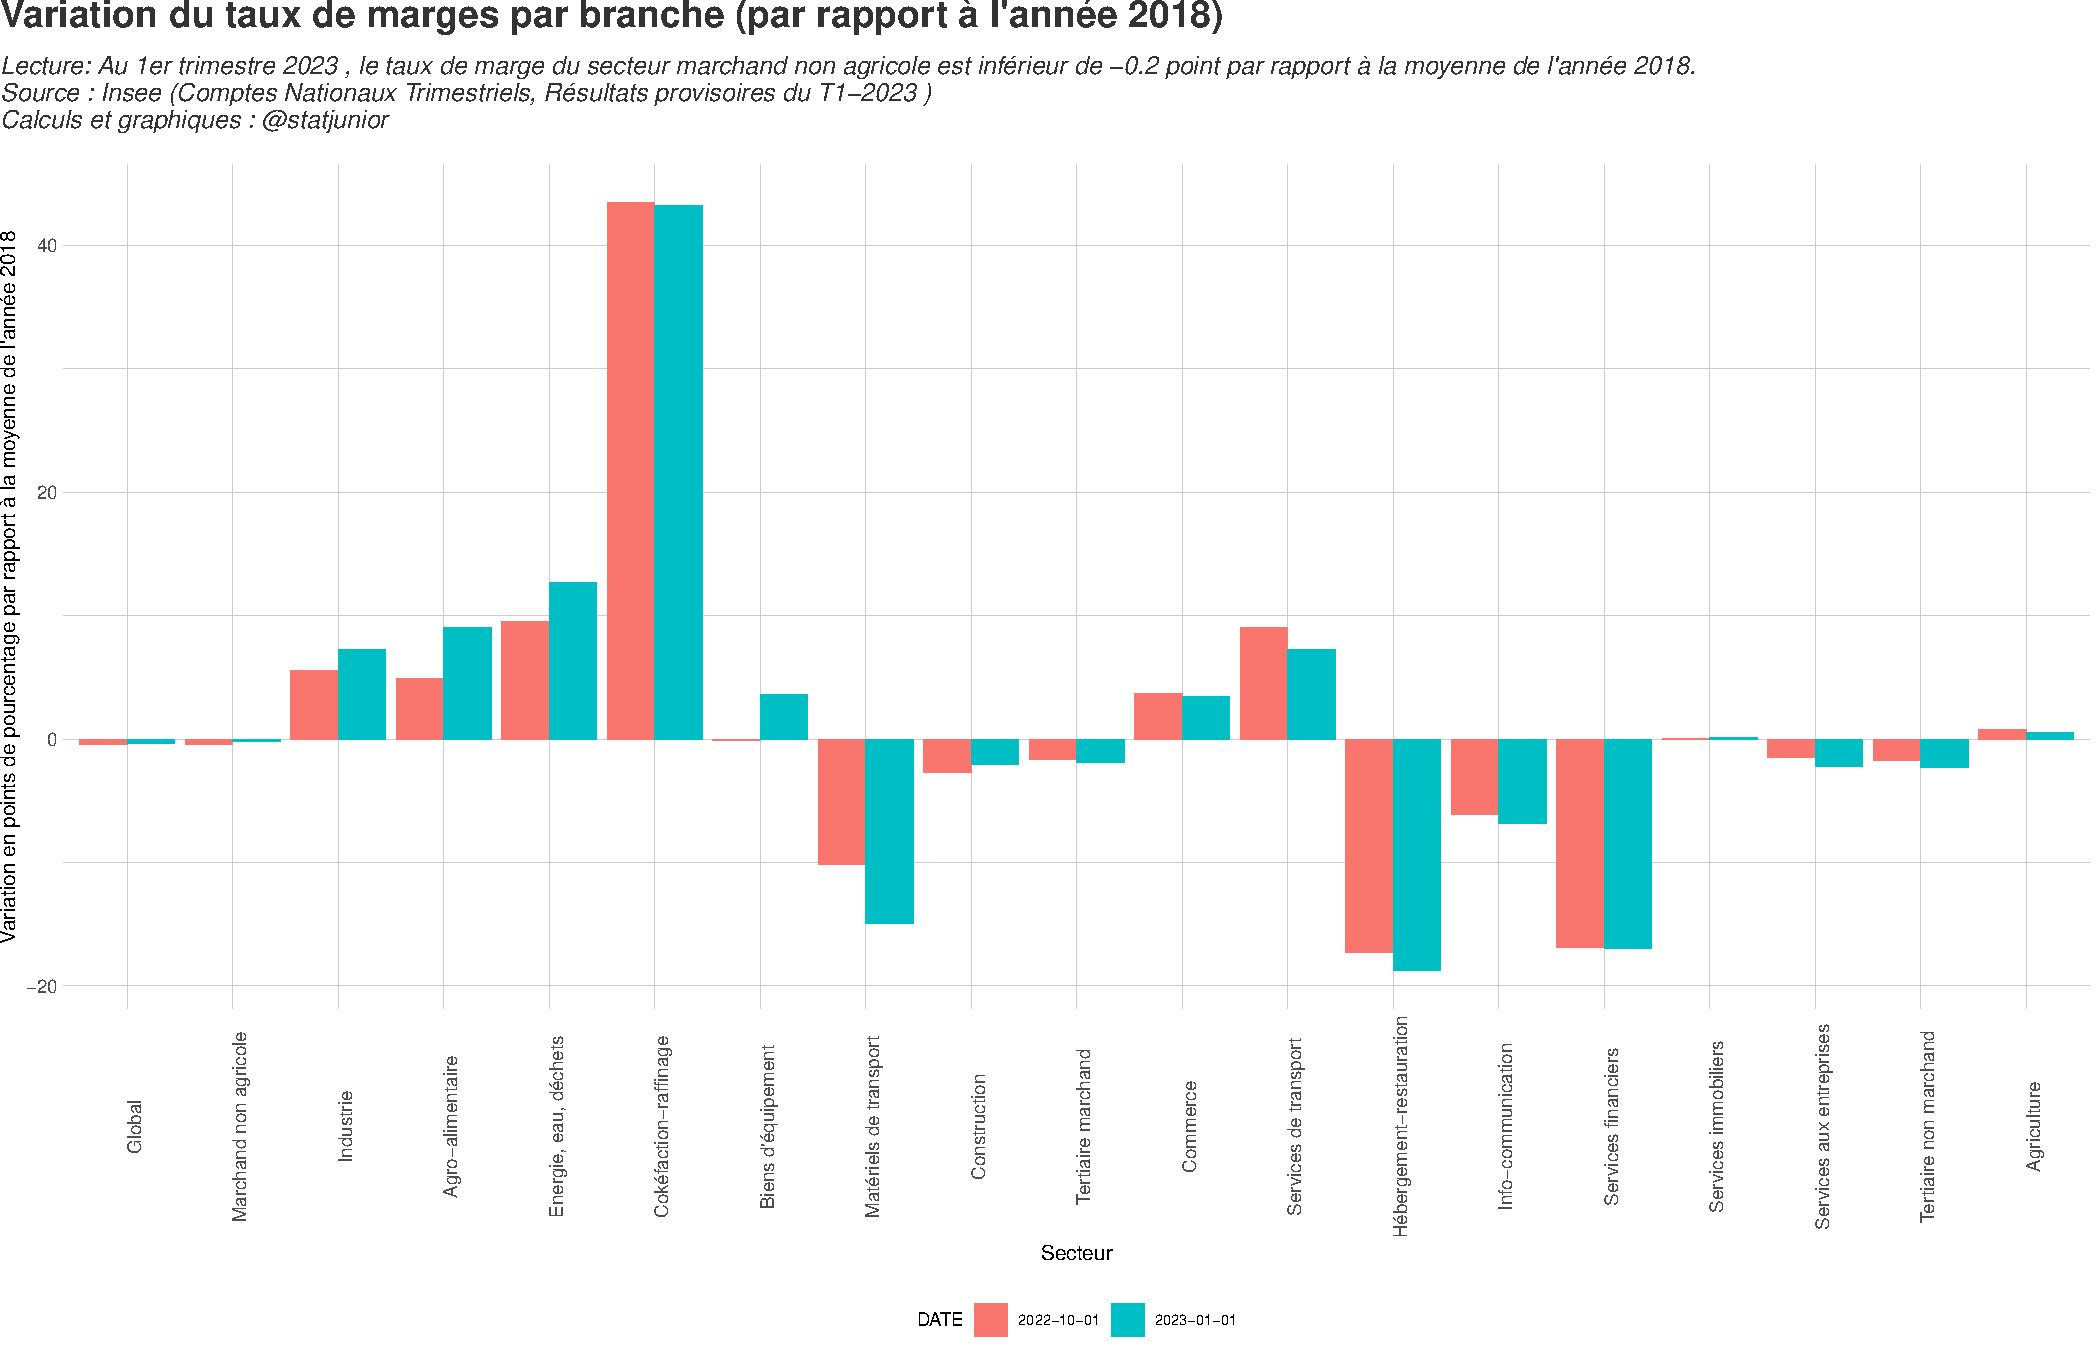
\includegraphics{rapport_pdf_compte_branche_files/figure-latex/unnamed-chunk-23-1.pdf}

\newpage

\hypertarget{profits-exceptionnels-liuxe9s-aux-tensions-inflationnistes-depuis-2021}{%
\section{Profits exceptionnels liés aux tensions inflationnistes depuis
2021}\label{profits-exceptionnels-liuxe9s-aux-tensions-inflationnistes-depuis-2021}}

\hypertarget{taux-de-marge-des-secteurs-uxe9nerguxe9tiques-et-des-services-de-transport}{%
\subsection{Taux de marge des secteurs énergétiques et des services de
transport}\label{taux-de-marge-des-secteurs-uxe9nerguxe9tiques-et-des-services-de-transport}}

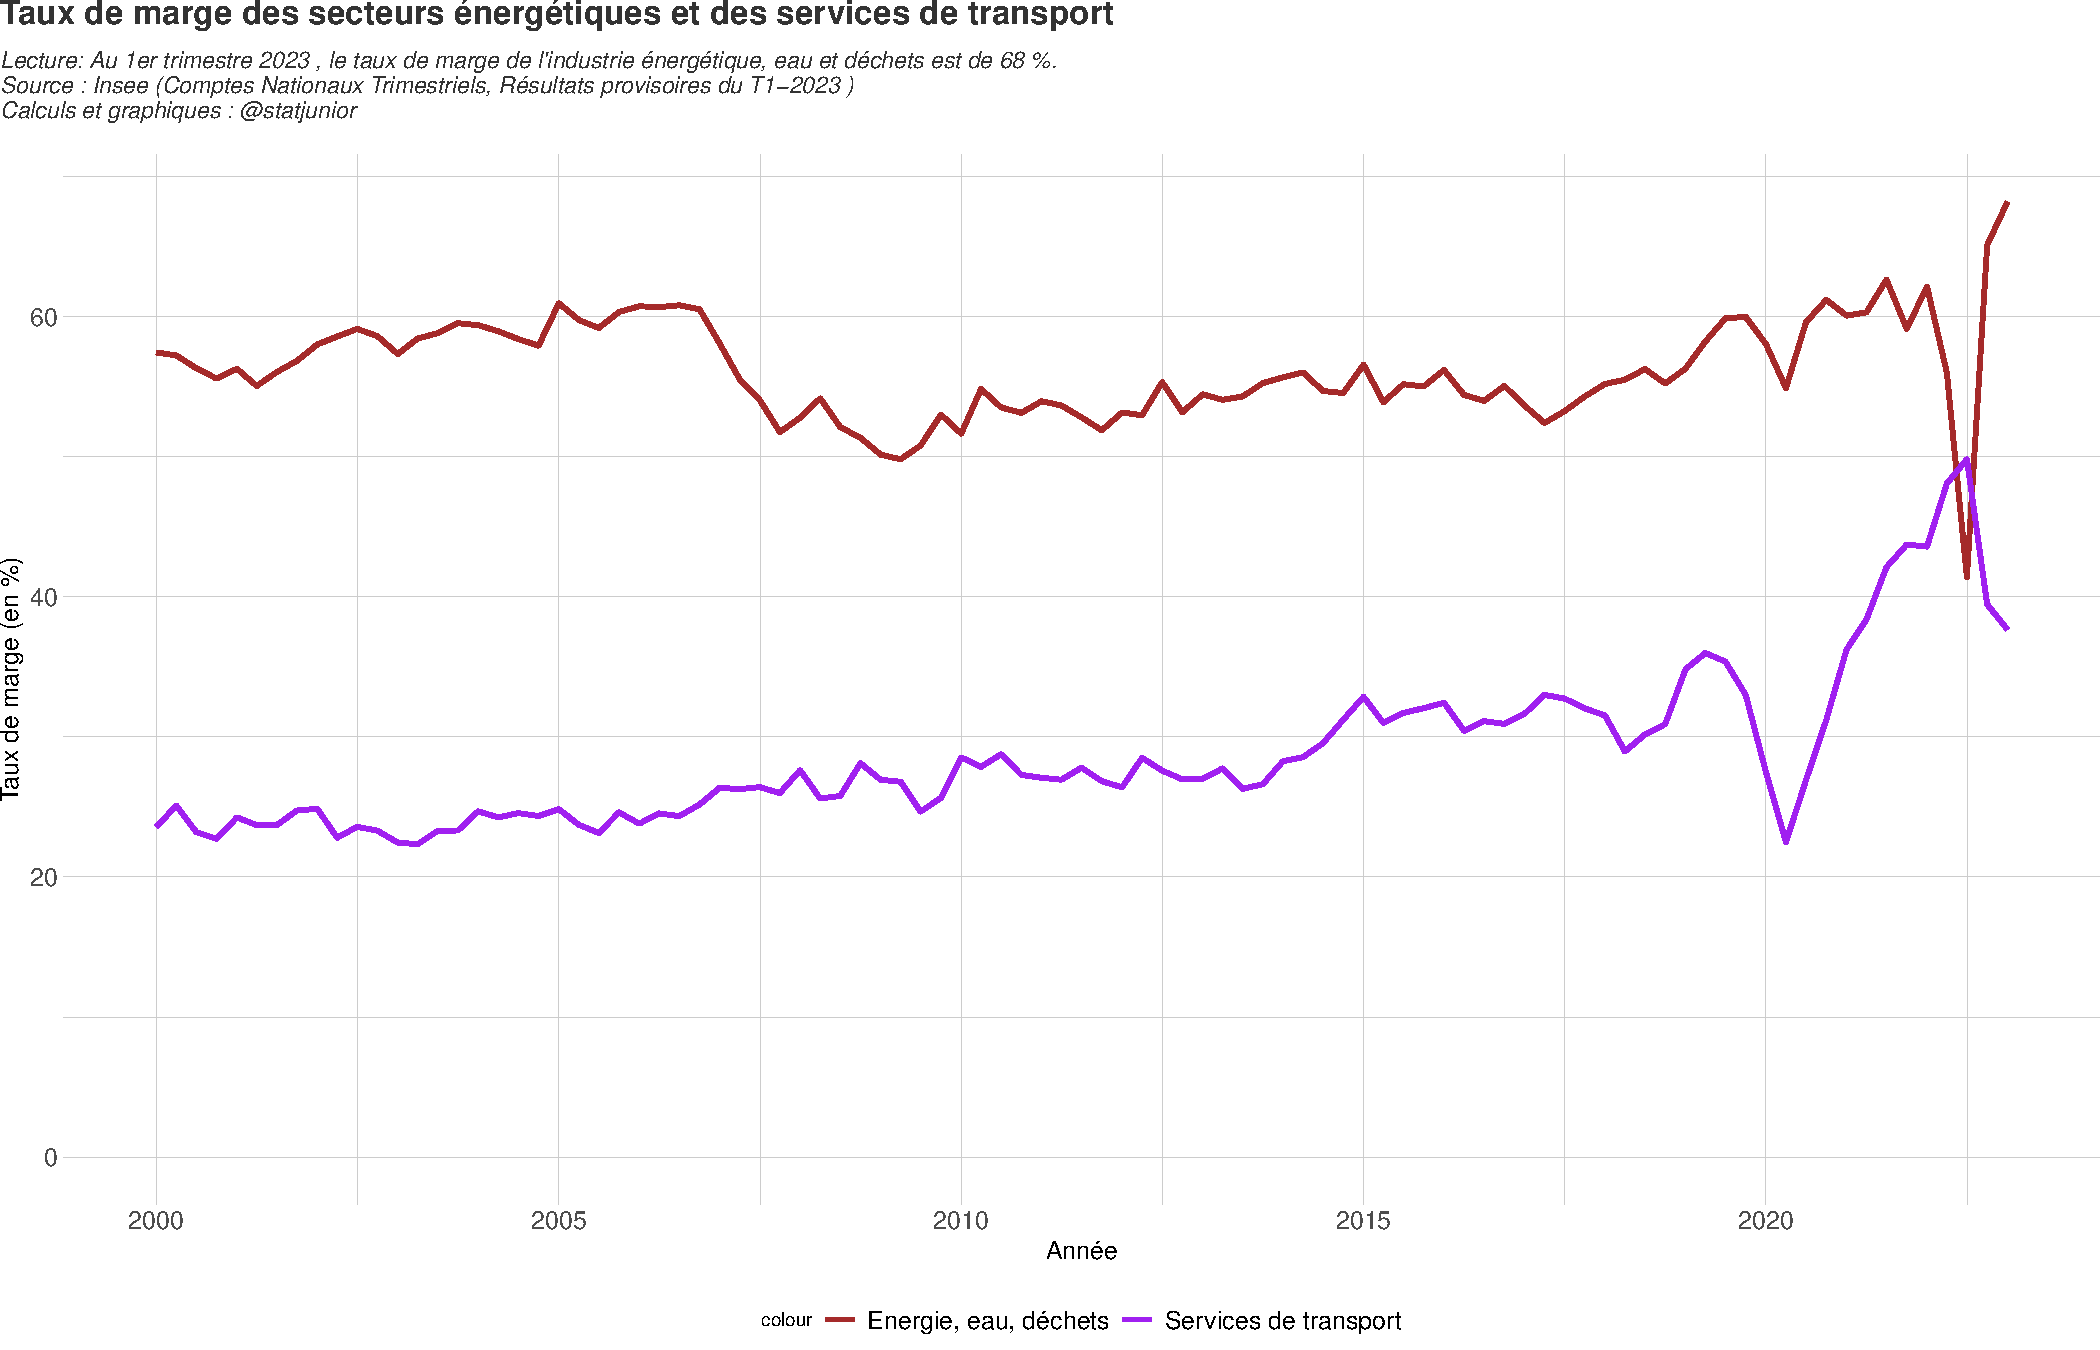
\includegraphics{rapport_pdf_compte_branche_files/figure-latex/unnamed-chunk-25-1.pdf}

\hypertarget{taux-de-marge-de-lindustrie-cockuxe9faction---raffinage}{%
\subsection{Taux de marge de l'industrie cockéfaction -
raffinage}\label{taux-de-marge-de-lindustrie-cockuxe9faction---raffinage}}

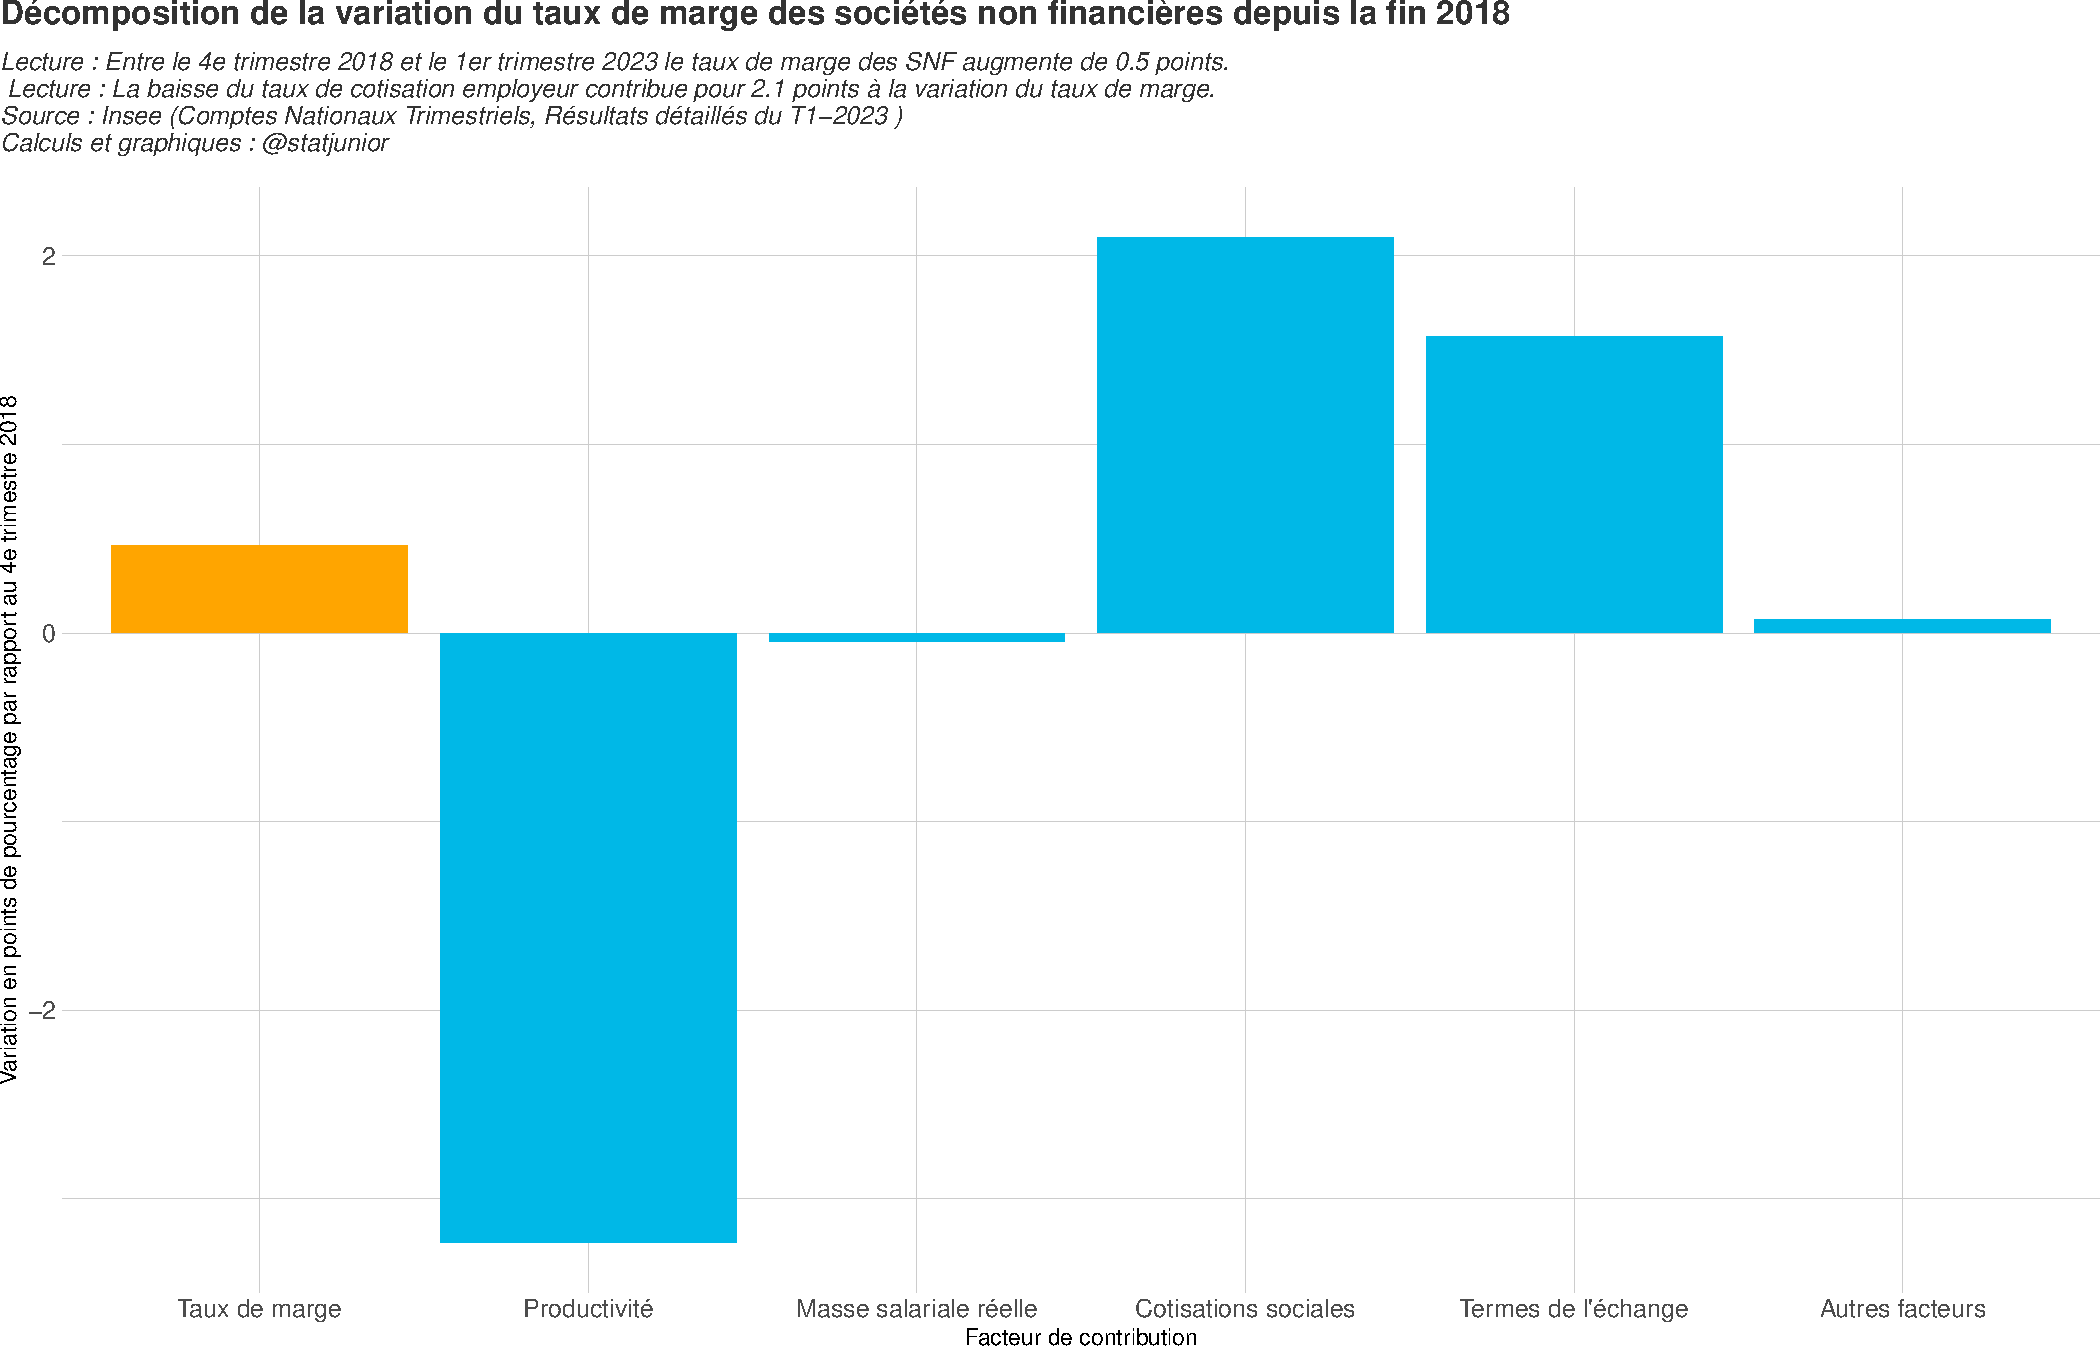
\includegraphics{rapport_pdf_compte_branche_files/figure-latex/unnamed-chunk-27-1.pdf}

\hypertarget{taux-de-marge-de-lindustrie-agro-alimentaire}{%
\subsection{Taux de marge de l'industrie
agro-alimentaire}\label{taux-de-marge-de-lindustrie-agro-alimentaire}}

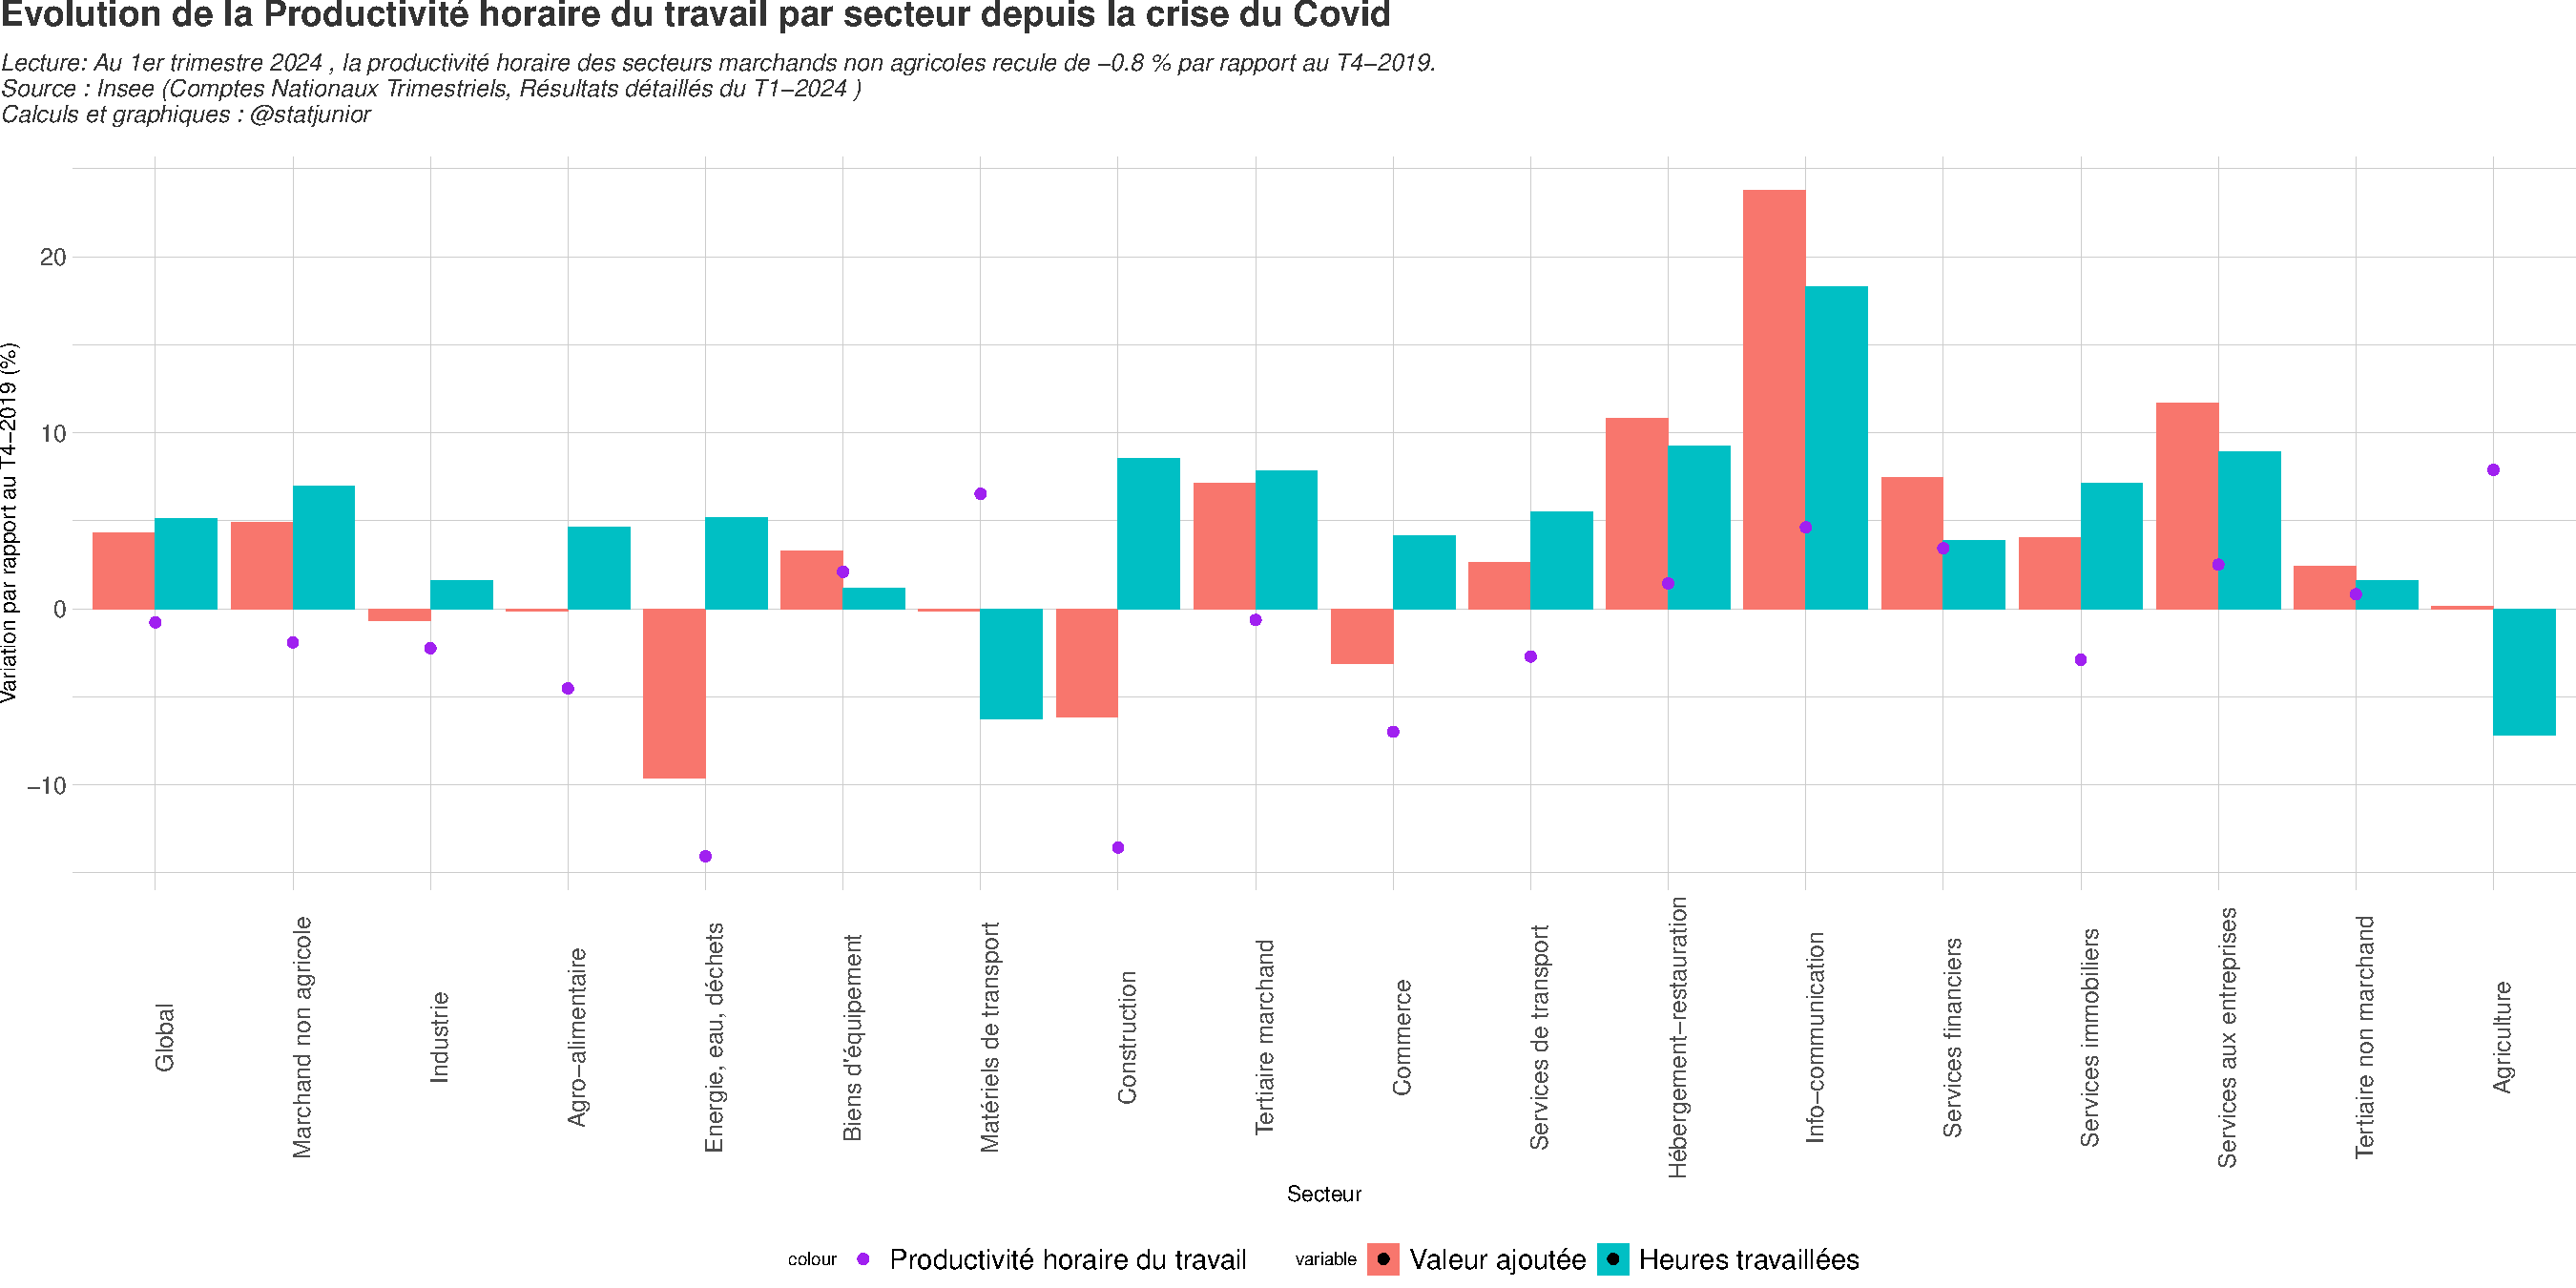
\includegraphics{rapport_pdf_compte_branche_files/figure-latex/unnamed-chunk-28-1.pdf}

\hypertarget{part-des-profits-exceptionnels-des-secteurs-uxe9nerguxe9tiques-dans-lensemble-de-la-valeur-ajoutuxe9e-franuxe7aise}{%
\subsection{Part des profits exceptionnels des secteurs énergétiques
dans l'ensemble de la valeur ajoutée
française}\label{part-des-profits-exceptionnels-des-secteurs-uxe9nerguxe9tiques-dans-lensemble-de-la-valeur-ajoutuxe9e-franuxe7aise}}

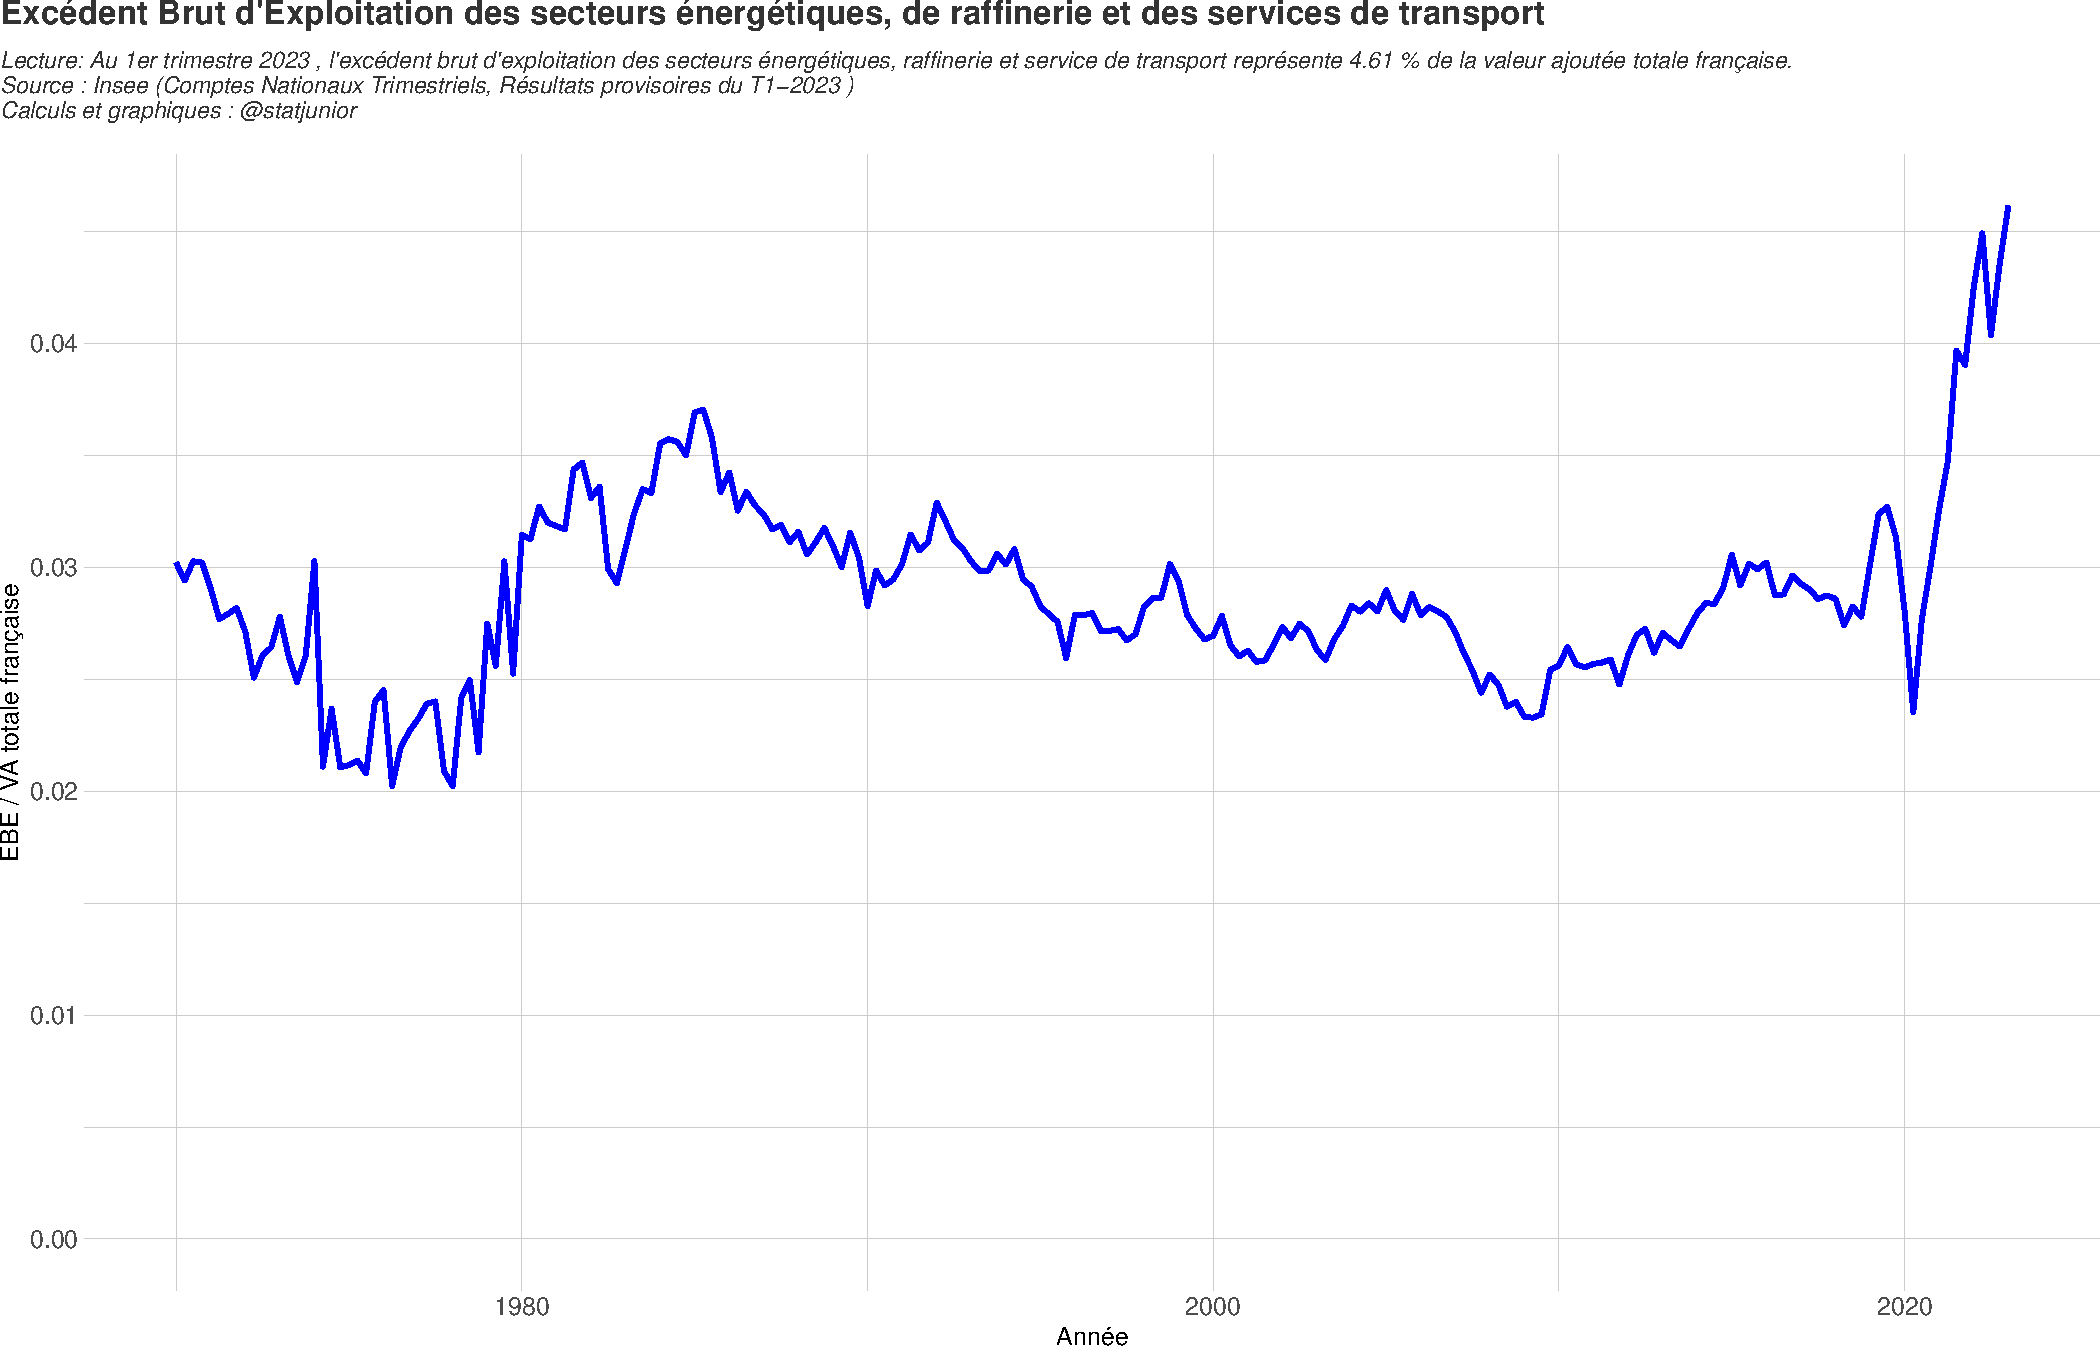
\includegraphics{rapport_pdf_compte_branche_files/figure-latex/unnamed-chunk-29-1.pdf}

\hypertarget{part-des-profits-exceptionnels-des-secteurs-uxe9nerguxe9tiques-et-de-lindustrie-agro-alimentaire-dans-luxe9conomie-franuxe7aise}{%
\subsection{Part des profits exceptionnels des secteurs énergétiques et
de l'industrie agro-alimentaire dans l'économie
française}\label{part-des-profits-exceptionnels-des-secteurs-uxe9nerguxe9tiques-et-de-lindustrie-agro-alimentaire-dans-luxe9conomie-franuxe7aise}}

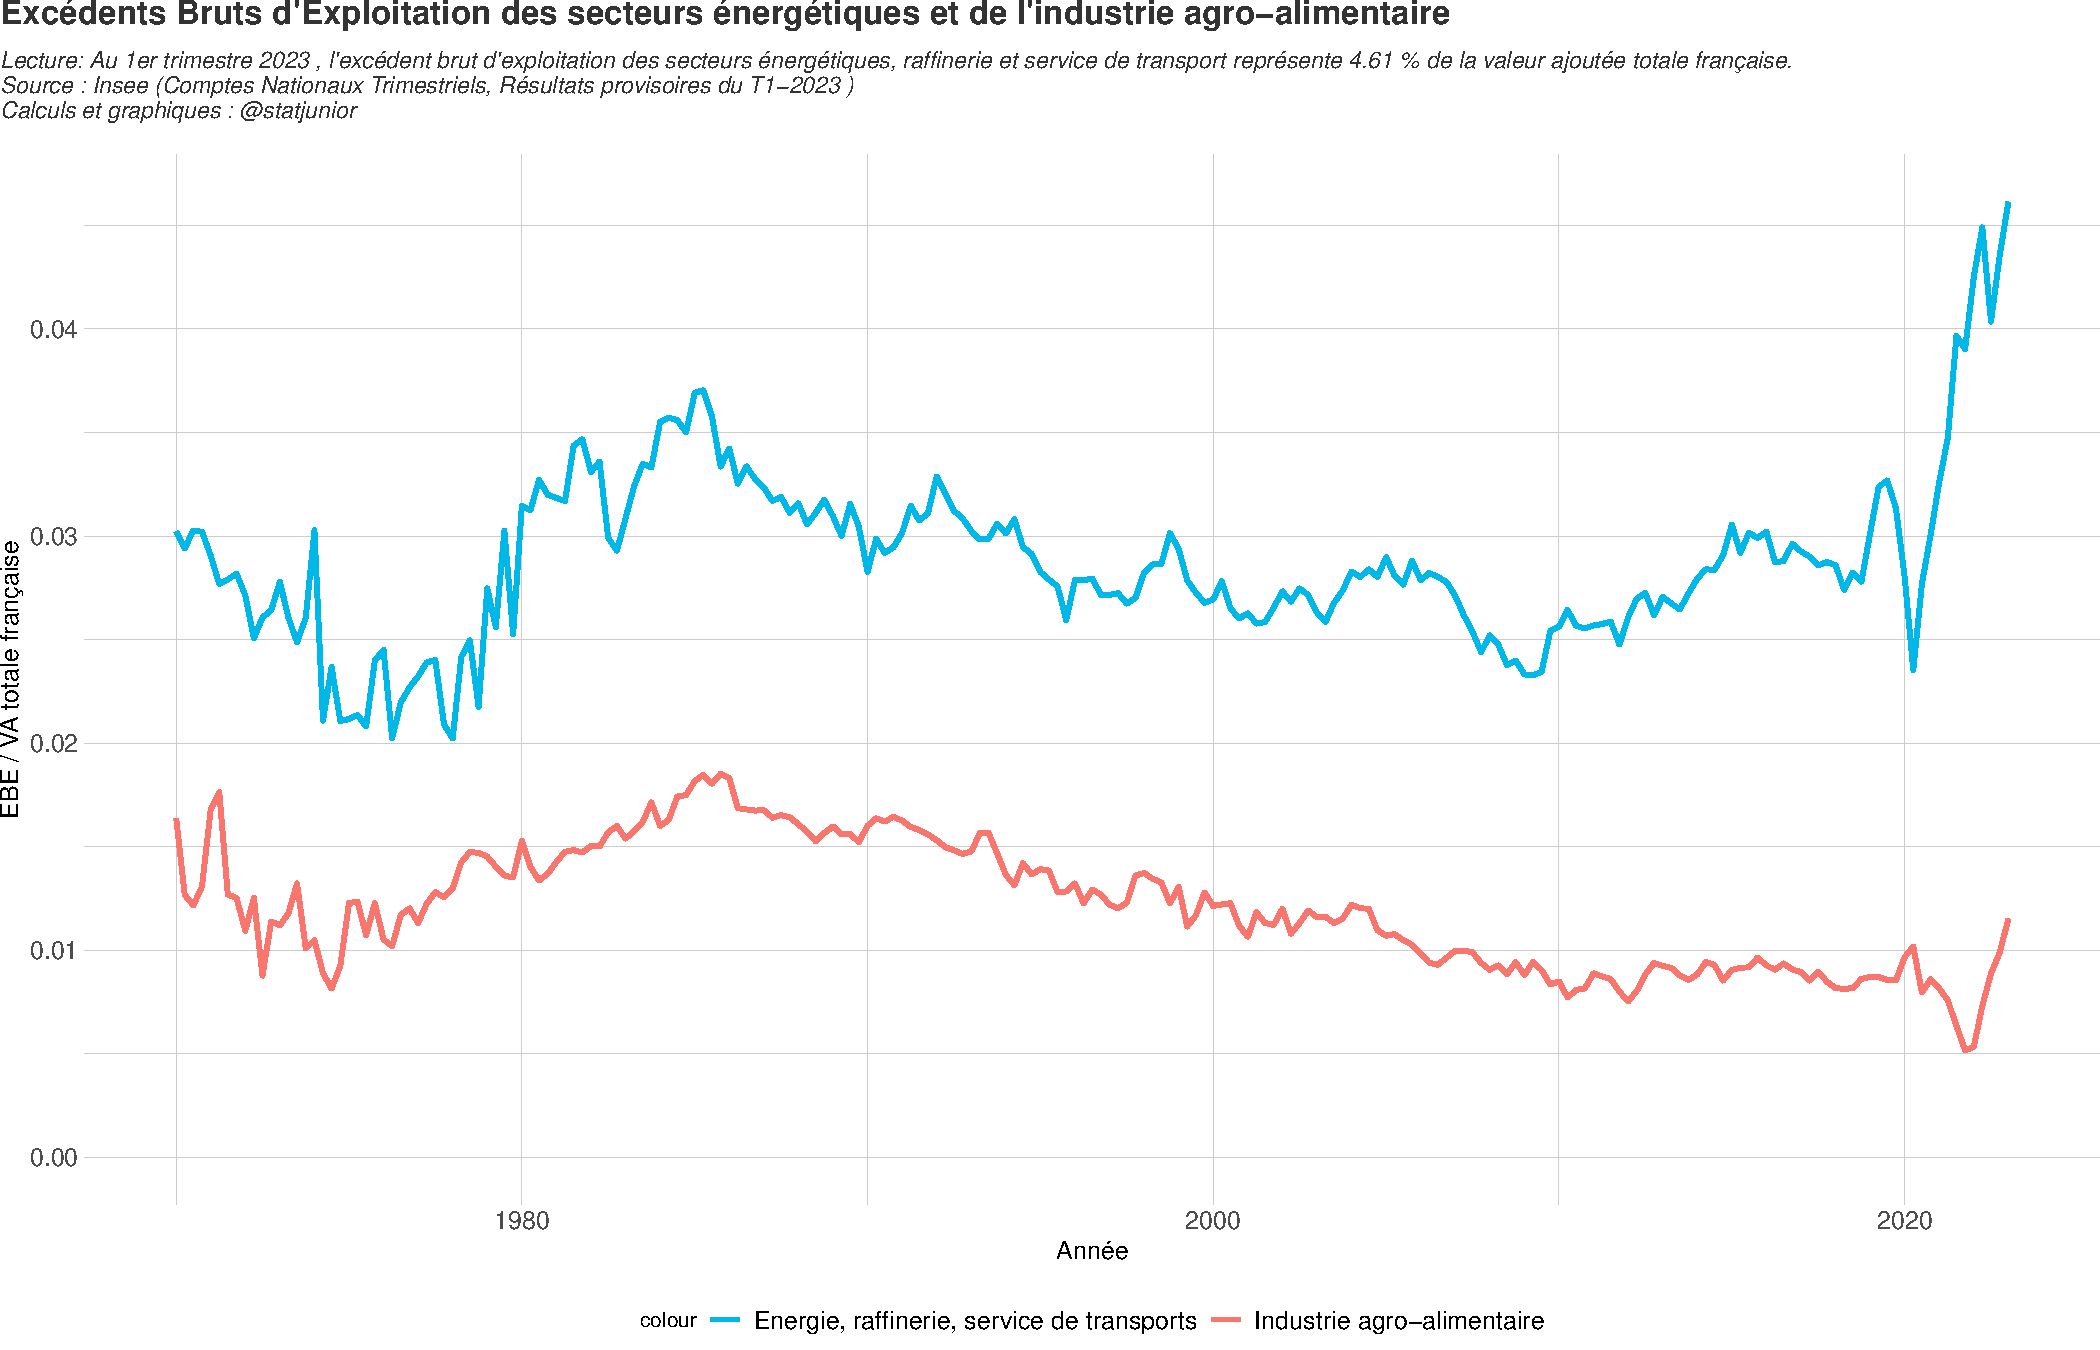
\includegraphics{rapport_pdf_compte_branche_files/figure-latex/unnamed-chunk-30-1.pdf}

\end{document}
